\documentclass{jknotes}
\usepackage{joshkirklin}

\begin{document}

\institution{Cambridge Part III Maths}
\title{Black Holes}
\lecturer{Harvey Reall}
\notetaker{Josh Kirklin}
\date{Lent 2016}

\maketitle
\suggestionsspiel
In this course we take \(G=c=1\) and \(\Lambda=0\).
\tableofcontents

\section{Spherical stars}
\lecture{15/01/16}
Consider a gas of cold fermions. This gas will resist compression due to \emph{degeneracy pressure} resulting from the Pauli principle. For example, in a white dwarf star, gravity is balanced by electron degeneracy pressure. Using Newtonian gravity, we can find an upper limit on the mass of a stable white dwarf, known as the \emph{Chandrasekhar limit}:
\begin{equation}
    M_{\text{WD}} \lesssim 1.4M_{\astrosun}
\end{equation}

In a neutron star, gravity is balanced by neutron degeneracy pressure. Neutron stars are tiny; a neutron star with the mass of the sun has a radius of approximately \SI{10}{\kilo\meter} (for comparison, the sun has a radius of \(R_{\astrosun}\approx\SI{7e5}{\kilo\meter}\). At the surface of a neutron star, the gravitational potential \(|\phi|\approx0.1\). Recall that in order to be able to apply Newtonian gravity, we must have \(|\phi|\ll1\). \(0.1
\not\ll1\), so it is important to consider general relativity when reasoning about neutron stars.

In this section we will establish that \(M \lesssim 3M_{\astrosun}\) for \emph{any} cold star.

\subsection{Spherical symmetry and time independence}

Consider the round metric on \(S^2\):
\begin{equation}
    \dd{\Omega}^2 = \dd{\theta}^2+\sin^2\theta\dd{\phi}^2
\end{equation}
Equipped with this metric, if we exclude reflections, \(S^2\) has \(SO(3)\) as its isometry group. This motivates the following:
\begin{defn}
    A spacetime is \emph{spherically symmetric} if its isometry group has an \(SO(3)\) subgroup whose orbits are 2-spheres.
\end{defn}
\begin{defn}
    The \emph{area-radius function} \(r:\mathcal{M}\rightarrow\RR\) is defined by:
    \begin{equation}
        A(p) = 4\pi r(p)^2,\quad r(p)\ge 0
    \end{equation}
where \(A(p)\) is the area of the \(SO(3)\) orbit through \(p\).
\end{defn}
A consequence of this is that the induced metric on the \(SO(3)\) orbit through \(p\) is \(r(p)^2\dd{\Omega}^2\).

\begin{defn}
    \((\mathcal{M},g)\) is \emph{stationary} if it permits a timelike Killing vector field (KVF).
\end{defn}

\begin{wrapfigure}{L}{0.3\textwidth}
    \centering
    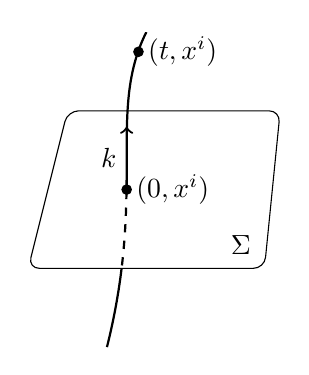
\begin{tikzpicture}
        \draw[rounded corners] (0,0) -- (0.5,2) -- (3.2,2) -- (3,0) -- cycle;
        \def\killingone{\draw[thick] (1,-1) .. controls (1.5,1) and (1,2) .. (1.5,3)}
        \begin{scope}
            \clip (0,0) rectangle (3,-1);
            \killingone;
        \end{scope}
        \begin{scope}[dashed]
            \clip (0,1) rectangle (3,0);
            \killingone;
        \end{scope}
        \begin{scope}
            \clip (0,1) rectangle (3,3);
            \killingone;
        \end{scope}
        \draw[fill] (1.25,1) circle (0.06) node[right] {\((0,x^i)\)};
        \draw[->,thick] (1.25,1) -- (1.25,1.8) node[midway,left] {\(k\)};
        \draw[fill] (1.4,2.75) circle (0.06) node[right] {\((t,x^i)\)};
        \node at (2.7,0.3) {\(\Sigma\)};
    \end{tikzpicture}
\end{wrapfigure}

Suppose we have a stationary spacetime with timelike Killing vector \(k\). Let \(\Sigma\) be a spacelike 3 dimensional hypersurface, and let \(x^i\), \(i=1,2,3\) be coordinates on \(\Sigma\).

We define coordinates for the manifold in the following way: from each point \((x^1,x^2,x^3)\) extend an integral curve of \(k\); the point \((t,x^i)\) is a parameter distance \(t\) along this curve.

In the chart \((t,x^i)\), we can write:
\begin{equation}
    k=\pdv{t}
\end{equation}
Then, using the defining property of Killing vectors, we have that the metric is independent of \(t\). Thus, we can write:
\begin{equation}
    \dd{s}^2 = g_{00}(x^k)\dd{t}^2 + 2g_{0i}(x^k)\dd{t}\dd{x^i} + g_{ij}(x^j)\dd{x^i}\dd{x^j}
\end{equation}
and we have \(g_{00}<0\) since \(k\) is timelike.

Suppose we have a surface \(\Sigma\) given by \(f(x)=0\), where \(f:\mathcal{M}\rightarrow\RR\), \(\dd{f}|_\Sigma\ne0\). Then \(\dd{f}\) is normal to \(\Sigma\). Suppose \(n\) is another 1-form that is normal to \(\Sigma\). Then we can write \(n=g\dd{f}+fn'\), where \(g\) is a function and \(n'\) is some 1-form. We have:
\begin{equation}
    \dd{n} = \dd{g}\wedge\dd{f}+g\underbrace{\dd[2]{f}}_{=0} + \dd{f}\wedge n' + f\dd{n'}
\end{equation}
\begin{equation}
    \implies \dd{n}|_\Sigma = (\dd{g}-n')\wedge\dd{f} \implies n\wedge \dd{n}|_\Sigma = 0
\end{equation}
In fact, the converse is true:
\begin{theorem}[Frobenius]
    If \(n\) is a 1-form such that \(n\wedge \dd{n}=0\), then there exist functions \(f,g\) such that \(n=g\dd{f}\), so that \(n\) is normal to surfaces of constant \(f\).
\end{theorem}
If \(n\) is a 1-form of this type, we say it is \emph{hypersurface-orthogonal}.

\begin{defn}
    \((\mathcal{M},g)\) is \emph{static} if it contains a hypersurface-orthogonal timelike KVF.
\end{defn}

Suppose we are in a static spacetime, and define coordinates \(t,x^i\) as before. \(\Sigma\) is a surface of constant \(t\), so we have \(k \propto dt\), \(k_\mu \propto (1,0,0,0)\). Also note that \(k_\mu = g_{\mu\nu}k^\nu = g_{\mu\nu}(\pdv{t})^\nu = (g_{00},g_{10},g_{20},g_{30})\). Hence we can deduce that \(g_{i0}=0\), and can write the metric as:
\begin{equation}
    \dd{s}^2 = g_{00}(x^k) \dd{t}^2 + g_{ij}(x^k)\dd{x^i}\dd{x^j}
\end{equation}
where as before \(g_{00}<0\). In this metric we have a discrete isometry \((t,x^i) \rightarrow (-t,x^i)\). A static metric must be time-independent \emph{and} invariant under time reversal. A simple case of a stationary but not static metric is that associated with a rotating star. If we reverse time the star spins in the other direction.

\subsection{Static, spherically symmetric spacetimes}
If we have a spacetime that is both stationary and spherically symmetric, then the isometry group must contain:
\begin{equation}
    \underbrace{\RR}_{\substack{\text{time}\\\text{translation}}} \times \underbrace{SO(3)}_{S^2 \text{ orbits}}
\end{equation}
It can be shown that with this condition the spacetime must also be static.

Let \(\Sigma_t \perp k^a\) be a foliation of the spacetime, and use coordinates \((r,\theta,\phi)\) on each surface, where \(\theta,\phi\) are the usual spherical coordinates and \(r\) is the area-radius function as defined earlier. Then we must have:
\begin{equation}
    \dd{s}^2|_{\Sigma_t} = e^{2\Psi(r)}\dd{r}^2 + r^2\dd{\Omega}
\end{equation}
for some function \(\Psi(r)\). Note that we have no \(\dd{r}\dd{\theta}\) or \(\dd{r}\dd{\phi}\) terms because they would violate spherical symmetry. If we define \(t\) as above we can then write the entire metric as:
\begin{equation}
    \dd{s}^2 = -e^{2\Phi(r)}\dd{t}^2 + e^{2\Psi(r)}\dd{r}^2 + r^2\dd{\Omega}
\end{equation}
for some other function \(\Phi(r)\).

\subsection{The TOV equations}
Consider now the matter inside a stationary and spherically symmetric star. We will model the star as a perfect fluid, which means we have the following energy-momentum tensor:
\begin{equation}
    T_{ab} = (\rho+P)u_au_b + \rho g_{ab}
\end{equation}
where \(\rho\) is the energy density, \(P\) is the pressure, and \(u_a\) is the 4-velocity of the fluid. Since the star is stationary, we can assume the fluid is at rest, so \(u^a = e^{-\Phi}\left( \pdv{t} \right)^a\) (since \(u\) is a unit vector pointing in the \(t\) direction). Also, since we have spherical symmetry we can assume that \(\rho\) and \(P\) are functions of \(r\) only.

\lecture{18/01/16}
Make the following definition:
\begin{equation}
    e^{2\Psi(r)} = \left( 1 - \frac{2m(r)}{r} \right)^{-1}
\end{equation}
Note that since \(e^{2\Psi(r)}>0\), we have \(m(r) < \frac{r}{2}\). Using the Einstein field equations \(G = 8\pi T\) it is now possible to derive the \emph{Tolman-Oppenheimer-Volkoff equations}:

\begin{equation}
    \dv{m}{r} = 4\pi r^2\rho
    \tag{TOV1}
    \label{TOV1}
\end{equation}
\begin{equation}
    \dv{\Phi}{r} = \frac{m+4\pi r^3P}{r(r-2m)}
    \tag{TOV2}
    \label{TOV2}
\end{equation}
\begin{equation}
    \dv{P}{r} = - (P+\rho) \frac{m+4\pi r^3P}{r(r-2m)}
    \tag{TOV3}
    \label{TOV3}
\end{equation}
We now have three equations, but four unknowns (\(m\),\(\Phi\),\(\rho\) and \(P\)). In order to solve this system, we will need a fourth equation, and the one most commonly chosen is an equation of state relating \(P\) and \(\rho\). In a cold star, we can assume that the temperature \(T(\rho,P)=0\) and we can solve this to get \(P\) explicitly in terms of \(\rho\):
\begin{equation}
    P = P(\rho)
\end{equation}
This is called a \emph{barotropic} equation of state.

We will assume that \(\rho,P>0\). We will also assume that \(\dv{P}{\rho}>0\); this is a stability condition\footnote{Consider \(\dv{P}{\rho}<0\). Then if \(\rho\) increases by a small amount in a region \(R\), \(P\) decreases in \(R\), but then this causes more fluid to flow into \(R\), increasing \(\rho\) further.}. 

Let the radius of the star be \(R\).
\begin{description}
    \item[Outside the star] (\(r>R\)) we can assume \(\rho = P = 0\). \eqref{TOV1} then gives that \(m(r) = M\) a constant. \eqref{TOV2} further provides that \(\Phi = \frac{1}{2}\log\left( 1-\frac{2M}{r} \right) + \Phi_0\), where \(\Phi_0\) is another constant. Note that since \(g_tt = -e^{2\Phi} \rightarrow e^{-2\Phi_0}\) as \(r\rightarrow\infty\), we can eliminate \(\Phi_0\) by making a change of coordinates \(t\rightarrow e^{\Phi_0}t\), so w.l.o.g. we assume that \(\Phi_0 = 0\).
        Hence we have the \emph{Schwarzschild metric}:
        \begin{equation}
            \dd{s}^2 = - \left( 1 - \frac{2M}{r} \right)\dd{t}^2 + \left( 1 - \frac{2M}{r} \right)^{-1}\dd{r}^2 + r^2\dd{\Omega}^2
        \end{equation}
        By taking \(r\) to be large and comparing with Newtonian gravity, we can deduce that \(M\) is in fact the mass of the star.
        Note that this metric has a problem. It is singular at the so-called \emph{Schwarzschild radius} \(r=2M\). Thus a static, spherically symmetric star must have \(R>2M\) (in a normal star, \(R\gg2M\)).
    \item[Inside the star] (\(r<R\)), we now have matter to deal with. Integrating \eqref{TOV1}, we have:
        \begin{equation}
            m(r) = 4\pi\int_0^r\rho(r')r'^2\dd{r'}+m_*
        \end{equation}
        where \(m_*\) is a constant. Consider a constant \(t\) hypersurface. The induced line element on this hypersurface is \(\dd{s}^2 = e^{2\Psi}\dd{r}^2 + r^2\dd{\Omega}^2\). The proper radius (i.e. distance to \(r=0\)) of a point is given by \(\int_0^re^{\Psi(r')}\dd{r'}\). In order for our spacetime to be a manifold, we require that it is locally flat at \(r = 0\), and this requires that the proper radius tends to the area-radius as \(r\rightarrow 0\). Note that
        \(\int_0^re^{\Psi(r')}\dd{r'} \sim e^{\Psi(0)}r\) as \(r\rightarrow 0\), so we require that \(e^{\Psi(0)} = 1\), or equivalently \(m(0) = 0\). From this we deduce that \(m_*=0\). 

        If we match this expression on the boundary of the star to the Schwarzschild solution for the exterior, we see that \(m(R)=M\), or:
        \begin{equation}
            M = 4\pi\int_0^R\rho(r)r^2\dd{r}
            \tag{\(*\)}
            \label{match}
        \end{equation}
        The volume form on a constant \(t\) hypersurface is \(e^\Psi r^2\sin\theta \dd{r}\wedge\dd{\theta}\wedge\dd{\phi}\), and so the energy of the matter in the star for \(t\) constant is:
        \begin{equation}
            E = 4\pi\int_0^R\rho e^\Psi r^2\dd{r}
        \end{equation}
        Note that since \(m\) is increasing, so is \(e^\Psi\) and hence \(e^\Psi\ge1\) for all \(0 \le r \le R\). Thus we have \(E > M\). The reason for this is that we have a gravitational binding energy \(E-M\).

        If we evaluate \(\frac{m(r)}{r}<\frac{1}{2}\) at \(r=R\) we see that \(\frac{M}{R} < \frac{1}{2}\). In fact it is possible to improve this: \eqref{TOV3} \(\implies\dv{P}{r}\le0\implies\dv{\rho}{r}\le0\), and from this we can deduce:
        \begin{equation}
            \frac{m(r)}{r} < \frac{2}{9}\left( 1 - 6\pi r^2P(r) + \left[ 1 + 6\pi r^2P(r) \right]^{\frac{1}{2}} \right)
            \tag{\(\dagger\)}
            \label{buchdahl}
        \end{equation}
        Setting \(r = R\) and noting \(P(R) = 0\), we obtain the so-called \emph{Buchdahl inequality}: \(\frac{M}{R}<\frac{4}{9}\).

        In general, we must solve this system of equations numerically. \eqref{TOV1} and \eqref{TOV3} are a pair of coupled first order ODEs for \(m(r)\) and \(\rho(r)\), from which we can obtain a unique solution given \(m(0)=0\) and specifying \(\rho(0) = \rho_c\), the central density. From \eqref{TOV3} we have that \(P\) is decreasing in \(r\), so \(R(\rho_c)\) is determined by fixing \(P(R) = 0\). Then, using \eqref{match} we can obtain \(M(\rho_c)\). Finally, using
        \eqref{TOV2} and the boundary condition that \(\Phi(R) = \frac{1}{2}\log\left( 1 - \frac{2M}{R} \right)\) we can deduce \(\Phi(r)\). 

        To summarise, given an equation of state, static, spherically symmetric, cold stars are a 1-parameter family labelled by \(\rho_c\).
\end{description}

\subsection{Maximum mass}
We wish to find a limit on the maximum mass of a star.
\begin{figure}[H]
    \centering
    \begin{tikzpicture}[scale=1.5]
        \draw[domain=0:3,smooth,variable=\x] plot({\x},{\x*(3.2-\x)/2});
        \draw[thick,->] (0,0) -- (3.5,0) node[right] {\(\rho_c\)};
        \draw[thick,->] (0,0) -- (0,1.6) node[above] {\(M\)};
        \draw[dashed] (0,1.28) node[left] {\(M_{\text{max}}\)} -- (3.5,1.28);
    \end{tikzpicture}
\end{figure}
In general, \(M_{\text{max}}\) depends on the equation of state, but here we run into a problem: we do not know the equation of state in certain conditions, namely \(\rho>\rho_0\), where \(\rho_0\) is typically on the order of the density of an atomic nucleus.

\begin{wrapfigure}{l}{0.5\linewidth}
    \centering
    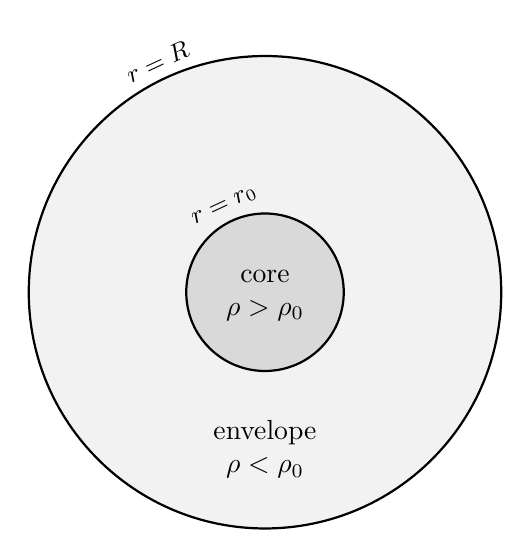
\begin{tikzpicture}
        \fill[gray!10] (0,0) circle (3);
        \fill[gray!30] (0,0) circle (1);
        \draw[thick] (0,0) circle (3);
        \draw[thick] (0,0) circle (1);

        \node at (0,0) {
            \begin{tabular}{c}
                core \\
                \(\rho>\rho_0\)
            \end{tabular}
            };
        \node at (0,-2) {
            \begin{tabular}{c}
                envelope \\
                \(\rho<\rho_0\)
            \end{tabular}
            };
        
        \node[above,rotate=25,shift={(0,1)}] at (0,0) {\small\(r=r_0\)};
        \node[above,rotate=25,shift={(0,3)}] at (0,0) {\small\(r=R\)};
    \end{tikzpicture}
\end{wrapfigure}
Remarkarbly, it is still possible to find an upper bound on the mass of a star. We do this by splitting the star into two regions: an \emph{envelope}, in which we know the equation of state (so \(\rho<\rho_0\)), and a \emph{core}, in which we do not (\(\rho>\rho_0\)). Since \(\dv{\rho}{r}<0\), the envelope does in fact envelope the core.

Let \(m_0 = m(r_0)\); we call this the \emph{core mass}. Since the minimum density in the core is \(\rho_0\), we have \(m_0\ge\frac{4}{3}\pi r_0^3\rho_0\). Additionally, we can apply \eqref{buchdahl} at \(r=r_0\) to obtain:
\begin{equation}
    \frac{m_0}{r_0} < \frac{2}{9}\left( 1 - 6\pi r_0^2P_0 + \left[ 1 + 6\pi r_0^2P_0 \right]^{\frac{1}{2}} \right)
\end{equation}
where \(P_0=P(\rho_0)\). This is a decreasing function of \(P_0\), so \(\frac{m_0}{r_0}<\frac{4}{9}\).

Lets plot these two constraints:
\begin{figure}[H]
    \centering
    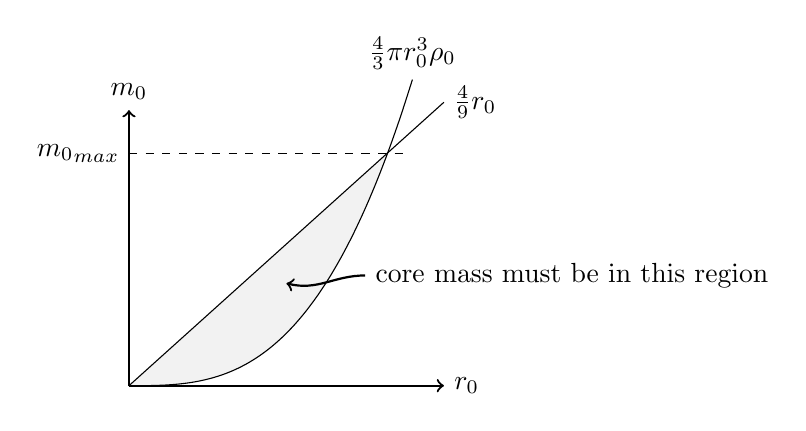
\begin{tikzpicture}
        \begin{scope}
            \clip (0,0) -- (4,0) -- (4,3.6) -- cycle;
            \fill[gray!10,domain=0:3.6,smooth,variable=\x] plot({\x},{\x^3/12});
        \end{scope}
        \draw[domain=0:3.6,smooth,variable=\x] plot({\x},{\x^3/12}) node[above] {\(\frac{4}{3}\pi r_0^3\rho_0\)};
        \draw[domain=0:4,smooth,variable=\x] plot({\x},{\x*0.9}) node[right] {\(\frac{4}{9}r_0\)};
        \draw[thick,->] (0,0) -- (4,0) node[right] {\(r_0\)};
        \draw[thick,->] (0,0) -- (0,3.5) node[above] {\(m_0\)};
        \draw[dashed] (0,2.95) node[left] {\({m_0}_{\text{max}}\)} -- (3.5,2.95);

        \draw[thick,<-] (2,1.3) .. controls (2.4,1.2) and (2.6,1.4) .. (3,1.4) node[right] {core mass must be in this region};
    \end{tikzpicture}
\end{figure}
We see that we have an upper bound on the core mass. Solving for this upper bound, we find:
\begin{equation}
    m_0 < \sqrt{\frac{16}{23\pi\rho_0}}
\end{equation}
If \(\rho_0\approx\) nuclear density, then we have \(m_0 \lesssim 5M_{\astrosun}\).

Now we can extend our solution to the envelope. \(m_0\) and \(r_0\) together uniquely determine the envelope, as we can solve \eqref{TOV1} and \eqref{TOV3} starting at \(r=r_0\) and using the known equation of state for \(\rho<\rho_0\). From this we obtain \(M\) as a function of \(m_0\) and \(r_0\), and so can find the maximal value of \(M\) when \(m_0,r_0\) take values in the region in the graph above.

Numerically, we can find that \(M\) is maximised when \(m_0\) is maximised, and that the maximum mass is \(M\approx m_0\approx5M_{\astrosun}\).

In fact, it is possible to improve this limit by imposing that the speed of sound is physical, i.e.\ less than the speed of light: \(\sqrt{\dv{P}{\rho}}\le1\). Using this gives \(M \lesssim 3M_{\astrosun}\).

\section{The Schwarzschild solution}
\lecture{20/01/16}
We showed earlier that the only static, spherically symmetric solution of the vacuum EFEs is the Schwarzschild solution:
\begin{equation}
    \dd{s}^2 = - \left( 1-\frac{2M}{r} \right)\dd{t}^2 + \left( 1-\frac{2M}{r} \right)^{-1}\dd{r}^2 + r^2\dd{\Omega}^2
\end{equation}
\(t,r,\theta,\phi\) are known as \emph{Schwarzschild coordinates}. We will assume \(M>0\).

In fact:
\begin{theorem}[Birkhoff]
    Any spherically symmetric solution of the vacuum Einstein equations is isometric to the Schwarzschild solution.
\end{theorem}
So in particular, spherical symmetry and a vacuum implies a static spacetime (for \(r>2M\)).

\subsection{Gravitational redshift}
Consider two fixed observers \(A,B\) in a Schwarzschild spacetime. \(A\) sends two photons to \(B\), seperated by a time \(\Delta t\).

\begin{wrapfigure}{l}{0.4\linewidth}
    \centering
    \begin{tikzpicture}
        \draw[thick,->] (-1.5,-1.5) -- (-0.8,-1.5) node[right] {\(r\)};
        \draw[thick,->] (-1.5,-1.5) -- (-1.5,-0.8) node[above] {\(t\)};
        \draw[thick] (0,0) -- (0,-4) node[below] {\(A\)};
        \draw[thick] (3,0) -- (3,-4) node[below] {\(B\)};
        \fill (0,-3) circle (0.07);
        \fill (3,-1.5) circle (0.07);
        \fill (0,-2.5) circle (0.07);
        \fill (3,-1) circle (0.07);
        \draw[photon] (0,-3) -- (3,-1.5);
        \draw[photon] (0,-2.5) -- (3,-1);
        \draw[thick,<->] (-0.2,-3) -- (-0.2,-2.5) node[midway,left] {\(\Delta t\)};
        \draw[thick,<->] (3.2,-1.5) -- (3.2,-1) node[midway,right] {\(\Delta t\)};
    \end{tikzpicture}
\end{wrapfigure}
Because \(\pdv{t}\) is an isometry of the spacetime, the second photon's path is the same as that of the first, but translated by \(\Delta t\). Consider the 4-velocity of a fixed observer. We have:
\begin{equation}
    -1 = u^\mu u_\mu = g_{tt}\left(\dv{t}{\tau}\right)^2 = - \left( 1-\frac{2M}{r} \right)\left(\dv{t}{\tau}\right)^2
\end{equation}
Hence we have \(\dd{\tau} = \sqrt{1 - \frac{2M}{r}}\dd{t}\). Therefore the proper time intervals between the photons at \(A\) and \(B\) are:
\begin{equation}
    \Delta\tau_A = \sqrt{1-\frac{2M}{r_A}}\Delta t
    ,\quad
    \Delta\tau_B = \sqrt{1-\frac{2M}{r_B}}\Delta t
\end{equation}
So we have:
\begin{equation}
    \frac{\Delta \tau_B}{\Delta \tau_A} = \frac{\sqrt{1 - \frac{2M}{r_B}}}{\sqrt{1-\frac{2M}{r_A}}}
\end{equation}
If we suppose that the photons were sent at two subsequent wavecrests, then \(\Delta \tau\) is the period of the waves, equal to \(\lambda\), the wavelength (since \(c=1\)). We define the redshift \(z\) by:
\begin{equation}
    1 + z = \frac{\lambda_B}{\lambda_A} = \frac{\sqrt{1 - \frac{2M}{r_B}}}{\sqrt{1-\frac{2M}{r_A}}}
\end{equation}
For \(r_B > r_A\), we have \(z>0\), so light is redshifted as it climbs out of the gravitational field. For \(r_B\gg 2M\):
\begin{equation}
    1 + z = \sqrt{\frac{1}{1 - \frac{2M}{r_A}}}
\end{equation}
Note that this \(\rightarrow \infty\) as \(r_A\rightarrow2M\).

For a star, we have the Buchdahl inequality, \(R>\frac{9}{4}M\), so plugging this into the above, we find that the maximum redshift from the surface of a spherical star is \(z=2\).

\subsection{Geodesics}
Suppose \(x^\mu(\tau)\) is an affinely parametrised geodesic, and let its 4-velocity be \(u^\mu = \dv{x^\mu}{\tau}\). We have Killing fields \(k=\pdv{t}\) and \(m=\pdv{\phi}\), so along geodesics we have two conserved quantities:
\begin{equation}
    E=-k\vdot u = \left( 1-\frac{2M}{r} \right)\dv{t}{\tau}
    \qq{and}
    h = m\vdot u = r^2\sin^2\theta\dv{\phi}{\tau}
\end{equation}
If our geodesic is timelike and we choose \(\tau\) to be proper time, we can identify \(E\) as the energy per unit mass and \(h\) as the angular momentum per unit mass associated with the geodesic.

In the null case, we can define the \emph{impact parameter} \(b = \left|\frac{h}{E}\right|\), and identify this as the limit of the distance between the geodesic and the star perpendicular to the geodesic as \(r\rightarrow 0\).
\begin{figure}[H]
    \centering
    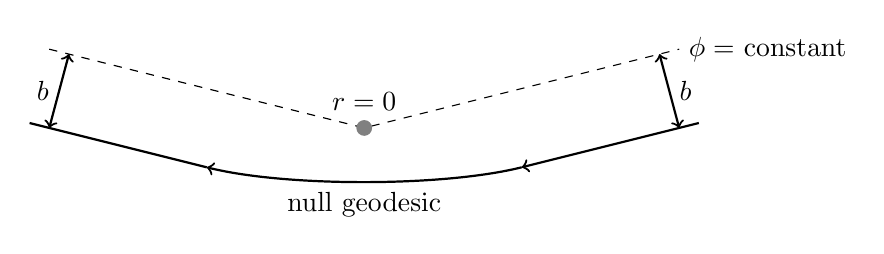
\begin{tikzpicture}
        \draw[dashed] (-4,1) -- (0,0) -- (4,1) node[right] {\(\phi = \) constant};
        \fill[gray] (0,0) circle (0.1);
        \node[above] at (0,0.1) {\(r=0\)};
        \draw[thick,->] (4.25,0.0625) -- (2,-0.5); 
        \draw[thick,->] (2,-0.5) .. controls (1,-0.75) and (-1,-0.75) .. (-2,-0.5) node[below, midway] {null geodesic};
        \draw[thick] (-2,-0.5) -- (-4.25,0.0625);
        \draw[thick,<->] (3.75,0.9375) -- (4,0) node[midway,right] {\(b\)};
        \draw[thick,<->] (-3.75,0.9375) -- (-4,0) node[midway,left] {\(b\)};
    \end{tikzpicture}
\end{figure}

equationéeieieieieiee

Exercises:
\begin{enumerate}
    \item Derive the Euler-Lagrange equation for \(\theta(\tau)\). Show that one can choose coordinates such that \(\theta(\tau) = \frac{\pi}{2}\), so that motion is contained in the equatorial plane.
    \item Rearrange the definition of proper time:
        \begin{equation}
            g_{\mu\nu}u^\mu u^\nu = \sigma = 
            \begin{cases}
                1 & \text{timelike}\\
                0 & \text{null}\\
                -1 & \text{spacelike}
            \end{cases}
        \end{equation}
        to obtain \(\frac{1}{2}\left( \dv{r}{\tau} \right)^2 + V(r) = \frac{1}{2}E^2\), where \(V(r) = \frac{1}{2}\left( 1-\frac{2M}{r} \right)\left( \sigma+\frac{h^2}{r^2} \right)\).
\end{enumerate}

\subsection{Eddington-Finkelstein coordinates}
Consider radial null geodesics (\(\sigma=0\)) in \(r>2M\). Since \(\phi\) is constant, we have \(h=0\) and so \(V=0\). Since we are dealing with a null geodesic, we are free to scale \(\tau\) such that \(E=1\). Hence we have:
\begin{equation}
    \dv{t}{\tau} = \left( 1-\frac{2M}{r} \right)^{-1}
    ,\quad
    \dv{r}{\tau} = \pm 1
\end{equation}
where the sign in the second equation depends on whether the geodesic is outgoing or ingoing. One thing of note is that an ingoing geodesic reaches \(r=2M\) in finite \(\tau\). The same is not true of \(t\):
\begin{equation}
    \dv{t}{r} = \pm\left( 1-\frac{2M}{r} \right)^{-1}
\end{equation}
so \(t\rightarrow\mp\infty\) as \(r\rightarrow2M\).

Define \(r_*=r+2M\log\abs{\frac{r}{2M}-1}\), \(\dd{r_*} = \frac{\dd{r}}{1 - \frac{2M}{r}}\) (\(*\)).

\begin{wrapfigure}{l}{0.3\linewidth}
    \centering
    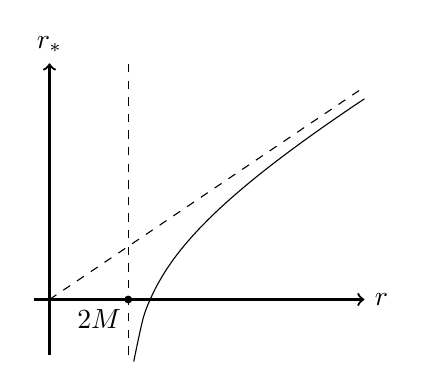
\begin{tikzpicture}
        \draw[thick,->] (0,-.7) -- (0,3) node[above] {\(r_*\)};
        \draw[thick,->] (-.2,0) -- (4,0) node[right] {\(r\)};
        \draw[domain=1.07:4,smooth,variable=\x] plot({\x},{(\x+ln(\x-1))/2});
        \draw[dashed] (0,0) -- (4,2.7);
        \draw[dashed] (1,-.7) -- (1,3);
        \fill (1,0) circle (0.05);
        \node[below] at (0.63,0) {\(2M\)};
    \end{tikzpicture}
\end{wrapfigure}
We have \(\dv{t}{r_*} = \pm1\), so \(t\mp r_*\) is a constant. Define \mbox{\(v = t + r_*\) (\(\dagger\))}, a constant along ingoing radial geodesics. The ingoing \emph{Eddington-Finklestein} coordinates are \(v,r,\theta,\phi\). In these coordinates, the line element is given by:
\begin{equation}
    \dd{s}^2 = - \left( 1-\frac{2M}{r} \right)\dd{v}^2 + 2\dd{v}\dd{r} + r^2\dd{\Omega}^2
\end{equation}
This is smooth for all \(r > 0\). In matrix form, the metric is:
\begin{equation}
    g_{\mu\nu} = 
    \begin{pmatrix}
        - \left( 1 - \frac{2M}{r} \right) & 1 & 0 & 0 \\
        1 & 0 & 0 & 0 \\
        0 & 0 & r^2 & 0 \\
        0 & 0 & 0 & r^2\sin^2\theta
    \end{pmatrix}
\end{equation}
We have \(g = \det g_{\mu\nu} = -r^4\sin^2\theta\), so \(g_{\mu\nu}\) is non-degenerate for all \(r > 0\) and furthermore it is Lorentzian for all \(r>0\).

In summary, spacetime can be extended through \(r=2M\) to a new region \(r<2M\).

Exercise: for \(0<r<2M\), define \(r_*\) by (\(*\)) and \(t\) by (\(\dagger\)). Show that the metrix in coordinates \(t,r,\theta,\phi\) is the Schwarzschild metric with \(0<r<2M\).

So for a ingoing radial null geodesic inside \(r=2M\) we have \(\dv{r}{\tau}=-1\), so it reaches \(r=0\) in finite \(\tau\).

Consider \(R_{abcd}R^{abcd}\). Some work will lead to:
\begin{equation}
    R_{abcd}R^{abcd} \propto \frac{M^2}{r^6} \rightarrow \infty \text{ as } r\rightarrow0
\end{equation}
This quantity is a scalar, so it diverges in any coordinate system. We call \(r=0\) a \emph{curvature singularity}. There are infinite tidal forces at \(r=0\). Note that \(r=0\) is not a part of the our spacetime, because \(g_{ab}\) is not defined there.

For \(r>2M\) we have the ``static'' KVF \(\pdv{t}\). In Eddington-Finklestein coordinates \(x^\mu\), we have:
\begin{equation}
    k = \pdv{x^\mu}{t}\pdv{x^\mu} = \pdv{v}
\end{equation}
Also, \(k^2 = g_{vv} = -\left( 1-\frac{2M}{r} \right)\), so \(k\) is null at \(r=2M\), and spacelike at \(r < 2M\). Only \(r > 2M\) is static.

\subsection{Finklestein diagram}
\lecture{22/01/16}
Consider outgoing radial null geodesics in \(r>2M\). We have \(t-r_*= \text{constant}\), so:
\begin{equation}
    v = 2r_* + \text{constant}
    = 2r + 4M\log\left|\frac{r}{2M}-1\right| + \text{constant}
    \tag{\(*\)}
    \label{sociable}
\end{equation}
Exercise: Consider null geodesics in ingoing Eddington-Finklestein coordinates and show that these fall into 2 families: ingoing with \(v = \text{constant}\), and outgoing either of the form \eqref{sociable} or \(r=2M\). 

Let \(t^*=v-r\). We can draw the radial null geodesics in a \emph{Finklestein diagram}:
\begin{figure}[H]
    \centering
    \begin{tikzpicture}
        \begin{scope}[thick, decoration={
            markings,
            mark=at position 0.5 with {\arrow{latex}}}
            ] 
            \clip (0,-3) rectangle (6,4);
            \begin{scope}[red]
                \draw[domain=3.07:6,smooth,variable=\x,postaction=decorate] plot({\x},{3*(ln(\x/3 - 1)+2)});
                \draw[domain=3.3:6,smooth,variable=\x,postaction=decorate] plot({\x},{3*(ln(\x/3 - 1)+1)});
                \draw[domain=3.6:6,smooth,variable=\x,postaction=decorate] plot({\x},{3*(ln(\x/3 - 1)+0.2)});

                \draw[domain=3.07:6,smooth,variable=\x,postaction=decorate] plot({6 - \x},{3*(ln(\x/3 - 1)+2)});
                \draw[domain=3.3:6,smooth,variable=\x,postaction=decorate] plot({6-\x},{3*(ln(\x/3 - 1)+1)});
                \draw[domain=3.6:6,smooth,variable=\x,postaction=decorate] plot({6-\x},{3*(ln(\x/3 - 1)+0.2)});
            \end{scope}
            \begin{scope}[blue]
                \draw[shift={(1,1)},postaction=decorate] (5.5,-10) -- (-6.5,4);
                \draw[shift={(2,2)},postaction=decorate] (5.5,-10) -- (-6.5,4);
                \draw[shift={(3,3)},postaction=decorate] (5.5,-10) -- (-6.5,4);
                \draw[shift={(4,4)},postaction=decorate] (5.5,-10) -- (-6.5,4);
                \draw[shift={(5,5)},postaction=decorate] (5.5,-10) -- (-6.5,4);
                \draw[shift={(6,6)},postaction=decorate] (5.5,-10) -- (-6.5,4);
            \end{scope}
        \end{scope}

        \draw[thick,->] (0,0) -- (6,0) node[right] {\(r\)};
        \draw[thick,->] (0,-3) -- (0,4) node[midway,above,sloped] {curvature singularity};
        \node[above] at (0,4) {\(t^*\)};
        \node[right,fill=white] at (3,-0.3) {\(2M\)};
        \draw[dashed, thick] (3,-3) -- (3,4);

        \node[right,rotate=-45, blue] at (6,2.5) {ingoing};
        \node[right,rotate=45, red] at (6,3) {outgoing};

        \newcommand{\lightcone}[4]{\
            \begin{scope}[shift={(#1,#2)}, scale=0.3, rotate=#4, semithick]
                \draw ({-sin(#3)},{-cos(#3)}) -- ({sin(#3)},{cos(#3)});
                \draw ({sin(#3)},{-cos(#3)}) -- ({-sin(#3)},{cos(#3)});
                \draw (0,{-cos(#3)}) ellipse ({sin(#3)} and {0.3*sin(#3)});
                \draw (0,{cos(#3)}) ellipse ({sin(#3)} and {0.3*sin(#3)});
            \end{scope}
        }

        \lightcone{2.6}{-0.1}{20}{23.5}
        \lightcone{1.98}{2.77}{10}{30}
        \lightcone{3.57}{0.93}{27}{15}
    \end{tikzpicture}
\end{figure}
In \(r < 2M\), \(r\) decreases along both families, and we reach \(r=0\) in finite \(\tau\). In fact we will show later that \(r\) decreases along \emph{any} timelike or null curve in \(r<2M\). Equipped with this knowledge we can make a rough definition of a \emph{black hole} as a region of space from which no signal can reach ``infinity''.

\subsection{Gravitational collapse}
The surface of a collapsing star follows a timelike geodesic, and we can plot this on a Finklestein diagram:
\begin{figure}[H]
    \centering
    \begin{tikzpicture}
        \begin{scope}[thick, shift={(-1,0)}, decoration={
            markings,
            mark=at position 0.5 with {\arrow{latex}}}
            ] 
            \clip (0,-3) rectangle (6,4);
            \begin{scope}[red]
                \draw[domain=3.07:9,smooth,variable=\x,postaction=decorate] plot({\x},{3*(ln(\x/3 - 1)+2)});
                \draw[domain=3.3:9,smooth,variable=\x,postaction=decorate] plot({\x},{3*(ln(\x/3 - 1)+1)});
                \draw[domain=3.6:9,smooth,variable=\x,postaction=decorate] plot({\x},{3*(ln(\x/3 - 1)+0.2)});

            \end{scope}
        \end{scope}

        \fill[gray!20] (0,-3) -- (0,3.5)
            .. controls (4,2.5) and (3.5,-2) .. (4,-3) -- cycle;

        \draw[thick,->] (0,0) -- (5,0) node[right] {\(r\)};
        \draw[thick,->] (0,-3) -- (0,4) node[midway,above,sloped] {curvature singularity};
        \node[above] at (0,4) {\(t^*\)};
        \node[right] at (2,-0.3) {\(2M\)};
        \draw[dashed, thick] (2,-3) -- (2,4);
        \draw (0,3.5) .. controls (4,2.5) and (3.5,-2) .. (4,-3);

        \draw[thick,<-] (3.3,-1.7) -- (4.2,-1.7) node[right]{stellar interior (not Schwarzschild)};
    \end{tikzpicture}
\end{figure}

It will be shown in the first example sheet that the total proper time along a timelike curve with \(r \le 2M\) can't exceed \(\pi M\), so a star collapses from \(r=2M\) to \(r=0\) within a proper time \(\pi M\) (this is about \SI{e-5}{\second} for \(M=M_{\astrosun}\). When this happens, a distant observer never sees the star cross \(r=2M\) -- it just redshifts away.

\subsection{Black hole region}
\begin{defn}
    A non-zero vector is \emph{causal} if it is timelike or null. A curve is \emph{causal} if its tangent vector is everywhere causal. 
\end{defn}
\begin{defn}
    A spacetime is \emph{time-orientable} if is admits a \emph{time orientation}, i.e.\ a causal vector field \(T^a\).
\end{defn}
\begin{defn}
    A \emph{future-directed} causal vector is one that lies in the same lightcone as the time orientation \(T^a\); a \emph{past-directed} causal vector is one that does not.
\end{defn}
Given a time orientation \(T^a\), we always have a second inequivalent time orientation \(-T^a\).

For \(r>2M\) Schwarzschild, the obvious choice of time orientation is \(k=\pdv{t}\). However, \(k=\pdv{v}\) is not causal for \(r<2M\). In ingoing Eddington-Finklestein coordinates, \(\pm\pdv{r}\) is null, since \(g_{rr} = 0\). We can choose either of these as a time orientation, but we want to pick a sign that agrees with \(k\) for \(r>2M\). We have:
\begin{equation}
    k\vdot\left( \pm \pdv{r} \right) = \pm g_{vr} = \pm 1
\end{equation}
Thus we use \(-\pdv{r}\) as the time orientation.

\begin{lemma}
    Let \(x^\mu(\lambda)\) be a future-directed causal curve. If \(r(\lambda_0) \le 2M\), then \(r(\lambda) \le 2M\) for all \(\lambda \ge \lambda_0\).
\end{lemma}
\begin{proof}
    Let \(V^\mu = \dv{x^\mu}{\lambda}\). \(V^\mu\) is future-directed. Thus we have:
    \begin{align}
        0 \le \left( -\pdv{r} \right)\vdot V = -g_{r\mu}V^\mu = -V^v = - \dv{v}{\lambda}
    \end{align}
    and so:
    \begin{align}
        & V^2 = -\left(1-\frac{2M}{r}\right) \left( \dv{v}{\lambda} \right)^2 + 2 \dv{v}{\lambda}\dv{r}{\lambda} + r^2 \left( \dv{\Omega}{\lambda} \right)^2 \\
        \implies & -2\dv{v}{\lambda}\dv{r}{\lambda} = \underbrace{-V^2}_{\ge0} - \left( 1-\frac{2M}{r} \right)\left( \dv{v}{\lambda} \right)^2 + \underbrace{r^2\left( \dv{\Omega}{\lambda} \right)^2}_{\ge0}
    \end{align}
    Thus if \(r \le 2M\), we have \(\dv{v}{\lambda}\dv{r}{\lambda}\le0\). 
    
    Suppose \(r \le 2M\) and \(\dv{r}{\lambda} > 0\). Then since \(\dv{v}{\lambda}\le 0\) we must have \(\dv{v}{\lambda} = 0\), and hence \(V^2 = 0 = \dv{\Omega}{\lambda}\). The only non-zero component of \(V\) is \(V^r = \dv{r}{\lambda}>0\), so \(V\) is a positive multiple of \(\pdv{r}\), but this implies that \(V\) is past-directed, which is a contradiction.

    Hence we have \(\dv{r}{\lambda} \le 0\) if \(r \le 2M\), and we can show similarly \(\dv{r}{\lambda} < 0\) if \(r < 2M\). Hence if \(r(\lambda_0) < 2M\), then \(r(\lambda)\) is monotonically decreasing for \(\lambda \ge \lambda_0\). \disapprove
\end{proof} 

\subsection{Detecting black holes}
Black holes have two recognizable qualities:
\begin{itemize}
    \item Unlike in the case of cold stars, there is no upper bound on the mass of a black hole.
    \item Black holes are very small for a given mass.
\end{itemize}

One interesting case is that of the \emph{supermassive black holes}. No one knows how they form...

\subsection{Orbits around black holes}
\lecture{25/01/16}
Comsider timelike geodesics, and recall the orbital equation of a Schwarzschild black hole:
\begin{equation}
    \frac{1}{2}\left( \dv{r}{\tau} \right)^2 + V(r) = \frac{1}{2}E^2
    \qq{where}
    V(r) = \frac{1}{2}\left( 1-\frac{2M}{r} \right)\left( 1 + \frac{h^2}{r^2} \right)
\end{equation}
It can easily be shown that \(V'(r)=0\) if \(r = r_\pm = \frac{h^2\pm\sqrt{h^4-12h^2M^2}}{2M}\). Lets plot \(V\):

\begin{figure}[H]
    \centering
    \begin{tikzpicture}
        \draw[->, thick] (0,0) -- (6,0) node[right] {\(r\)};
        \draw[->, thick] (0,-1) -- (0,4) node[above] {\(V\)};
        \draw (0.5,-1) .. controls (0.7,0) and (1,3.5) .. (2,3.5)
            .. controls (2.5,3.5) and (3,2.5) .. (3.5,2.5)
            .. controls (4,2.5) and (4,2.9) .. (6,2.95);
        \draw[dashed] (0,3) node[left] {\(\frac{1}{2}\)} -- (6,3);
        \draw[dashed] (2,0) node[below] {\(r_-\)} -- (2,3.5);
        \draw[dashed] (3.5,0) node[below] {\(r_+\)} -- (3.5,2.5);

        \node[right] at (7.5,2.25) {\(r=r_+\) is a stable circular orbit};
        \node[right] at (7.5,1.75) {\(r=r_-\) is an unstable circular orbit};
    \end{tikzpicture}
\end{figure}
It is a simple exercise to show that \(3M < r_- < 6M < r_+\). We call \(r=6M\) the \emph{innermost stable circular orbit} (ISCO).

Suppose \(r=r_\pm\), then we have a circular orbit \(\dv{r}{\tau} = 0\), and we can show:
\begin{equation}
    \frac{E^2}{2}=V(r) \implies E = \frac{r-2M}{r^{\frac{1}{2}}(r-3M)^{\frac{1}{2}}} \approx 1 - \frac{M}{2r} \text{ for } r\gg2M
\end{equation}
Hence we have that the energy of a distant orbit is approximately \(m-\frac{Mm}{2r}\). \(m\) is the rest mass energy of the orbiting particle, and \(\frac{Mm}{2r}\) is the gravitational binding energy of its orbit.

\begin{wrapfigure}{r}{0.4\linewidth}
    \centering
    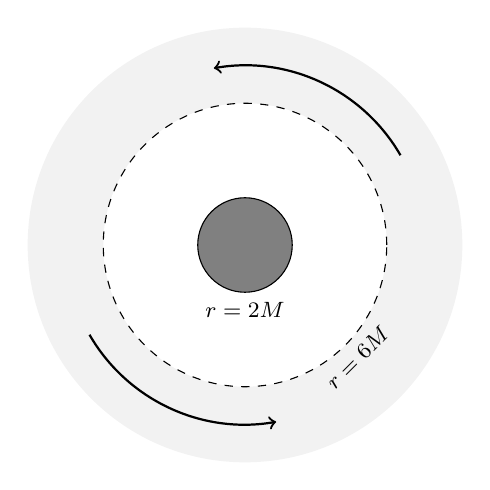
\begin{tikzpicture}[scale=1.2]
        \fill[gray!10] (0,0) circle (2.3);
        \fill[white] (0,0) circle (1.5);
        \fill[gray] (0,0) circle (0.5);
        \draw (0,0) circle (0.5);
        \draw[dashed] (0,0) circle (1.5);

        \draw[thick,->] ({1.9*cos(30)},{1.9*sin(30)}) arc (30:100:1.9);
        \draw[thick,->] ({1.9*cos(-150)},{1.9*sin(-150)}) arc (-150:-80:1.9);

        \node[below,rotate=45] at ({1.5*cos(45)},{-1.5*sin(45)}) {\footnotesize\(r=6M\)};
        \node[below] at (0,-0.5) {\footnotesize\(r=2M\)};
    \end{tikzpicture}
\end{wrapfigure}
When a star orbits around a black hole, the black hole robs the star of matter, forming an \emph{accretion disc} around the black hole. As a first approximation we will assume that particles in this accretion disc follow stable circular orbits of the form above. Friction between the particles causes their \(E\) to decrease, and hence their \(r\) to also decrease, and so these particles will fall towards the ISCO, where they will then fall into the black hole.

At \(r\to\infty\) we have \(E = 1\), and at the ISCO we have \(E=\sqrt{\frac{8}{9}}\). Thus the proportion of lost to friction (and then radiated away as x-rays) is \(1-\sqrt{\frac{8}{9}}\approx6\%\).

\subsection{White holes}
Consider again the region \(r>2M\), and let \(u = t-r_*\). We define the \emph{outgoing} Eddington-Finklestein coordinates as \(u,r,\theta,\phi\). In these coordinates, the line element is given by:
\begin{equation}
    \dd{s}^2=-\left( 1 - \frac{2M}{r} \right)\dd{u}^2-2\dd{u}\dd{r} + r^2\dd{\Omega}^2
\end{equation}
Since \(g_{\mu\nu}\) is smooth and \(\det g \ne 0\) for all \(r>0\), we can extend this to \(0 < r \le 2M\), and again we have a curvature singularity at \(r=0\). However it is important to note that this is not the same \(r < 2M\) region as before! To see this, consider outgoing radial null geodesics which have \(u\) constant and \(\dv{r}{\tau} = +1\). These have \(r\) increasing through \(r=2M\), in direct contradiction with the previous case. \(r < 2M\) is \emph{not} a black hole.

Exercise: show (i) \(k=\pdv{u}\), (ii) the time orientation equivalent to \(k\) for \(r\gg2M\) is \(+\pdv{r}\).

\(r<2M\) is known as a \emph{white hole region}; it is a region into which no signal from infinity can enter. In a certain sense a white hole is the time reversal of a black hole: \(u\mapsto -v\) is an isometry mapping outgoing Eddington-Finklestein coordinates to ingoing Eddington-Finklestein coordinates, but it does not preserve the time-orientation.

\subsection{Kruskal extension}
Consider \(r>2M\) Schwarzschild spacetime. We define \emph{Kruskal-Szekeres} coordinates \((U,V,\theta,\phi)\) by
\begin{equation}
    U = -e^{-u/4M} < 0
    \qq{and}
    V = e^{v/4M} > 0.
\end{equation}
We have
\begin{equation}
    UV = -e^{r_*/2M} = - e^{r/2M}\left( \frac{r}{2M} - 1 \right),
    \tag{\(**\)}
    \label{uv}
\end{equation}
which is monotonic and thus determines \(r = r(U,V)\). Similarly, 
\begin{equation}
    \frac{V}{U} = -e^{t/2M}
\end{equation}
determines \(t = t(U,V)\).

Exercise: show that the metric in Kruska-Szekeres coordinates is given by
\begin{equation}
    \dd{s}^2 = -\frac{32M^3e^{-r(U,V)/2M}}{r(U,V)} \dd{U}\dd{V} + r(U,V)^2 \dd{\Omega}^2.
\end{equation}
We use \eqref{uv} to define \(r(U,V)\) for \(U\ge0\) or \(V\le0\). We can analytically extend the spacetime with \(\det g \ne0\) through \(U=0\) or \(V=0\) to new regions with \(U\ge0\) or \(V\le0\). \(r=2M\) corresponds to two surfaces \(U=0\) and \(V=0\), intersecting at \(U=V=0\). \(r=0\) corresponds to a hyperbola with 2 branches. Ingoing and outgoing geodesics are described by \(V\), \(U\) constant respectively. We can plot thse features on a \emph{Kruskal diagram}:

\begin{figure}[H]
    \centering
    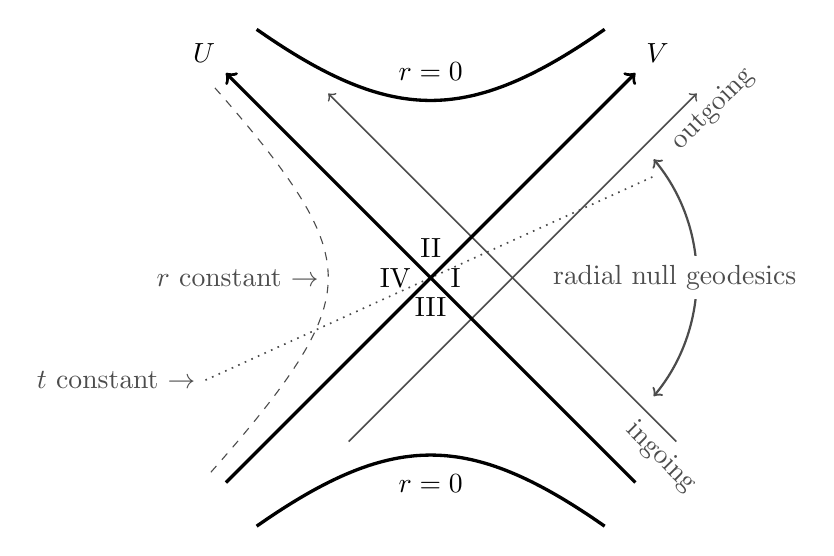
\begin{tikzpicture}[scale=1.3]
        \begin{scope}[black!70]
            \draw[domain=-1.9:1.9,smooth,variable=\x,dashed] plot({-sqrt(1+\x*\x))},{\x});
            \node[left] at (-1,0) {\(r\) constant \(\rightarrow\)};

            \draw[dotted, semithick] (-2.2,-1) -- (2.2,1) node[left, at start] {\(t\) constant \(\rightarrow\)};

            \draw[semithick, <-] (-1,1.8) -- (2.4,-1.6) node[below, at end, sloped] {ingoing};
            \draw[semithick, <-] (2.6,1.8) -- (-0.8,-1.6) node[below, at start, sloped] {outgoing};
            \draw[thick, ->] (2.6,0) arc (0:40:1.8);
            \draw[thick, ->] (2.6,0) arc (0:-40:1.8);
            \node[right, fill=white] at (1.1,0) {radial null geodesics};
        \end{scope}

        \draw (0.1,0) node[right] {I};
        \draw (0,0.1) node[above] {II};
        \draw (0,-0.1) node[below] {III};
        \draw (-0.1,0) node[left] {IV};

        \draw[domain=-1.7:1.7,smooth,variable=\x,very thick] plot({\x},{sqrt(3+\x*\x))});
        \node[above] at (0,{sqrt(3)+0.1}) {\(r=0\)};
        \draw[domain=-1.7:1.7,smooth,variable=\x,very thick] plot({\x},{-sqrt(3+\x*\x))});
        \node[below] at (0,{-sqrt(3)-0.1}) {\(r=0\)};

        \draw[very thick,->] (-2,-2) -- (2,2) node[above right] {\(V\)};
        \draw[very thick,->] (2,-2) -- (-2,2) node[above left] {\(U\)};
    \end{tikzpicture}
\end{figure}

Note that points in this diagram correspond to \(U=V=\) constant two dimensional surfaces in space.

There are four regions on the Kruskal diagram:
\begin{enumerate}[label=\Roman*:]
    \item This is just the \(r > 2M\) Schwarzschild spacetime that we are used to.
    \item This is the black hole region of ingoing Eddington-Finklestein coordinates.
    \item This is the white hole region of outgoing Eddington-Finklestein coordinates.
    \item This is new; it is an asymptotically flat region isometric to region I.
\end{enumerate}

Exercise: show
\begin{equation}
    k= \frac{1}{4M}\left(V\pdv{V} - U\pdv{U}\right) \qq{and} k^2 = - \left(1-\frac{2M}{r}\right).
\end{equation}
Thus \(k\) is timelike in regions I and IV, spacelike in II and III, and null at \(V=0\) or \(U=0\). We can plot its integral curves:

\begin{figure}[H]
    \centering
    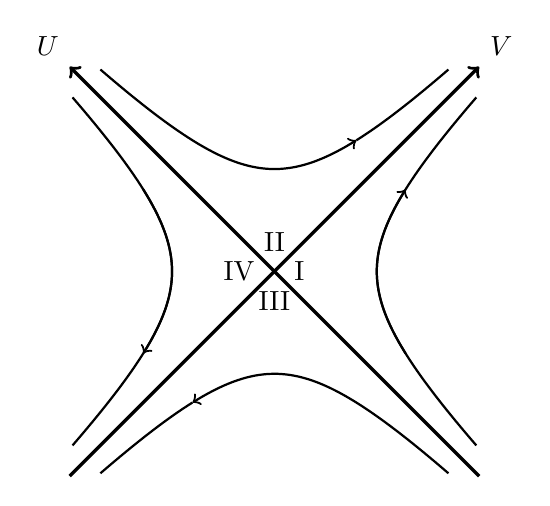
\begin{tikzpicture}[scale=1.3]
        \draw (0.1,0) node[right] {I};
        \draw (0,0.1) node[above] {II};
        \draw (0,-0.1) node[below] {III};
        \draw (-0.1,0) node[left] {IV};

        \draw[domain=-1.7:0.8,smooth,variable=\x,thick,->] plot({\x},{sqrt(1+\x*\x))});
        \draw[domain=0.8:1.7,smooth,variable=\x,thick] plot({\x},{sqrt(1+\x*\x))});

        \draw[domain=-1.7:0.8,smooth,variable=\x,thick,->] plot({-\x},{-sqrt(1+\x*\x))});
        \draw[domain=0.8:1.7,smooth,variable=\x,thick] plot({-\x},{-sqrt(1+\x*\x))});

        \draw[domain=-1.7:0.8,smooth,variable=\x,thick,->] plot({sqrt(1+\x*\x))},{\x});
        \draw[domain=-0.8:1.7,smooth,variable=\x,thick] plot({sqrt(1+\x*\x))},{\x});

        \draw[domain=-1.7:0.8,smooth,variable=\x,thick,->] plot({-sqrt(1+\x*\x))},{-\x});
        \draw[domain=-0.8:1.7,smooth,variable=\x,thick] plot({-sqrt(1+\x*\x))},{-\x});

        \draw[very thick,->] (-2,-2) -- (2,2) node[above right] {\(V\)};
        \draw[very thick,->] (2,-2) -- (-2,2) node[above left] {\(U\)};
    \end{tikzpicture}
\end{figure}

\(U=0\) and \(V=0\) are both independently fixed by \(k\). \(k=0\) on \(U=V=0\), a region known as the \emph{bifurcation 2-sphere}.

\lecture{27/01/16}
\subsection{Einstein-Rosen bridge}
Consider a constant \(t\) slice of \emph{Kruskal} spacetime. We define the coordinate \(\rho\) on this slice by
\begin{equation}
    r=\rho+M+\frac{M^2}{4\rho} \qq{such that} \rho>\frac{M}{2} \;\text{in I},\; \rho<\frac{M}{2} \; \text{in IV.}
\end{equation}
In \emph{isotropic coordinates} \((t,\rho,\theta,\phi)\), the line element is
\begin{equation}
    \dd{s}^2 = - \frac{\left(1-\frac{M}{2\rho}\right)^2}{\left(1+\frac{M}{2\rho}\right)^2} \dd{t}^2 + \left(1+\frac{M}{2\rho}\right)^4 (\dd{\rho}^2+\rho^2\dd{\Omega}^2).
\end{equation}
Note that \(\rho\to\frac{M^2}{4\rho}\) interchanges I and IV.

\begin{wrapfigure}{r}{0.4\linewidth}
    \centering
    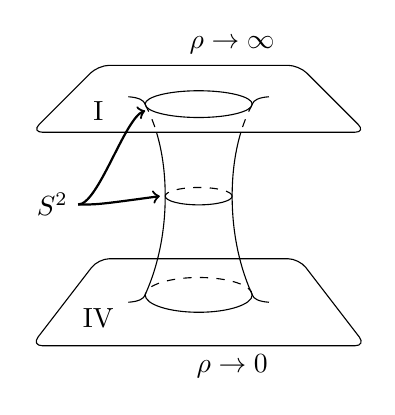
\begin{tikzpicture}[scale=0.85]
        \draw[rounded corners, shift={(0,0.08)}] (0,3) -- (5,3) -- (4,4) -- (1,4) -- cycle;
        \draw[rounded corners, shift={(0,-0.11)}] (0,0) -- (5,0) -- (4,1.3) -- (1,1.3) -- cycle;

        \draw (2.5,3.5) ellipse (0.8 and 0.2);
        \begin{scope}[shift={(0,2.125)},yscale=0.26]
            \draw (3,0) arc (0:-180:0.5);
            \draw[dashed] (3,0) arc (0:180:0.5);
        \end{scope}
        \begin{scope}[shift={(0,0.65)},yscale=0.325]
            \draw (3.3,0) arc (0:-180:0.8);
            \draw[dashed] (3.3,0) arc (0:180:0.8);
        \end{scope}
        
        \begin{scope}
            \clip[shift={(0,0.08)}] (0,3) rectangle (5,0);
            \draw (3.3,3.5) .. controls (3.28,3.44) and (3,3) .. (3,2.125)
                            .. controls (3,1.25) and (3.28,0.71) .. (3.3,0.65);
            \draw (1.7,3.5) .. controls (1.72,3.44) and (2,3) .. (2,2.125)
                            .. controls (2,1.25) and (1.72,0.71) .. (1.7,0.65);
        \end{scope}
        \begin{scope}[dashed]
            \clip[shift={(0,0.08)}] (0,3) rectangle (5,4);
            \draw (3.3,3.5) .. controls (3.28,3.44) and (3,3) .. (3,2.125)
                            .. controls (3,1.25) and (3.28,0.71) .. (3.3,0.65);
            \draw (1.7,3.5) .. controls (1.72,3.44) and (2,3) .. (2,2.125)
                            .. controls (2,1.25) and (1.72,0.71) .. (1.7,0.65);
        \end{scope}

        \draw (3.3,3.5) .. controls (3.32,3.56) and (3.4,3.6) .. (3.55,3.61);
        \draw (1.7,3.5) .. controls (1.68,3.56) and (1.6,3.6) .. (1.45,3.61);
        \draw (3.3,0.65) .. controls (3.32,0.59) and (3.4,0.55) .. (3.55,0.54);
        \draw (1.7,0.65) .. controls (1.68,0.59) and (1.6,0.55) .. (1.45,0.54);

        \node at (1,3.4) {I};
        \node at (1,0.3) {IV};

        \draw[->, thick] (0.7,2) node[left] {\(S^2\)} .. controls (1,2) and (1.4,3.3) .. (1.7,3.4);
        \draw[->, thick] (0.7,2) .. controls (1,2) .. (1.92,2.125);

        \node[above] at (3,4.1) {\(\rho\to\infty\)};
        \node[below] at (3,-0.1) {\(\rho\to0\)};
    \end{tikzpicture}
\end{wrapfigure}
On a constant \(t\) surface, the induced metric is
\begin{equation}
    \dd{s}^2 = \left(1+\frac{M}{2\rho}\right)^4 (\dd{\rho}^2+\rho^2\dd{\Omega}^2).
\end{equation}
If we take \(\rho>0\), we see that the surface is a Riemannian manifold with topology \(\RR\times S^2\). We can visualise this surface by embedding into four dimensional Euclidean space.
We have two asymptotically flat regions at \(\rho\to\infty\), \(\rho\to0\) connected by a ``throat'' with minimum radius \(r=2M\) at \(\rho = \frac{M}{2}\).

\subsection{Extendability and singularities}
\begin{defn}
    A spacetime \((\mathcal{M},g)\) is said to be \emph{extendable} if it is isometric to a proper subset of another spacetime \((\mathcal{M}',g)\), called an \emph{extension} of \((\mathcal{M},g)\).
\end{defn}
\begin{eg}
    \(r>2M\) Schwarzschild spacetime is extendable, with for example Kruskal spacetime as an extension. The isometry in question is the identity map.
    Kruskal spacetime on the other hand is inextendible, and is in fact a \emph{maximal analytic extension} of \((\mathcal{M},g)\).
\end{eg}

There are many types of singularities.
\begin{itemize}
    \item A \emph{scalar curvature singularity} is a region in which a scalar constructed from the Riemann tensor \(R_{abcd}\) blows up.
    \item More generally, a \emph{curvature singularity} is a region in which there does not exist a chart such that the components of the Riemann tensor \(R_{\mu\nu\rho\sigma}\) are finite.
    \item It is possible to have singularities which have nothing to do with the curvature tensor. For example consider \(\mathcal{M}=\RR^2\) with polar coordinates \((r,\phi)\), where we identify \(\phi \sim \phi+2\pi\), with line element given by
        \begin{equation}
            \dd{s}^2=\dd{r}^2+\lambda^2r^2\dd{\phi}^2
        \end{equation}
        for some constant \(\lambda>0\). There are two cases:
        \begin{itemize}
            \item In the case \(\lambda=1\), this is just Euclidean space, and \(r=0\) is just a coordinate singularity.
            \item If \(\lambda\ne1\), then set \(\phi'=\lambda\phi\) to obtain
                \begin{equation}
                    \dd{s}^2 = \dd{r}^2+r^2\dd{\phi'}^2.
                \end{equation}
                Locally, this is isometric to Euclidean space. It is flat, so \(R_{abcd}=0\) and there is no curvature singularity. However the range of the angular coordinate has changed; our identification has changed to \(\phi'\sim\phi+2\pi\lambda\). Consider a circle with \(r=\epsilon\). The ratio of the circumference to the radius of this circle is \(2\pi\lambda\epsilon/\epsilon=2\pi\lambda\). As we take \(\epsilon\), we would expect this ratio to approach \(2\pi\) if the geometry were locally flat at \(r=0\), but this is not the case. \(g\) is not smooth at \(r=0\). This type of singularity is called a \emph{conical singularity}.
        \end{itemize}
\end{itemize}

\begin{defn}
    \(p\in\mathcal{M}\) is a \emph{future endpoint} of a future-directed causal curve \(\gamma:(a,b)\to\mathcal{M}\) if for any neighbourhood \(\mathcal{O}\) of \(p\) there exists a \(t_0\) such that \(\gamma(t)\in\mathcal{O}\) for all \(t>t_0\). We say \(\gamma\) is \emph{future-inextendable} if it has no future endpoint.
\end{defn}

\begin{eg}
    Let \((\mathcal{M},g)\) be Minkowski space, and \(\gamma:(-\infty,0)\to\mathcal{M}\), \(\gamma(t)=(t,0,0,0)\). Then \((0,0,0,0)\) is a future end point of \(\gamma\). If however \((\mathcal{M},g)\) is Minkowski\(\setminus(0,0,0,0)\), then \(\gamma\) is future-inextendable.
\end{eg}

\begin{defn}
    A geodesic is \emph{complete} if an affine parameter extends to \(\pm\infty\). A spacetime is \emph{geodesically complete} if all inextendable geodesics are complete. If a spacetime is both inextendable and geodesically incomplete, then we say it is \emph{singular}.
\end{defn}

\section{The Initial Value Problem}
\subsection{Predictability}
\begin{defn}
    A \emph{partial Cauchy surface} \(\Sigma\) is a hypersurface for which no two points are connected by a causal curve in \(\mathcal{M}\).
\end{defn}
\begin{defn}
    The \emph{future domain of dependence} of \(\Sigma\) is the set 
    \begin{equation}
        D^+(\Sigma) = \{p\in\mathcal{M}\;\st\;\text{every past-inextendible causal curve through \(p\) intersects \(\Sigma\)}\}.
    \end{equation}
    We define the \emph{past domain of dependence} \(D^-(\Sigma)\) in a similar way. The \emph{domain of dependence} is \(D(\Sigma) = D(\Sigma^+)\cup D(\Sigma^-)\).
\end{defn}

A causal geodesic in \(D(\Sigma)\) is uniquely determined by its velocity at \(q\in\Sigma\) (this is because the geodesic equation is a hyperbolic PDE).

\begin{eg}
    Consider 2d Minkowski space, and the surface \(\Sigma = \{(0,x)\st x>0\}\). Then \(D^+(\Sigma)= \{(t,x)\st 0 \le t < x\}\), \(D^-(\Sigma)= \{(t,x)\st -x < t \le 0\}\).
\end{eg}

\begin{defn}
    \((\mathcal{M},g)\) is called \emph{globally hyperbolic} if it contains a \emph{Cauchy surface} i.e.\ a partial Cauchy surface whose domain of dependence is all of \(\mathcal{M}\).
\end{defn}

\begin{eg}
    Minkowsi spacetime is globally hyperbolic (for instance \(t\) constant is a Cauchy surface). Kruskal spacetime is globally hyperbolic (for instance \(U+V\) constant is a Cauchy surface).

    2d Minkowski spacetime with \((0,0)\) removed is \emph{not} globally hyperbolic.
\end{eg}

\begin{theorem}
    Suppose \((\mathcal{M},g)\) is a globally hyperbolic spacetime. Then:
    \begin{enumerate}
        \item There exists a \emph{global time function} i.e.\ a map \(t:\mathcal{M}\to\RR\) such that \((\dd{t})^a\) is future-directed and timelike.
        \item \(t\) constant surfaces are Cauchy and all have the same topology \(\Sigma\).
        \item \(\mathcal{M} = \RR\times\Sigma\).
    \end{enumerate}
\end{theorem}

Exercise: show \(U+V\) is a global time function for Kruskal spacetime. \(U+V = 0\) is an Einstein-Rosen bridge, so \(\Sigma = \RR \times S^2\) and \(\mathcal{M} = \RR^2\times S^2\).


\begin{wrapfigure}{r}{0.4\linewidth}
    \centering
    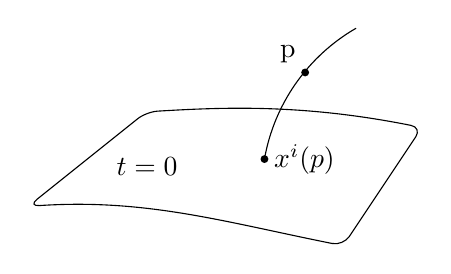
\begin{tikzpicture}
        \draw[rounded corners] (0,0) .. controls (1.5,0.1) and (2.5,-0.2) .. (4,-0.5)
                                     -- (5, 1)
                                     .. controls (3.5, 1.3) and (2.5,1.26) .. (1.5,1.2)
                                     -- cycle;
        \draw (3,0.6) arc (170:120:2.4);
        \fill (3,0.6) circle (0.05) node[right] {\(x^i(p)\)};
        \fill (3.517,1.7) circle (0.05) node [above left] {p};
        \node[right] at (1,0.5) {\(t=0\)};
    \end{tikzpicture}
\end{wrapfigure}
If we have a time function \(t\), we will often carry out a \emph{3+1 split} to obtain a set of local coordinates. Suppose we have coordinates \(x^i\) on the surface \(t=0\), and a timelike vector field \(T^a\).
For a point \(p\) near \(t=0\), we let \(x_i(p)\) be the coordinate of the point where the integral curve of \(T^a\) through \(p\) intersects \(t=0\). Thus we have a coordinate chart \(t,x^i\). In these coordinates, the metric is given by
\begin{equation}
    \dd{s}^2 = -N(t,x)^2\dd{t}^2 + h_{ij}(t,x)(\dd{x^i} + N^i(t,x)\dd{t})(\dd{x^j} + N^j(t,x)\dd{t}),
\end{equation}
where \(N\) and \(N^i\) are known as the \emph{lapse function} and \emph{shift vector} respectively, and \(h_{ij}\) is the metric on a constant \(t\) surface.

\subsection{Initial value problem in GR}
\lecture{29/01/16}
We can view the Einstein equations as an initial value problem. We are given \(\Sigma\), a 3d Riemannian manifold with metric \(h_{ab}\) and extrinsic curvature \(K_{ab}\). In addition we have the \emph{Hamiltonian constraint}
\begin{equation}
    R' - K^{ab}K_{ab} + K^2 = 16\pi\rho,
\end{equation}
where \(R'\) is the Ricci scalar of \(h\), \(K=K\indices{_a^a}\) and \(\rho = T_{ab}n^an^b\) (with \(n\) a unit normal to \(\Sigma\)), and the \emph{momentum constraint}
\begin{equation}
    D_bK\indices{^b_a} - D_aK = 8\pi h\indices{_a^b}T_{bc}n^c,
\end{equation}
where \(D_b\) is the Levi-Civita connection with regard to \(h\).

\begin{theorem}[Choquet-Bruhat and Geroch 1969]
    Given initial data satisfying vacuum constraints (i.e.\ the right hand sides of the above equal to 0), there exists a unique (up to diffeomorphism) spacetime \(\mathcal{M},g\), known as the \emph{maximal Cauchy development} of \(\Sigma, h_{ab}, K_{ab}\), such that the following are satisfied:
    \begin{enumerate}
        \item \((\mathcal{M},g)\) obeys the vacuum Einstein equations.
        \item \((\mathcal{M},g)\) is globally hyperbolic with Cauchy surface \(\Sigma\).
        \item The induced metric and extrinsic curvature of \(\Sigma\) are \(h_{ab}\) and \(K_{ab}\) respectively.
        \item Any other spacetime obeying 1-3 is isometric to a subset of \((\mathcal{M},g)\).
    \end{enumerate}
\end{theorem}
Note that \((\mathcal{M},g)\) may be extendable, but the solution will be non-unique outside of \(D(\Sigma)\).
\begin{eg}
    Consider \(\Sigma = \{(x,y,z)\st x>0\}\), \(h_{\mu\nu} = \delta_{\mu\nu}\), \(K_{\mu\nu} = 0\). Then \((\mathcal{M},g)\) is the region of Minkowski spacetime with \(|t|<x\), and this is clearly extendable.
\end{eg}
In the preceding example, \((\mathcal{M},g)\) was extendable because \((\Sigma, h_{ab})\) was extendable, but this need not be the case.
\begin{eg}
    Consider \(M<0\) Schwarzschild. The metric is
    \begin{equation}
        \dd{s}^2 = - \left(1+\frac{2|M|}{r}\right)\dd{t}^2 + \left(1+\frac{2|M|}{r}\right)^{-1}\dd{r}^2 + r^2\dd{\Omega}^2.
    \end{equation}
    There is a curvature singularity at \(r=0\) but, unlike the positive mass case, there is no event horizon. We choose the initial data \((\Sigma,h_{ab},K_{ab})\) to be that given by the surface \(t=0\); this is inextendable (but not geodesically complete since it is singular at \(r=0\)). For outgoing radial null geodesics at small \(r\), we have 
    \begin{equation}
        \pdv{t}{r} = \left(1+\frac{2|M|}{r}\right)^{-1} \approx \frac{r}{2|M|},
    \end{equation}
    so we can write \(t \approx t_0 + \frac{r^2}{4|M|}\). If \(t_0>0\) then the geodesic never intersects \(\Sigma\), so \(\Sigma\) is not a Cauchy surface for \(\mathcal{M}\). The boundary of \(D(\Sigma)\) is given by those geodesics with \(t_0=0\).
    \begin{figure}[H]
        \centering
        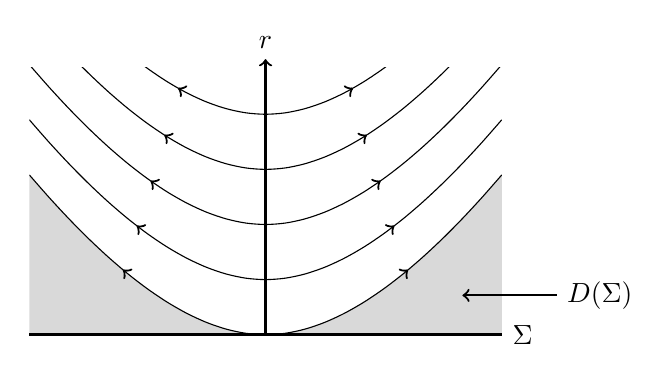
\begin{tikzpicture}
            \fill[gray!30, domain=-3:3,smooth,variable=\x] plot({\x},{1.5*abs(\x)*(1-exp(-0.2*abs(\x)))}) -- (3,0) -- (-3,0) -- cycle;

            \begin{scope}
                \clip (-3,0) rectangle (3,3.4);
                \foreach \tz in {0,0.7,1.4,2.1,2.8}
                {
                    \draw[domain=-3:3,smooth,variable=\x] plot({\x},{\tz+1.5*abs(\x)*(1-exp(-0.2*abs(\x)))});
                    \draw[thick, ->] (1.8-\tz/4,{\tz+1.5*(1.8-\tz/4)*(1-exp(-0.2*(1.8-\tz/4)))}) 
                        -- (1.81-\tz/4,{\tz+1.5*(1.81-\tz/4)*(1-exp(-0.2*(1.81-\tz/4)))});
                    \draw[thick, ->] (-1.8+\tz/4,{\tz+1.5*(1.8-\tz/4)*(1-exp(-0.2*(1.8-\tz/4)))}) 
                        -- (-1.81+\tz/4,{\tz+1.5*(1.81-\tz/4)*(1-exp(-0.2*(1.81-\tz/4)))});
                }
            \end{scope}

            \draw[thick,->] (0,0) -- (0,3.5) node[above] {\(r\)};
            \draw[very thick] (-3,0) -- (3,0) node[right] {\(\Sigma\)};

            \draw[thick,<-] (2.5,0.5) -- (3.7,0.5) node [right] {\(D(\Sigma)\)};
        \end{tikzpicture}
    \end{figure}
    The solution outside of \(D(\Sigma)\) is \emph{not} determined by the data on \(\Sigma\); in particular, it need not be the negative mass Schwarzschild that we started with.
\end{eg}
This time, the maximal development was extendable because the initial data was singular, but again this is not necessary.
\begin{eg}
    Consider 4d Minkowski spacetime, and start with data on the surface \(\Sigma = \{-t^2+x^2+y^2+z^2 = -1, t < 0\}\). This is one sheet of a hyperboloid. The maximal development of \(\Sigma\) is the interior of the past lightcone of the origin, and this is extendable.
    \begin{figure}[H]
        \centering
        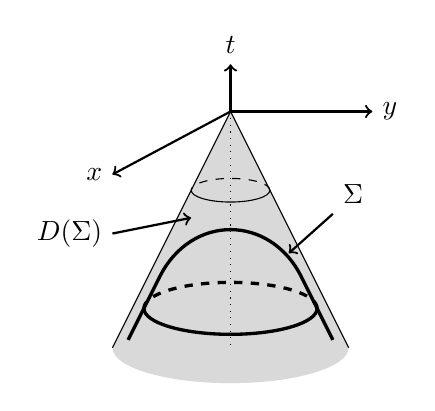
\begin{tikzpicture}
            \fill[gray!30,yscale=0.3] (0,0) -- (1.5,-10) arc (0:-180:1.5) -- cycle;

            \draw[thick,->] (0,0) -- (0,0.6) node[above] {\(t\)};
            \draw[thick,->] (0,0) -- (1.8,0) node[right] {\(y\)};
            \draw[thick,->] (0,0) -- (-1.5,-0.8) node[left] {\(x\)};

            \draw[dotted] (0,0) -- (0,-3);

            \draw (0,0) -- (1.5,-3);
            \draw (0,0) -- (-1.5,-3);
            \draw[shift={(0.5,-1)},yscale=0.3] (0,0) arc (0:-180:0.5);
            \draw[shift={(0.5,-1)},yscale=0.3, dashed] (0,0) arc (0:180:0.5);

            \draw[very thick] (1.3,-2.9) -- (0.9,-2.1)
                .. controls (0.5,-1.3) and (-0.5,-1.3)
                .. (-0.9,-2.1) -- (-1.3,-2.9);

            \draw[very thick, shift={(1.1,-2.5)},yscale=0.3] (0,0) arc (0:-180:1.1);
            \draw[very thick, shift={(1.1,-2.5)},yscale=0.3, dashed] (0,0) arc (0:180:1.1);

            \draw[thick, <-] (0.74,-1.8) -- (1.3,-1.3) node[above right] {\(\Sigma\)};
            \draw[thick, <-] (-0.5, -1.35) -- (-1.5,-1.55) node [left] {\(D(\Sigma)\)};
        \end{tikzpicture}
    \end{figure}
\end{eg}
Now, the maximal development is extendible because the initial data is ``asymptotically null''. To avoid this problem, we will use asymptotically flat initial data.

\begin{defn}
    \((\Sigma,h_{ab},K_{ab})\) is an \emph{asymptotically flat end} if:
    \begin{itemize}
        \item \(\Sigma\) is diffeomorphic to \(\RR^3\setminus B\) where \(B\) is a closed ball centred on the origin in \(\RR^3\).
        \item If we pull back \(\RR^3\) coordinates to give coordinates \(x^i\) on \(\Sigma\), then the metric is \(h_{ij} = \delta_{ij} + O(1/r)\) and the extrinsic curvature is \(K_{ij} = O(1/r^2)\).
        \item \(h_{ij,k} = O(1/r^2)\) etc.
    \end{itemize}
\end{defn}

\begin{defn}
    A set of initial data is said to be \emph{asymptotically flat with \(N\) ends} if it is a union of a compact set with \(N\) asymptotically flat ends.
\end{defn}

\begin{eg}
    Consider \(M>0\) Schwarzschild spacetime. \(\Sigma = \{t = \text{constant}, r>2M\}\) is an asymptotically flat end. \(\Sigma\) is part of an Einstein-Rosen bridge, which is asymptotically flat with 2 ends (in fact it is the union of two copies of \(\Sigma\) and the bifurcation two-sphere at \(r=2M\)).
\end{eg}

\subsection{Strong cosmic censorship}
The strong cosmic censorship conjecture (by Penrose) is the following:
\begin{quote}
    Given vacuum initial data \((\Sigma,h_{ab},K_{ab})\) that is geodesically complete and asymptotically flat, then  generically the maximal Cauchy development is inextendable.
\end{quote}
The conjecture has been shown to be true for nearly flat data, but there are non-generic counterexamples.

\section{The Singularity Theorem}
\subsection{Null hypersurfaces}
\lecture{01/02/16}
\begin{defn}
    A \emph{null hypersurface} is a hupersurface \(\mathcal{N}\) whose normal \(n\) is everywhere null.
\end{defn}
\begin{eg}
    Consider a constant \(r\) surface in Schwarzschild spacetime in ingoing Eddington-Finklestein coordinates. The metric is
    \begin{equation}
        g^{\mu\nu} = 
        \begin{pmatrix}
            0 & 1 & 0 & 0 \\
            1 & 1 - \frac{2M}{r} & 0 & 0 \\
            0 & 0 & \frac{1}{r^2} & 0 \\
            0 & 0 & 0 & \frac{1}{r^2\sin^2\theta}
        \end{pmatrix}.
    \end{equation}
    The normal 1-form is \(n=\dd{r}\), and we have \(n^2 = g^{\mu\nu}n_\mu n_\nu = g^{rr} = 1 - \frac{2M}{r}\), so \(r=2M\) is a null hypersurface.
\end{eg}

Note that iff \(X^a\) is tangent to \(\mathcal{N}\), then either \(X^a\) is spacelike or it is parallel to \(n^a\). Thus \(n^a\) is tangent to \(\mathcal{N}\) and in particular the integral curves of \(n^a\) lie within \(\mathcal{N}\).

\begin{lemma}
    The integral curves of \(n^a\) are null geodesics (they are referred to as the \emph{generators} of \(\mathcal{N}\)).
\end{lemma}
\begin{proof}
    Define \(\mathcal{N}\) by \(f = \text{constant}\) for some function \(f\). We have \(\dd{f}\ne 0\) on \(\mathcal{N}\) and \(n=h\dd{f}\) for some \(h\). Let \(N=\dd{f}\). The integral curves of \(n\) and \(N\) are the same up to reparametrisation, so we focus on \(N\). Since \(N\) is null, we have \(N_aN^a=0\) on \(\mathcal{N}\), and so \(\dd{(N_aN^a)}\) is normal to \(\mathcal{N}\). Thus, \(\nabla_a(N^bN_a) = 2\alpha N_a\) for some \(\alpha\) on \(\mathcal{N}\). The left hand side is
    \begin{equation}
        2N^b\nabla_a N_b = 2N^b \nabla_a\nabla_b f = 2N^b\nabla_b\nabla_a f = 2N^b\nabla_bN_a.
    \end{equation}
    Hence on \(\mathcal{N}\), \(N_a\) satisfies the geodesic equation \(N^b\nabla_b N_a = \alpha N_a\).
\end{proof}

\begin{eg}
    Consider Kruskal spacetime with coordinates \((U,V,\theta,\phi)\). \(N=\dd{U}\) is null everywhere, so we have a family of null hypersurfaces \(U = \text{constant}\). In this case, we have \(N^b\nabla_b N_a = \frac{1}{2}\nabla_a(N^2) = 0\), so \(N^a\) is tangent to affinely parametrised geodesics. It is easy to show that \(N^a = - \frac{r}{16M^3}e^{r/2M} \left(\pdv{V}\right)^a\), so if we let \(\mathcal{N}=\{U=0\}\) then \(V\) is an affine parameter for generators of \(\mathcal{N}\), and similarly \(U\) is an affine parameter for generators of \(\{V=0\}\).
\end{eg}

\subsection{Geodesic deviation}
\begin{defn}
    A \emph{1-parameter family} of geodesics is a function \(\gamma:I\times I'\to\mathcal{M}\) where \(I,I'\) are open intervals in \(\RR\), such that \(\lambda\mapsto\gamma(s,\lambda)\) is a geodesic with affine parameter \(\lambda\) and \((s,\lambda)\mapsto\gamma(s,\lambda)\) is smooth and 1-to-1 with a smooth inverse.
\end{defn}

\begin{wrapfigure}{l}{0.3\linewidth}
    \centering
    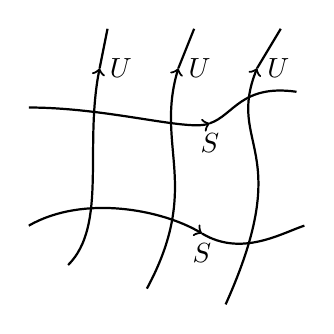
\begin{tikzpicture}
        \draw[thick, ->] (0,0) .. controls (0.5, 0.5) and (0.2,1.5) .. (0.4,2.5) node[right] {\(U\)};
        \draw[thick] (0.4,2.5) -- (0.5,3);
        \draw[thick, ->] (1,-0.3) .. controls (1.7, 1) and (1.1,1.5) .. (1.4,2.5) node[right] {\(U\)};
        \draw[thick] (1.4,2.5) -- (1.6,3);
        \draw[thick, ->] (2,-0.5) .. controls (2.9, 1.5) and (2,1.5) .. (2.4,2.5) node[right] {\(U\)};
        \draw[thick] (2.4,2.5) -- (2.7,3);

        \draw[thick, ->] (-0.5,2) .. controls (0.5, 2) and (1.5,1.7) .. (1.8,1.8) node[below] {\(S\)};
        \draw[thick] (1.8,1.8) .. controls (2.1,1.9) and (2.2,2.3) .. (2.9,2.2);
        \draw[thick, ->] (-0.5,0.5) .. controls (0.2, 0.9) and (1.2,0.7) .. (1.7,0.4) node[below] {\(S\)};
        \draw[thick] (1.7,0.4) .. controls (2.2,0.1) and (2.7,0.4) .. (3,0.5);
    \end{tikzpicture}
\end{wrapfigure}
Let \(\gamma(s,\lambda)\) take coordinates \(x^\mu(s,\lambda)\); we define the vector fields
\begin{equation}
    S^\mu = \pdv{x^\mu}{s} \qq{and} U^\mu = \pdv{x^\mu}{\lambda}.
\end{equation}
We also define the \emph{deviation vectors} (?) from the coordinates \(s,\lambda\) on the image of \(\gamma\),
\begin{equation}
    S = \pdv{s} \qq{and} U = \pdv{\lambda}.
\end{equation}

We have \([S,U] = 0\), so we can write \(U^b\nabla_bS^a = S^b\nabla_bU^a\), and thus obtain the \emph{geodesic deviation equation}
\begin{equation}
    U^c\nabla_c(U^b\nabla_bS^a)=R\indices{^a_b_c_d}U^bU^cS^d.
\end{equation}
A solution \(S^a\) to this equation along \(\gamma\) is called a \emph{Jacobi field}.

\subsection{Geodesic congruences}
\begin{defn}
    Let \(\mathcal{U}\in\mathcal{M}\) be open. A \emph{geodesic congruence} is a family of geodesics such that exactly one geodesic passes through each \(p\in\mathcal{U}\).
\end{defn}
Let \(U^a\) be the tangent vector of a geodesic congruence, normalised such that \(U^2 = -1\) if timelike, \(0\) if null, and \(1\) if spacelike. We define the \emph{velocity gradient} \(B\indices{^a_b} = \nabla_bU^a\). By the above we have \(U^b\nabla_bS^a = B\indices{^a_b}S^b\). It is easy to see that \(U_aB\indices{^a_b} = 0 = B\indices{^a_b}U^b\). We also have
\begin{equation}
    U\vdot\nabla(U\vdot S) = \underbrace{(U\vdot\nabla U^a)}_{=0}S_a + U^a U\vdot\nabla S_a = \underbrace{U^aB_{ab}}_{=0}S^b = 0,
\end{equation}
so \(U\vdot S\) is constant along any geodesic in the congruence.

Suppose we redefine our affine parameter \(\lambda \to \lambda' = \lambda - a(s)\). We have \(S'^a = S^a + \dv{a}{s}U^a\). \(S^a\) and \(S'^a\) point to the same geodesics, so we have a kind of gauge freedom here. Note that \(U\vdot S' = U\vdot S + \dv{a}{s}U^2\), so in the spacelike and timelike cases, we can choose \(a(s)\) such that \(U\vdot S=0\) at \(\lambda = 0\), and hence everywhere.

\subsection{Null geodesic congruences}
Things are less easy if \(U\) is null. Pick some spacelike hypersurface \(\Sigma\) that is tranverse to \(U\) (i.e.\ not tangent). Pick a vector field \(N^a\) such that \(N^2=0\) and \(N\vdot U = -1\) on \(\Sigma\), and additionally \(U\vdot\nabla N^a = 0\). It can be shown that this implies that \(N^2 = 0\) and \(N\vdot U=-1\) everywhere. Now write
\begin{equation}
    S^a = \alpha U^a + \beta N^a + \hat{S}^a
\end{equation}
where \(U\vdot \hat{S} = N\vdot\hat{S} = 0\) (this means that \(\hat{S}^a\) is either spacelike or zero). We have \(U\vdot S = -\beta\), so \(\beta\) is constant along each geodesic. Note that \(\alpha U^a + \hat{S}^a\) is orthogonal to \(U^a\) and \(\beta N^a\) is parallely transported along \(U^a\).

\begin{eg}
    Consider a null hypersurface \(\mathcal{N}\) and pick a congruence containing the generators of \(\mathcal{N}\). For a 1-parameter family of generators, we have \(S^a\) tangent to \(\mathcal{N}\), and so \(\beta = -U\vdot S = 0\).
\end{eg}

We can write \(\hat{S}^a = P\indices{^a_b}S^b\) where \(P\indices{^a_b} = \delta^a_b = N^aU_b + U^aN_b\). \(P\indices{^a_b}\) is a projection (\(P\indices{^a_b}P\indices{^b_c} = P\indices{^a_c}\)) onto \(T_\perp = \{\text{vectors \(\perp\) to \(U^a,N^a\)}\} \subset T_p(\mathcal{M})\), a 2d space.  We have \(U\vdot\nabla P\indices{^a_b} = 0\).

\begin{lemma}
    If \(U\vdot S = 0\), then \(U\vdot\nabla\hat{S}^a = \hat{B}\indices{^a_b}\hat{S}^b\), where \(\hat{B}\indices{^a_b} = P\indices{^a_c}B\indices{^c_d}P\indices{^d_b}\).
\end{lemma}
\begin{proof}
    We have:
    \begin{align}
        U\vdot\nabla\hat{S}^a &= U\vdot\nabla(P\indices{^a_c}S^c) \\
                              &= P\indices{^a_c}U\vdot\nabla S^c \\
                              &= P\indices{^a_c}B\indices{^c_d}S^d \\
                              &= P\indices{^a_c}B\indices{^c_d}P\indices{^d_e}S^e \quad \text{(using \(B\vdot U=U\vdot S=0\))} \\
                              &= \underbrace{P\indices{^a_c}B\indices{^c_d}P\indices{^d_b}}_{=\hat{B}\indices{^a_b}}\underbrace{P\indices{^b_e}S^e}_{=\hat{S}^b} \quad \text{(since \(P = P^2\))} \qedhere
    \end{align}
\end{proof}

\subsection{Expansion, rotation and shear}
\lecture{03/02/16}
\begin{defn}
    \emph{Expansion} \(\theta\), \emph{rotation} \(\hat{\omega}_{ab}\) and \emph{shear} \(\hat{\sigma}_{ab}\) are defined in the following way:
    \begin{equation}
        \theta = \hat{B}\indices{^a_a} \quad \hat{\omega} = \hat{B}_{[ab]} \quad \hat{\sigma}_{ab} = \hat{B}_{(ab)} - \frac{1}{2}P_{ab}\theta
    \end{equation}
\end{defn}
We have \(\hat{B}\indices{^a_b} = \frac{1}{2}\theta P\indices{^a_b} + \hat{\sigma}\indices{^a_b} + \hat{\omega}\indices{^a_b}\), and it can be shown that \(\theta = g^{ab}B_{ab} = \nabla_a U^a\).

\begin{lemma}
    If a congruence contains the generators of a null hypersurface \(\mathcal{N}\), then \(\hat{\omega}=0\) on \(\mathcal{N}\). Conversely, if \(\hat{\omega}=0\) then \(U^a\) is everywhere hypersurface orthogonal.
\end{lemma}
\begin{proof}
    Since \(B\vdot U = U\vdot B = 0\), we can write 
    \begin{equation}
        \hat{B}\indices{^b_c} = B\indices{^b_c} + U^bN_dB\indices{^d_c} + U_cB\indices{^b_d}N^d + U^bU_c N_dB\indices{^d_e}N^e.
    \end{equation}
    We have
    \begin{equation}
        U_{[a}\hat{\omega}_{bc]} = U_{[a}\hat{B}_{bc]} 
                                 = U_{[a}B_{bc]} 
                                 = U_{[a}\nabla_cU_{b]} 
                                 = - \frac{1}{6} (U\wedge\dd{U})_{abc},
    \end{equation}
    so since \(U^a\) is orthogonal to \(\mathcal{N}\) and hence \(U\wedge\dd{U} = 0\) on \(\mathcal{M}\), we can conclude
    \begin{equation}
        0 = \left. U_{[a}\hat{\omega}_{bc]} \right|_{\mathcal{N}} = \left.\frac{1}{3}(U_a\hat{\omega}_{bc} + U_b\hat{\omega}_{ca} + U_c\hat{\omega}_{ab}) \right|_{\mathcal{N}}.
    \end{equation}
    Contracting with \(N^a\), we see that \(\hat{\omega}_{bc} = 0\) on \(\mathcal{N}\) as required.

    For the converse, we have \(\hat{\omega} = 0 \implies U\wedge\dd{U}=0\), which by Frobenius' theorem implies \(U\) is hypersurface orthogonal.
\end{proof}

Consider geodesics in \(\mathcal{N}\) with tangent vector \(S^a\). By foliating \(\mathcal{N}\) into a family of constant \(\lambda\) surfaces, we can visualise how expansion and shear act on these geodesics.
\begin{figure}[H]
    \centering
    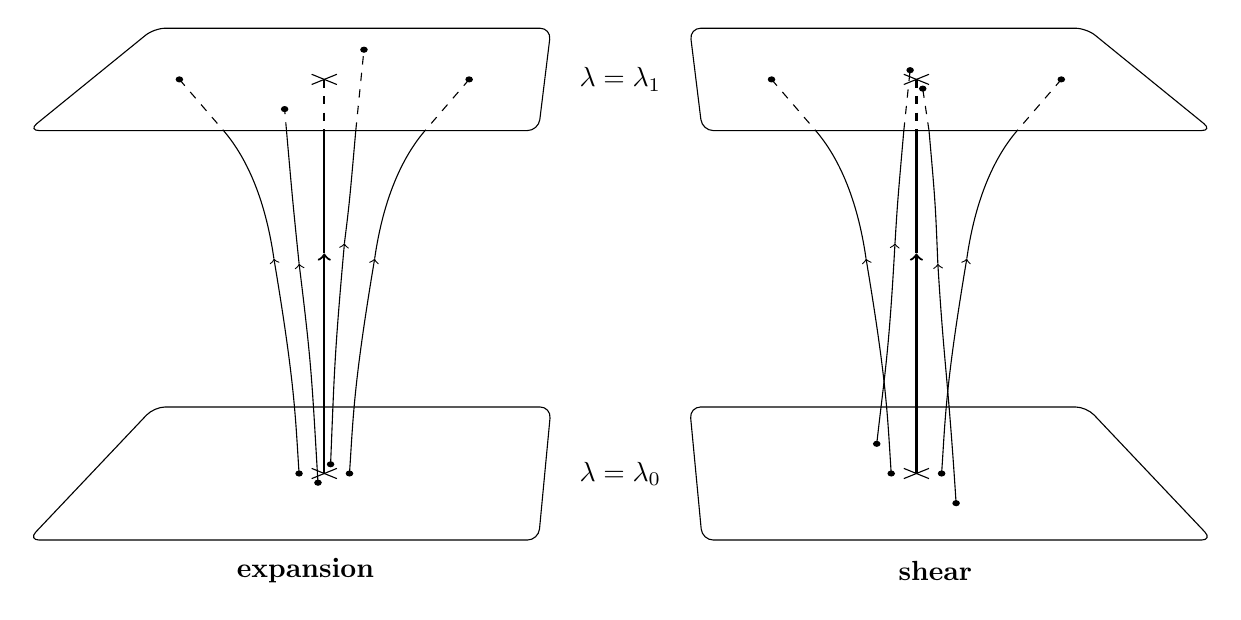
\begin{tikzpicture}[xscale=1.6,yscale=1.3]
        \begin{scope}[xscale=-1]
            \draw[rounded corners] (0.65,4) -- (4.7,4) -- (3.7,5) -- (0.55,5) -- cycle;
            \draw[rounded corners] (0.65,0) -- (4.7,0) -- (3.7,1.3) -- (0.55,1.3) -- cycle;

            \begin{scope}[shift={(4.7,0)},xscale=-1]
                \draw[->] (2.55,0.65) .. controls (2.58,1.2) and (2.58,1.5) .. (2.75,2.75);
                \draw (2.75,2.75) .. controls (2.82,3.35) and (2.975,3.75) .. (3.15,4);
                \draw[dashed] (3.5,4.5) -- (3.15,4);
                \fill (2.55,0.65) circle (0.03);
                \fill (3.5,4.5) circle (0.03);
            \end{scope}

            \draw[->] (2.55,0.65) .. controls (2.58,1.2) and (2.58,1.5) .. (2.75,2.75);
            \draw (2.75,2.75) .. controls (2.82,3.35) and (2.975,3.75) .. (3.15,4);
            \draw[dashed] (3.5,4.5) -- (3.15,4);
            \fill (2.55,0.65) circle (0.03);
            \fill (3.5,4.5) circle (0.03);

            \draw[->] (2.4,0.56) .. controls (2.45,1.6) and (2.45,1.7) .. (2.55,2.7);
            \draw (2.55,2.7) .. controls (2.6,3.3) .. (2.65, 4);
            \draw[dashed] (2.65,4) -- (2.665,4.21);
            \fill (2.4,0.56) circle (0.03);
            \fill (2.665,4.21) circle (0.03);

            \draw[->] (2.3,0.74) .. controls (2.27,1.65) and (2.27,1.8) .. (2.19,2.9);
            \draw (2.19,2.9) .. controls (2.15,3.3) .. (2.1, 4);
            \draw[dashed] (2.1,4) -- (2.035,4.79);
            \fill (2.3,0.74) circle (0.03);
            \fill (2.035,4.79) circle (0.03);

            \draw[thick,->] (2.35,0.65) -- (2.35,2.8);
            \draw[thick] (2.35,2.8) -- (2.35,4);
            \draw[thick,dashed] (2.35,4.5) -- (2.35,4);
            \begin{scope}[shift={(2.35,4.5)},yscale=0.5]
                \draw (-0.1,-0.1) -- (0.1,0.1);
                \draw (0.1,-0.1) -- (-0.1,0.1);
            \end{scope}
            \begin{scope}[shift={(2.35,0.65)},yscale=0.5]
                \draw (-0.1,-0.1) -- (0.1,0.1);
                \draw (0.1,-0.1) -- (-0.1,0.1);
            \end{scope}

            \node at (2.5,-0.3) {\bfseries expansion};
        \end{scope}
        \draw[rounded corners] (0.65,4) -- (4.7,4) -- (3.7,5) -- (0.55,5) -- cycle;
        \draw[rounded corners] (0.65,0) -- (4.7,0) -- (3.7,1.3) -- (0.55,1.3) -- cycle;

        \begin{scope}[shift={(4.7,0)},xscale=-1]
            \draw[->] (2.55,0.65) .. controls (2.58,1.2) and (2.58,1.5) .. (2.75,2.75);
            \draw (2.75,2.75) .. controls (2.82,3.35) and (2.975,3.75) .. (3.15,4);
            \draw[dashed] (3.5,4.5) -- (3.15,4);
            \fill (2.55,0.65) circle (0.03);
            \fill (3.5,4.5) circle (0.03);
        \end{scope}

        \draw[->] (2.55,0.65) .. controls (2.58,1.2) and (2.58,1.5) .. (2.75,2.75);
        \draw (2.75,2.75) .. controls (2.82,3.35) and (2.975,3.75) .. (3.15,4);
        \draw[dashed] (3.5,4.5) -- (3.15,4);
        \fill (2.55,0.65) circle (0.03);
        \fill (3.5,4.5) circle (0.03);

        \draw[->] (2.665,0.36) .. controls (2.6,1.6) and (2.57,1.7) .. (2.52,2.7);
        \draw (2.52,2.7) .. controls (2.5,3.3) .. (2.45, 4);
        \draw[dashed] (2.45,4) -- (2.4,4.41);
        \fill (2.665,0.36) circle (0.03);
        \fill (2.4,4.41) circle (0.03);

        \draw[->] (2.035,0.94) .. controls (2.1,1.65) and (2.13,1.8) .. (2.18,2.9);
        \draw (2.18,2.9) .. controls (2.2,3.3) .. (2.25, 4);
        \draw[dashed] (2.25,4) -- (2.3,4.59);
        \fill (2.035,0.94) circle (0.03);
        \fill (2.3,4.59) circle (0.03);

        \draw[thick,->] (2.35,0.65) -- (2.35,2.8);
        \draw[thick] (2.35,2.8) -- (2.35,4);
        \draw[thick,dashed] (2.35,4.5) -- (2.35,4);
        \begin{scope}[shift={(2.35,4.5)},yscale=0.5]
            \draw (-0.1,-0.1) -- (0.1,0.1);
            \draw (0.1,-0.1) -- (-0.1,0.1);
        \end{scope}
        \begin{scope}[shift={(2.35,0.65)},yscale=0.5]
            \draw (-0.1,-0.1) -- (0.1,0.1);
            \draw (0.1,-0.1) -- (-0.1,0.1);
        \end{scope}

        \node at (2.5,-0.3) {\bfseries shear};

        \node at (0,0.65) {\(\lambda=\lambda_0\)};
        \node at (0,4.5) {\(\lambda=\lambda_1\)};
    \end{tikzpicture}
\end{figure}
With expansion, geodesics move apart from one another for positive \(\theta\), and closer together for negative \(\theta\). If there is a shear, then geodesics move closer together in one direction, but further apart in the other.

\subsection{Gaussian null coordinates}
We can define a vector field \(V\) on \(\mathcal{N}\) by
\begin{equation}
    V^2 = 0, \quad V\vdot U = 1 \qq{and} V\vdot\pdv{y^i} = 0.
\end{equation}

\begin{wrapfigure}{r}{0.5\linewidth}
    \centering
    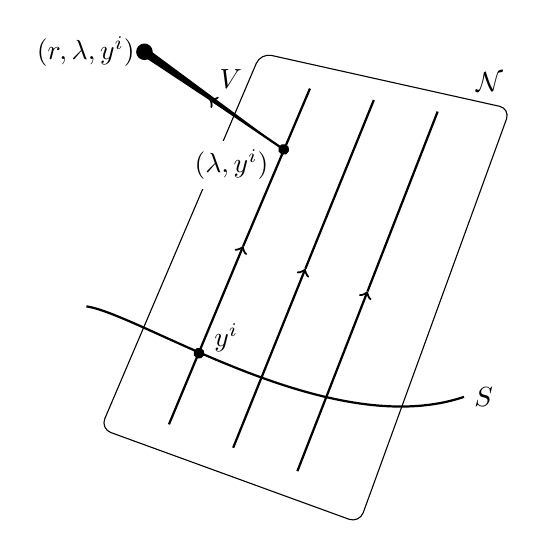
\begin{tikzpicture}[rotate=-20,scale=1.4]
        \node[above] at (2.3,4) {\(\mathcal{N}\)};
        \draw[rounded corners] (0,0) -- (2.5,0) -- (2.5,4) -- (0.2,3.7) -- cycle;
        \node[left, fill=white] at (0.695,2.8) {\((\lambda,y^i)\)};
        \draw[thick,->] (0.57,0.25) -- (0.65,2);
        \draw[thick] (0.65,2) -- (0.73,3.55);
        \draw[thick,->] (1.19,0.25) -- (1.25,2);
        \draw[thick] (1.25,2) -- (1.31,3.65);
        \draw[thick,->] (1.81,0.25) -- (1.85,2);
        \draw[thick] (1.85,2) -- (1.89,3.75);
        \draw[thick] (-0.5,1) .. controls (0,1.1) and (2,0.6) .. (3,1.4) node[right] {\(S\)};
        \fill (0.605,0.95) circle (0.05);
        \node[right] at (0.605,1.1) {\(y^i\)};
        \fill (0.695,2.95) circle (0.05);
        \draw[thick,->] (0.695,2.95) -- (-0.095,3.15) node[above right] {\(V\)};
        \fill (0.695,2.95) -- (-0.79,3.39) -- (-0.8,3.31) -- cycle;
        \fill (-0.795,3.35) circle (0.075) node[left] {\((r,\lambda,y^i)\)};
    \end{tikzpicture}
\end{wrapfigure}
To construct \emph{Gaussian null coordinates} near \(\mathcal{N}\), we assign the coordinates \((r,\lambda,y^i)\) to a point affine parameter distance \(r\) along a null geodesic starting at \((\lambda,y^i)\in\mathcal{N}\) with tangent \(V^a\) there.

Recall that \(U=\pdv{\lambda}\), so \(V=\pdv{r}\) is tangent to affinely parametrised null geodesics, so \(g_{rr} = 0\). Exercise: the geodesic equation reduces to \(g_{r\mu,r} = 0\). Therefore we have \(g_{r\lambda} = g_{r\lambda}|_{r=0} = U\vdot V|_{\mathcal{N}} = 1\) and \(g_{ri} = g_{ri}|_{r=0} = \left.V\vdot \pdv{y^i}\right|_{\mathcal{N}} = 0\). Also, since \(g_{\lambda\lambda}|_{r=0} = U^2|_{\mathcal{N}} = 0\) we have \(g_{\lambda\lambda} = rF\), and similarly since \(g_{\lambda i} |_{r=0} = \left. U\vdot\pdv{y^i}\right|_{\mathcal{N}} = 0\) we have \(g_{\lambda i} = r h_i\), where \(F\) and \(h_i\) are some smooth functions. Hence we have the following line element:
\begin{equation}
    \dd{s}^2 = 2\dd{r}\dd{\lambda} + rF\dd{\lambda}^2 + 2rh_i\dd{\lambda}\dd{y^i} + h_{ij}\dd{y^i}\dd{y^j}
\end{equation}
The induced line element on \(\mathcal{N}\) is therefore
\begin{equation}
    \dd{s}^2|_{\mathcal{N}} = 2\dd{r}\dd{\lambda} + h_{ij}\dd{y^i}\dd{y^j}.
\end{equation}
Using this metric, we can move the index downstairs on \(U^\mu|_{\mathcal{N}} = (0,1,0,0)\) to obtain \(U_\mu|_{\mathcal{N}} = (1,0,0,0)\), and hence from \(U\vdot B = B\vdot U = 0\), we have \(B\indices{^r_\mu} = B\indices{^\mu_\lambda} = 0\). Also
\begin{align}
    \theta = B\indices{^\mu_\mu} = B\indices{^i_i} &= \nabla_i U^i = \partial_i U^i + \Gamma^i_{i\mu}U^\mu \\
       &= \Gamma^i_{i\mu} = \frac{1}{2}(g_{\mu i,\lambda} + g_{\mu\lambda,i} - g_{i\lambda,\mu}) \\
       &= \frac{1}{2} h^{ij} (g_{ij,\lambda} + \underbrace{g_{j\lambda,i}}_{=0} - \underbrace{g_{i\lambda,j}}_{=0}) \\
       &= \frac{1}{2}h^{ij}\partial_\lambda h_{ij} = \frac{\partial_\lambda\sqrt{h}}{\sqrt{h}},
\end{align}
where \(h = \det h_{ij}\). Thus we have
\begin{equation}
    \pdv{\lambda}\sqrt{h} = \theta\sqrt{h}.
\end{equation}
\(\sqrt{h}\) is the area element on a surface of constant \(\lambda\) in \(\mathcal{N}\), so we can see why \(\theta\) is called the ``expansion''.

\subsection{Trapped surfaces}
Let \(\mathcal{S}\) be a 2d spacelike (orientable) surface. Given a point \(p \in \mathcal{S}\), there exist two independent future-directed null vectors orthogonal to \(\mathcal{S}\) at \(p\), say \(U_2, U_1\) (up to scaling). Thus there are two families of null geodesics starting on \(\mathcal{S}\) and orthogonal to \(\mathcal{S}\), and two null hypersurfaces \(\mathcal{N}_1\) and \(\mathcal{N}_2\) generated by these families. The two families are \emph{outgoing} and \emph{ingoing} light rays from \(S\). Let the expansion on these two surfaces be \(\theta_1\) and \(\theta_2\) respectively.

\begin{defn}
    A compact orientable spacelike 2-surface \(\mathcal{S}\) is \emph{trapped} if \(\theta_1, \theta_2 < 0\) everywhere on \(\mathcal{S}\). It is \emph{marginally trapped} if \(\theta_1, \theta_2 \le 0\) everywhere on \(\mathcal{S}\).
\end{defn}

\begin{eg}
    Consider \(\mathcal{S} = \{U=U_0,V=V_0\} \sim S^2\) in Kruskal spacetime. The generators of \(\mathcal{N}_i\) are the radial null geodesics with either \(U=\text{constant}\) or \(V=\text{constant}\).
    \begin{figure}[H]
        \centering
        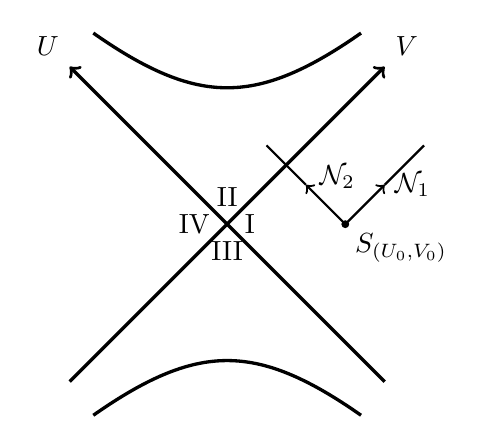
\begin{tikzpicture}
            \draw[domain=-1.7:1.7,smooth,variable=\x,very thick] plot({\x},{sqrt(3+\x*\x))});
            \draw[domain=-1.7:1.7,smooth,variable=\x,very thick] plot({\x},{-sqrt(3+\x*\x))});
            \draw[very thick,->] (-2,-2) -- (2,2) node[above right] {\(V\)};
            \draw[very thick,->] (2,-2) -- (-2,2) node[above left] {\(U\)};
            \draw (0.1,0) node[right] {I};
            \draw (0,0.1) node[above] {II};
            \draw (0,-0.1) node[below] {III};
            \draw (-0.1,0) node[left] {IV};
            
            \fill (1.5,0) circle (0.05) node[below right] {\(S_{(U_0,V_0)}\)};
            \draw[thick, ->] (1.5,0) -- (2,0.5) node[right] {\(\mathcal{N}_1\)};
            \draw[thick] (2,0.5) -- (2.5,1);
            \draw[thick, ->] (1.5,0) -- (1,0.5);
            \node[right] at (1.05,0.6) {\(\mathcal{N}_2\)};
            \draw[thick] (1,0.5) -- (0.5,1);
        \end{tikzpicture}
    \end{figure}
    Each null surface contains geodesic tangent vectors of the form \((\dd{U})^a\propto re^{\frac{r}{2M}}\left(\pdv{V}\right)^a = U_1^a\) and \((\dd{V})^a\propto re^{\frac{r}{2M}}\left(\pdv{U}\right)^a = U_2^a\) respectively. We have
    \begin{align}
        \theta_1 = \nabla_aU_1^a &= \frac{1}{\sqrt{-g}}\partial_\mu(\sqrt{-g}U_1^\mu) \\
                                 &= r^{-1}e^{\frac{r}{2M}}\partial_V(re^{-\frac{r}{2M}}re^{\frac{r}{2M}}) \\
                                 &= 2e^{\frac{r}{2M}} \partial_V r.
    \end{align}
    Using \(UV = -e^{\frac{r}{2M}}\left(\frac{r}{2M}-1\right)\) we can find \(\partial_V r\), and so can obtain \(\theta_1 = -\frac{8M^2}{r}U\). Similarly we have \(\theta_2 = -\frac{8M^2}{r}V\). We set \(U=U_0\) and \(V=V_0\) to find the expansion of the two surfaces.

    If \(\mathcal{S}\) is in region I, we have \(\theta_1>0\) and \(\theta_2<0\), so this is not a trapped surface. However, if \(\mathcal{S}\) is in the black hole region II, then \(\theta_1, \theta_2 < 0\), and so \(\mathcal{S}\) is trapped.
\end{eg}

\subsection{Raychaudhuri's equation}
\lecture{05/02/16}
\begin{lemma}
    \emph{Raychaudhuri's equation} holds:
    \begin{equation}
        \dv{\theta}{\lambda} = -\frac{1}{2}\theta^2 - \hat{\sigma}^{ab}\hat{\sigma}_{ab} + \hat{\omega}^{ab}\hat{\omega}_{ab} - R_{ab}U^aU^b
    \end{equation}
\end{lemma}
\begin{proof}
    We have 
    \begin{align}
        \dv{\theta}{\lambda} &= U\vdot\nabla(B\indices{^a_b}P\indices{^b_a}) = P\indices{^b_a}U\vdot\nabla B\indices{^a_b} \\
                             &= P\indices{^b_a}U^c\nabla_c\nabla_b U^a \\
                             &= P\indices{^b_a}U^c(\nabla_b\nabla_c U^a + R\indices{^a_{dcb}}U^d) \\
                             &= P\indices{^b_a}(\nabla_b(\underbrace{U^c\nabla_cU^a}_{=0}) - (\nabla_bU^c)\nabla_cU^a) + P\indices{^b_a} R\indices{^a_{dcb}}U^cU^d \\
                             &= - B\indices{^c_b}P\indices{^b_a}B\indices{^a_c} - R_{cd} U^cU^d \\
                             &= -\hat{B}\indices{^c_a}\hat{B}\indices{^a_c} - R_{ab}U^aU^b \\
                             &= -\frac{1}{2}\theta^2 - \hat{\sigma}^{ab}\hat{\sigma}_{ab} + \hat{\omega}^{ab}\hat{\omega}_{ab} - R_{ab}U^aU^b.
    \end{align}
\end{proof}

\subsection{Conditions on energy}
Often we will impose energy conditions on the energy momentum tensor.

\subsubsection*{Dominant energy condition}
This states that \(-T\indices{^a_b}V^b\) is a future-directed causal vector (or zero) for all future-directed timelike vectors \(V\). The DEC implies that if \(T_{ab} = 0\) in a closed \(\mathcal{S} \in \Sigma\), then \(T_{ab} = 0\) in \(D^+(\mathcal{S})\). Said another way: nothing can travel faster than the speed of light.

\begin{eg}
    Consider the energy-momentum tensor of a scalar field
    \begin{equation}
        T_{ab} = \partial_a\phi\partial_b\phi - \frac{1}{2}g_{ab}(\partial\phi)^2.
    \end{equation}
    We define \(j^a = -T\indices{^a_b}V^b\). We have
    \begin{equation}
        j^a = -(V\vdot\partial\phi)\partial^a\phi + \frac{1}{2}V^a(\partial\phi)^2 
        \implies
        j^2 = \frac{1}{4}\underbrace{V^2}_{<0}\underbrace{\left((\partial\phi)^2\right)^2}_{\ge 0} 
        \le 0,
    \end{equation}
    so \(j\) is causal or zero. Also
    \begin{equation}
        V\vdot j = -(V\vdot\partial\phi)^2 + \frac{1}{2}V^2(\partial\phi)^2 = \underbrace{-\frac{1}{2}(V\vdot\partial\phi)^2}_{\le 0} + \underbrace{\frac{1}{2}V^2}_{<0} \underbrace{\left[\partial\phi - \frac{V\vdot\partial\phi}{V^2}V\right]^2}_{\perp V^a \implies \ge 0} \le 0,
    \end{equation}
    so \(j\) is future-directed. Therefore scalar fields obey the DEC.
\end{eg}

\subsubsection*{Weak energy condition}
This states that \(T_{ab}V^aV^b\ge 0\) for all causal vectors \(V^a\). Note that DEC \(\implies\) WEC.

\subsubsection*{Null energy condition}
This states that \(T_{ab}V^aV^b\ge 0\) for all \emph{null} vectors \(V^a\). Note that WEC \(\implies\) NEC.

\subsubsection*{Strong energy condition}
This states that \((T_{ab}-\frac{1}{2}g_{ab}T\indices{^c_c})V^aV^b \ge 0\) for all causal vectors \(V^a\). Alternatively, using Einstein's equations, \(R_{ab}V^aV^b\ge0\), i.e.\ ``gravity is attractive''.

The SEC is independent to the other three; it is neither implied by, nor does it imply, any of the DEC, WEC or NEC.

\subsection{Conjugate points}
\begin{lemma}
    If both the Einstein equations and the NEC are obeyed, then the generators of a null hupersurface \(\mathcal{N}\) obey \(\dv{\theta}{\lambda}\le - \frac{1}{2}\theta^2\).
    \label{needed}
\end{lemma}
\begin{proof}
    We have \(\hat{\omega} = 0\) and \(\hat{\sigma}^{ab}\hat{\sigma}_{ab}\ge 0\), since vectors in \(T_\perp\) are spacelike. We also have by the NEC that \(R_{ab}U^aU^b = 8\pi T_{ab}U^aU^b \ge 0\) (using \(U^2 =0\)). Hence by Raychaudhuri's equation, we have \(\dv{\theta}{\lambda} \le \frac{1}{2}\theta^2\) as required.
\end{proof}
This has a simple corollary: \emph{if \(\theta = \theta_0\) at \(p \in \gamma\), where \(\gamma\) is a generator of \(\mathcal{N}\), then \(\theta \to -\infty\) within affine parameter \(\frac{2}{|\theta_0|}\), provided \(\gamma\) extends that far.}
\begin{proof}
    Without loss of generality, set \(\lambda = 0\) at \(p\). We have \(\dv{\lambda} \theta^{-1} \ge \frac{1}{2}\), so \(\theta^{-1}-\theta_0^{-1} \ge \frac{1}{2}\lambda\). Thus we have \(\theta \le \frac{\theta_0}{1+\lambda\theta_0/2}\), which approaches \(-\infty\) for some \(\lambda \le \frac{2}{|\theta_0|}\).
\end{proof}

\begin{defn}
    Two points \(p\) and \(q\) along a geodesic \(\gamma\) are said to be \emph{conjugate} if there exists a Jacobi field \(S^a\) along \(gamma\) such that \(S^a = 0\) at \(p,q\) but \(S^a \not\equiv 0\).
\end{defn}
Note that two points are conjugate iff the number of geodesics connecting them is more than one.

\begin{theorem}
    Consider a null conguence containing all null geodesics through \(p\). If \(\theta\to-\infty\) at \(q\) on a null geodesic \(\gamma\) through \(p\), then \(q\) is conjugate to \(p\) along \(\gamma\).
    \label{ineedthis}
\end{theorem}
\begin{theorem}
    Let \(\gamma\) be a causal curve containing points \(p,q\). Iff \(\gamma\) is a null geodesic with no point conjugate to \(p\) along \(\gamma\) between \(p\) and \(q\), then there does not exist a smooth 1-parameter family of causal curves \(\gamma_s\) connecting \(p,q\) such that \(\gamma_0=\gamma\) and \(\gamma_s\) is timelike for \(s>0\).
\end{theorem}

\begin{defn}
    Suppose we have a 2d spacelike surface \(\mathcal{S}\), with \(\mathcal{N}\) normal to \(S\) and \(\gamma\) a generator of \(\mathcal{N}\). We say that \(p\) is conjugate to \(\mathcal{S}\) along \(\gamma\) if there exists a Jacobi field \(S^a\) such that \(S^a=0\) at \(p\) and \(S^a|_{\mathcal{S}}\) is tangent to \(\mathcal{S}\).
\end{defn}

Note that \(p\) is conjugate to \(\mathcal{S}\) along \(\gamma\) iff \(\theta\to-\infty\) along \(\gamma\) in a congruence containing generators of \(\mathcal{N}\).

\subsection{Causal structure}
\begin{defn}
    Let \(\mathcal{U}\subset \mathcal{M}\), the \emph{chronological future} \(I^+(\mathcal{U})\) of \(\mathcal{U}\) is the set of all points \(q\) such that there exists a future-directed timelike curve from \(\mathcal{U}\) to \(q\). The \emph{causal future} \(J^+(\mathcal{U})\) is the set of all points \(q\) such that there exists a future-directed \emph{causal} curve from \(\mathcal{U}\) to \(q\). We define the chronological and causal pasts \(I^-(\mathcal{U})\) and \(J^-(\mathcal{U})\) similarly.
\end{defn}
\begin{eg}
    In Minkowski space, \(I^+(p)\) is the interior of the future lightcone of \(p\), and \(J^+(p)\) is the interior and surface of the future lightcone, including \(p\).
\end{eg}

\lecture{08/02/16}
We have that \(I^\pm(\mathcal{U})\) are open (since small deformations of timelike curves are also timelike). Recall that the \emph{closure} \(\overline{S}\) of a set \(S\) is the union of \(S\) with its limit points. In Minkowski space, we have \(\overline{I^\pm(p)} = J^\pm(p)\), but this is not true in general; for example, consider 2d Minkowski space with a point \(x\) deleted. If \(x\) is contained in the boundary of the future lightcone of \(p\), then \(\overline{I^\pm(p)} \ne J^\pm(p)\). Recall that the interior \(\operatorname{int}(S)\) of \(S\) is the set of all interior points of \(S\), i.e.\ those points \(q\) such that \(q\in V\subset S\) for some neighbourhood \(V\). The boundary \(\dot{S}\) of \(S\) is defined as \(\overline{S}\setminus\operatorname{int}(S)\).

\begin{theorem}
    Let \(p \in \mathcal{M}\). There exists a \emph{convex normal neighbourhood} of \(p\) (i.e.\ an open \(\mathcal{U}\in\mathcal{M}\) containing \(p\) such that for all \(q,r \in \mathcal{U}\) there is a unique geodesic from \(q\) to \(r\) that staus in \(\mathcal{U}\)). Furthermore, the chronological future of \(p\) in \(\mathcal{U}\) is the set of all points along future directed timelike geodesics in \(\mathcal{U}\) from \(p\), with boundary equal to the set of all points along future directed \emph{null} geodesics in \(\mathcal{U}\) from \(p\).
\end{theorem}
A corollary of this is: \emph{if \(q \in J^+(p)\setminus I^+(p)\), then there exists a null geodesic from \(p\) to \(q\)}.
\begin{lemma}
    If \(S\subset\mathcal{M}\), then (i) \(J^+(S)\subset\overline{I^+(S)}\), and (ii) \(I^+(S) = \operatorname{int}(J^+(S))\).
\end{lemma}
Note that \(I^+(S)\subset J^+(S)\), so (i) implies that \(\overline{I^+(S)} = \overline{J^+(S)}\), and (ii) implies that \(\dot{J}^+(S) = \dot{I}^+(S)\).
\begin{defn}
    \(S\subset \mathcal{M}\) is \emph{achronal} if no two points in \(S\) are connected by a timelike curve in \(\mathcal{M}\).
\end{defn}
\begin{theorem}
    Suppose \(\mathcal{U}\in\mathcal{M}\), then \(\dot{J}^+(\mathcal{U})\) is an achronal 3d submanifold of \(\mathcal{M}\).
    \label{achronalaf}
\end{theorem}
\begin{proof}[Proof of achronality]
    Assume \(p,q \in\dot{J}^+(\mathcal{U})\), with \(q\in I^+(p)\). 
    \begin{figure}[H]
        \centering
        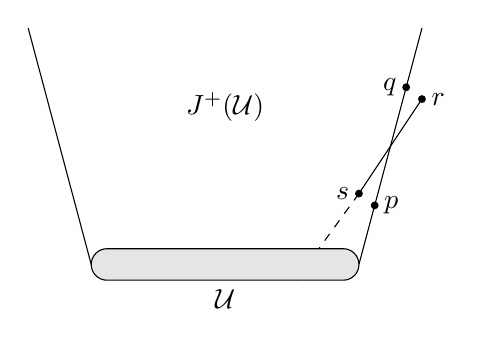
\begin{tikzpicture}
            \draw (0.8,0) -- (0,3);
            \draw (4.2,0) -- (5,3);
            \node at (2.5,2) {\(J^+(\mathcal{U})\)};

            \fill (4.4,0.75) circle (0.05) node[right] {\(p\)};
            \fill (4.8,2.25) circle (0.05) node[left] {\(q\)};

            \fill (4.2,0.9) circle (0.05) node[left] {\(s\)};
            \fill (5,2.1) circle (0.05) node[right] {\(r\)};

            \draw (4.2,0.9) -- (5,2.1);
            \draw[dashed] (4.2,0.9) -- (3.4,-0.2);

            \fill[gray!20] (1,0.2) arc (90:270:0.2) -- (4,-0.2) arc (270:450:0.2) -- cycle;
            \draw (1,0.2) arc (90:270:0.2) -- (4,-0.2) arc (270:450:0.2) -- cycle;
            \node[below] at (2.5,-0.2) {\(\mathcal{U}\)};
        \end{tikzpicture}
    \end{figure}
    Since \(I^+(p)\) is open, there exists a point \(r\) near \(q\) such that \(r \in I^+(p)\) and \(r \in J^+(\mathcal{U})\). Similarly, since \(I^-(r)\) is open, there exists a point \(s\) near \(p\) such that \(s \in I^-(r)\) and \(s \in J^+(\mathcal{U})\). But then we have a causal curve from \(\mathcal{U}\) to \(s\) to \(r\) that leaves \(J^+(\mathcal{U})\), which is a contradiction.
\end{proof}
\begin{theorem}
    Suppose \(\mathcal{U}\in\mathcal{M}\) is closed and suppose \(r \in \dot{J}^+(\mathcal{U})\) and \(r \not\in \mathcal{U}\). Then \(r\) lies on a null geodesic \(\lambda\), where \(\lambda\) lies entirely in \(\dot{J}^+(\mathcal{U})\) and is either past-inextendable or has a past endpoint on \(\mathcal{U}\).
\end{theorem}
\begin{theorem}
    Let \(\mathcal{S}\) be a 2d spacelike orientable compact submanifold of a globally hyperbolic spacetime. Then every \(p \in \dot{J}^+(\mathcal{S})\) lies on a future-directed null geodesic starting on and orthogonal to \(\mathcal{S}\), with no point conjugate to \(\mathcal{S}\) between \(\mathcal{S}\) and \(p\).
    \label{alsoneeded}
\end{theorem}
\begin{defn}
    The \emph{future Cauchy horizon} of a partial caucy surface \(H^+(\Sigma)=\overline{D^+(\Sigma)}\setminus I^-(D^+(\Sigma))\). \(H^-(\Sigma)\) is defined similarly.
\end{defn}
Note that \(H^\pm(\Sigma)\) are null hypersurfaces.

\begin{theorem}[Penrose singularity theorem, 1965]
    We assume the following:
    \begin{itemize}
        \item \((\mathcal{M},g)\) is a globally hyperbolic spacetime with non-compact Cauchy surface \(\Sigma\).
        \item \((\mathcal{M},g)\) satisfies the Einstein equations and the NEC.
        \item \(\mathcal{M}\) contains a trapped surface \(T\).
    \end{itemize}
    Let \(\theta_0 = \max_T\theta\) where we take the maximum over both sets of null geodesics orthogonal to \(T\) (note \(\theta_0 < 0\)).
    
    Then we have: at least one null geodesic orthogonal to \(T\) is future inextendable and has affine length less than or equal to \(\frac{2}{|\theta_0|}\).
\end{theorem}
\begin{proof}
    Suppose all future-inextendable null geodesics orthogonal to \(T\) have affine length greater than \(\frac{2}{|\theta_0|}\). By the corollary to Lemma~\ref{needed}, \(\theta \to -\infty\) along all such geodesics. By Theorem~\ref{ineedthis}, on each geodesic there is a point \(q\) that is conjugate to \(T\) that is affine parameter distance \(\lambda \le \frac{2}{\theta_0}\) from \(T\).

    Now let \(p \in \dot{J}^+(T)\), \(p \not\in T\). Since trapped surfaces are by definition 2d, spacelike, orientable and compact, we can apply Theorem~\ref{alsoneeded} to deduce that \(p\) lies on a future-directed null geodesic starting on and orthogonal to \(T\) with not point conjugate to \(T\) between \(T\) and \(p\). Hence, using the above, \(p\) must be affine parameter less than or equal to \(\frac{2}{|\theta_0|}\) from \(T\). So we have
    \begin{equation}
        \dot{J}^+(T) \subset \left\{\text{points along geodesics \(\perp\) to \(T\) with affine parameter distance \(\le \frac{2}{\theta_0}\)}\right\}.
    \end{equation}
    Note that the former set is closed while the latter is compact, so we can deduce that \(\dot{J}^+(T)\) is compact. Let \(\alpha:\dot{J}^+(T)\to\Sigma\) be a function that carries back a point \(p \in \dot{J}^+(T)\) along the orbits of some timelike vector field onto \(\Sigma\) (since \(\Sigma\) is a Cauchy surface, \(\alpha\) is well-defined). Since \(\dot{J}^+(T)\) is achronal (Theorem~\ref{achronalaf}), \(\alpha\) is a one to one map. Also, \(\alpha\) is continuous and is thus a homeomorphism. Since \(\dot{J}^+(T)\) is closed, so then is \(\alpha(\dot{J}^+(T))\). Also, since \(\dot{J}^+(T)\) is a manifold, \(\alpha(\dot{J}^+(T))\) must also be open. Since \(\mathcal{M}\) is connected, so too is \(\Sigma\), and hence we must have \(\alpha(\dot{J}^+(T)) = \Sigma\). But \(\Sigma\) is non-compact, while \(\dot{J}^+(T)\) is compact, so this is a contradiction.
\end{proof}

\section{Asymptotic Flatness}
\lecture{10/02/16}
\subsection{Conformal compactification}
\begin{defn}
    Given a spacetime \((\mathcal{M},g)\), a conformal transformation modifies the metric \(g \to \overline{g} = \Omega^2 g\), where \(\Omega:\mathcal{M}\to\RR\) is greater than 0.
\end{defn}

To \emph{conformally compactify} a spacetime, we will want \(\Omega \to 0\) ``at infinity''. More precisely, we choose \(\Omega\) such that \((\mathcal{M},\overline{g})\) is extendable onto \((\overline{\mathcal{M}}, \overline{g})\), a so-called \emph{unphysical} spacetime, and on the boundary of \(\mathcal{M}\) in \(\overline{\mathcal{M}}\) (``infinity'' in \(\mathcal{M}\)), we require \(\Omega=0\).
\begin{figure}[H]
    \centering
    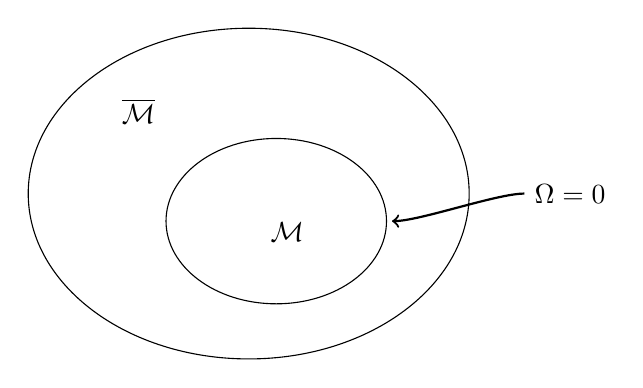
\begin{tikzpicture}[scale=0.7]
        \draw (0,0) ellipse (4 and 3);
        \draw (0.5,-0.5) ellipse (2 and 1.5);
        \node at (0.7,-0.7) {\(\mathcal{M}\)};
        \node at (-2,1.5) {\(\overline{\mathcal{M}}\)};

        \draw[thick,<-] (2.6,-0.5) .. controls (3.1,-0.5) and (4.5,0) .. (5,0) node[right] {\(\Omega = 0\)};
    \end{tikzpicture}
\end{figure}

For example, consider 3+1 Minkowski space, with the metric \(\dd{s}^2 = -\dd{t}^2 + \dd{r}^2 + r^2\dd{\omega}^2\), where \(\dd{\omega}^2\) is the round metric on the unit 2-sphere. Reparametrise into retarded time \(u = t-r\) and advanced time \(v = t+r\), to obtain \(\dd{s}^2 = -\dd{u}\dd{v} + \frac{1}{4}(u-v)^2\dd{\omega}^2\). Note that since \(r\ge0\), we have \(-\infty < u \le v < \infty\). If we define new coordinates \(p\) and \(q\) by \(u=\tan p\) and \(v=\tan q\), we see that we obtain a finite range \(-\frac{\pi}{2} < p \le q < \frac{\pi}{2}\) and \(\dd{s}^2 = (2\cos p\cos q)^{-2}\left[-4\dd{p}\dd{q}+\sin^2(q-p)\dd{\omega}^2\right]\). We see that we can carry out a conformal transformation with \(\Omega = 2\cos p\cos q\) to obtain an unphysical metric \(\overline{\dd{s}}^2 = -4\dd{p}\dd{q}+\sin^2(q-p)\dd{\omega}^2\). Finally, we reparametrise with \(T=q+p\) and \(\chi=q-p\) and get 
\begin{equation}
    \overline{\dd{s}}^2 = -\dd{T}^2 + \dd{\chi}^2 + \sin^2\chi\dd{\omega}^2.
\end{equation}
\(\dd{\chi}^2 + \sin^2\chi\dd{\omega}^2\) is the round metric of the unit 3-sphere, and we see that we obtain just the Einstein static universe, except for one crucial difference. In the ESU, \(T\in(-\infty,\infty)\) and \(\chi\in[0,\pi)\), but here we have \(T\in(-\pi,\pi)\) and \(\chi\in[0,\pi)\). Thus we choose \((\overline{\mathcal{M}},\overline{g}) = \text{ESU}\) as an extension of \((\mathcal{M},\overline{g})\), and identify ``infinity'' of \((\mathcal{M},g)\) as the points \(i^\pm\), \(i^0\) and the null hypersurfaces \(\scri^\pm\) given by \(T=\pm(\pi-\chi)\):
\begin{figure}[H]
    \centering
    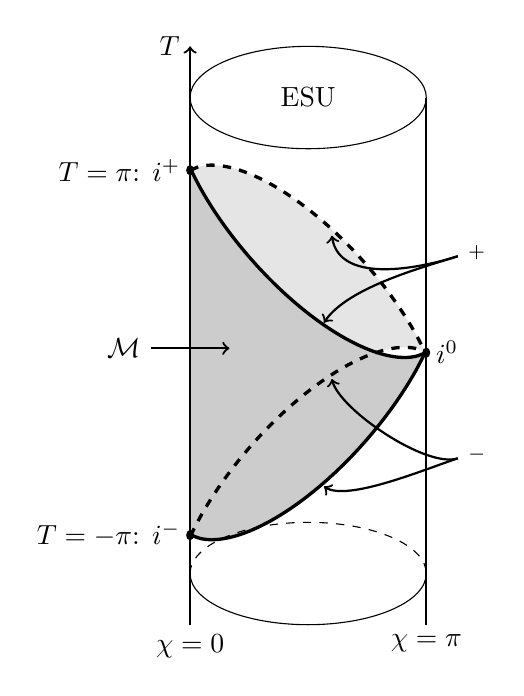
\begin{tikzpicture}[yscale=1.3]
        \begin{scope}
            \fill[domain=-1.495:1.495,smooth,variable=\x,dashed,very thick,gray!20] plot({\x+1.5},{3.02+0.6*(sqrt(3-\x*\x)-\x)}) -- (0.005,0.875);
            \fill[domain=-1.495:1.495,smooth,variable=\x,dashed,very thick,white] plot({\x+1.5},{1.24+0.6*(sqrt(3-\x*\x)+\x)});
        \end{scope}
        \begin{scope}
            \fill[domain=-1.495:1.495,smooth,variable=\x,very thick,gray!40] plot({\x+1.5},{2.3+0.6*(-sqrt(3-\x*\x)+\x)});
            \fill[domain=-1.495:1.495,smooth,variable=\x,very thick,gray!40] (0.005,0.875) -- plot({\x+1.5},{4.08+0.6*(-sqrt(3-\x*\x)-\x)});
        \end{scope}
        \draw[thick,->] (0,0) node[below] {\(\chi=0\)} -- (0,5.65) node[left] {\(T\)};
        \draw (1.5,5.15) ellipse (1.5 and 0.5);
        \draw[thick] (3,5.15) -- (3,0) node[below] {\(\chi=\pi\)};
        \draw[shift={(0,0.5)},yscale={1/3},dashed] (0,0) arc (180:0:1.5);
        \draw[shift={(0,0.5)},yscale={1/3}] (0,0) arc (180:360:1.5);
        \draw[domain=-1.495:1.495,smooth,variable=\x,very thick] plot({\x+1.5},{2.3+0.6*(-sqrt(3-\x*\x)+\x)});
        \draw[domain=-1.495:1.495,smooth,variable=\x,dashed,very thick] plot({\x+1.5},{1.24+0.6*(sqrt(3-\x*\x)+\x)});
        \draw[domain=-1.495:1.495,smooth,variable=\x,very thick] plot({\x+1.5},{4.08+0.6*(-sqrt(3-\x*\x)-\x)});
        \draw[domain=-1.495:1.495,smooth,variable=\x,dashed,very thick] plot({\x+1.5},{3.02+0.6*(sqrt(3-\x*\x)-\x)});

        \fill (0,0.875) circle (0.05) node[left] {\(T=-\pi\): \(i^-\)};
        \fill (0,4.44) circle (0.05) node[left] {\(T=\pi\): \(i^+\)};
        \fill (3,2.6575) circle (0.05) node[right] {\(i^0\)};
        \draw[thick,<-] (1.7,2.95) .. controls (2,3.3) and (3,3.5) .. (3.4,3.6) node[right] {\(\scri^+\)};
        \draw[thick,<-] (1.8,3.8) .. controls (1.9,3.3) and (3,3.5) .. (3.4,3.6);

        \draw[thick,<-] (1.7,1.35) .. controls (2,1.2) and (3,1.525) .. (3.4,1.625) node[right] {\(\scri^-\)};
        \draw[thick,<-] (1.8,2.4) .. controls (1.9,2.1) and (3,1.525) .. (3.4,1.625);
        \node at (1.5,5.15) {ESU};
        \draw[thick,<-] (0.5,2.7) -- (-0.5,2.7) node[left] {\(\mathcal{M}\)};
    \end{tikzpicture}
\end{figure}
If we denote each \(S^2\) at a given \(T\) and \(\chi\) by a single point, we obtain the so-called \emph{Penrose diagram} for Minkowski space:
\begin{figure}[H]
    \centering
    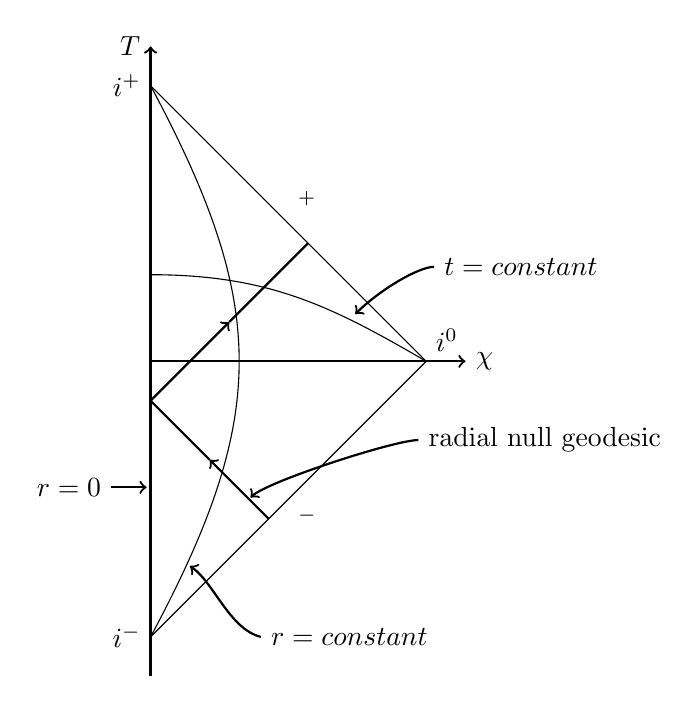
\begin{tikzpicture}
        \draw[thick,->] (0,-4) -- (0,4) node[left] {\(T\)};
        \draw[thick,->] (0,0) -- (4,0) node[right] {\(\chi\)};

        \draw (0,-3.5) -- (3.5,0) -- (0,3.5);
        
        \draw[thick,->] (1.5,-2) -- (0.75,-1.25);
        \draw[thick,->] (0.75,-1.25) -- (0,-0.5) -- (1,0.5);
        \draw[thick] (1,0.5) -- (2,1.5);

        \draw (0,-3.5) .. controls (1.5,-0.7) and (1.5,0.7) .. (0,3.5);
        \draw (0,1.1) .. controls (1.5,1.1) and (2.3,0.7) .. (3.5,0);

        \node[left] at (0,-3.5) {\(i^-\)};
        \node[left] at (0,3.5) {\(i^+\)};
        \node[above right] at (3.5,0) {\(i^0\)};

        \node[below right] at (1.75,-1.75) {\(\scri^-\)};
        \node[above right] at (1.75,1.75) {\(\scri^+\)};

        \draw[thick,<-] (0.5,-2.6) .. controls (0.8,-2.8) and (1,-3.4) .. (1.4,-3.5) node[right] {\(r = \text{constant}\)};
        \draw[thick,<-] (2.6,0.6) .. controls (2.9,0.9) and (3.4,1.2) .. (3.6,1.2) node[right] {\(t = \text{constant}\)};
        \draw[thick,<-] (1.27,-1.73) .. controls (1.47,-1.53) and (3.1,-1) .. (3.4,-1) node[right] {radial null geodesic};

        \draw[thick,<-] (-0.05,-1.6) -- (-0.5,-1.6) node[left] {\(r=0\)};
    \end{tikzpicture}
\end{figure}
This is a bounded subset of \(\RR^2\) with the flat metric. The boundary is the union of infinity with the axis (\(r=0\)). The different components of infinity have different names: \(\scri^-\) and \(\scri^+\) are \emph{past} and \emph{future null infinity} respectively, \(i^-\) and \(i^+\) are \emph{past} and \emph{future timelike infinity} respectively, and \(i^0\) is spatial infinity.

Suppose we have a massless scalar field obeying \(\nabla_a\nabla^a\psi=0\). Exercise: show that the general spherically symmetric solution is
\begin{equation}
    \psi(t,r) = \frac{1}{r}\left(f(u)+g(v)\right) = \frac{1}{r}\left(f(t-r)+g(t+r)\right).
\end{equation}
We need this to be smooth at \(r=0\) so we set \(g(x) = -f(x)\). Thus \(\psi(t,r) = \frac{1}{r}\left(f(u)-f(v)\right) = \frac{1}{r}\left(F(p)-F(q)\right)\), where \(F(x) = f(\tan x)\). Now let \(F_0(q) = (r\psi)_{\scri^-}\). Since \(p=-\frac{\pi}{2}\) on \(\scri^-\), we have \(F_0(q) = F(-\pi/2) - F(q)\). Therefore,
\begin{equation}
    \psi(t,r) = \frac{1}{r}\left(F_0(q)-F_0(p)\right),
\end{equation}
so the solution is uniquely determined everywhere by its behaviour on \(\scri^-\).

Suppose we had instead considered 2D Minkowski space, \(\dd{s}^2 = -\dd{t}^2 + \dd{r}^2\). Now the range of \(r\) is \((-\infty,\infty)\). Proceeding as before, we have \(-\infty < u,v < \infty\) and so \(-\frac{\pi}{2}<p,q<\frac{\pi}{2}\). Thus \(T,\chi\in(-\pi,\pi)\), and the Penrose diagram is now a square.
\begin{figure}[H]
    \centering
    \begin{tikzpicture}
        \draw (3,0) -- (0,3) -- (-3,0) -- (0,-3) -- cycle;

        \node[right] at (3,0) {\(i^0_R\)};
        \node[above] at (0,3) {\(i^+\)};
        \node[left] at (-3,0) {\(i^0_L\)};
        \node[below] at (0,-3) {\(i^-\)};

        \node[above right] at (1.5,1.5) {\(\scri^+_R\)};
        \node[above left] at (-1.5,1.5) {\(\scri^+_L\)};
        \node[below left] at (-1.5,-1.5) {\(\scri^-_L\)};
        \node[below right] at (1.5,-1.5) {\(\scri^-_R\)};

        \draw[thick,->] (2,-1) -- (0,1);
        \draw[thick] (0,1) -- (-1,2);
        \draw[thick,->] (-1,-2) -- (0.5,-0.5);
        \draw[thick] (0.5,-0.5) -- (2,1);
    \end{tikzpicture}
\end{figure}

We can carry out a similar procedure in the Kruskal spacetime. We define \(P=P(U)\) and \(Q=Q(V)\) such that \(P,Q\in\left(-\frac{\pi}{2},\frac{\pi}{2}\right)\), and we find a conformal factor \(\Omega\) such that \(\overline{g}\) extends onto \(\overline{\mathcal{M}}\), and \(\mathcal{M}\in\overline{\mathcal{M}}\) has boundary at \(P = \pm\frac{\pi}{2}\) or \(Q=\pm\frac{\pi}{2}\). We find that null infinity has four components: \(\scri^\pm\) in region I, and \({\scri^\pm}'\) in region IV.

\begin{figure}[H]
    \centering
    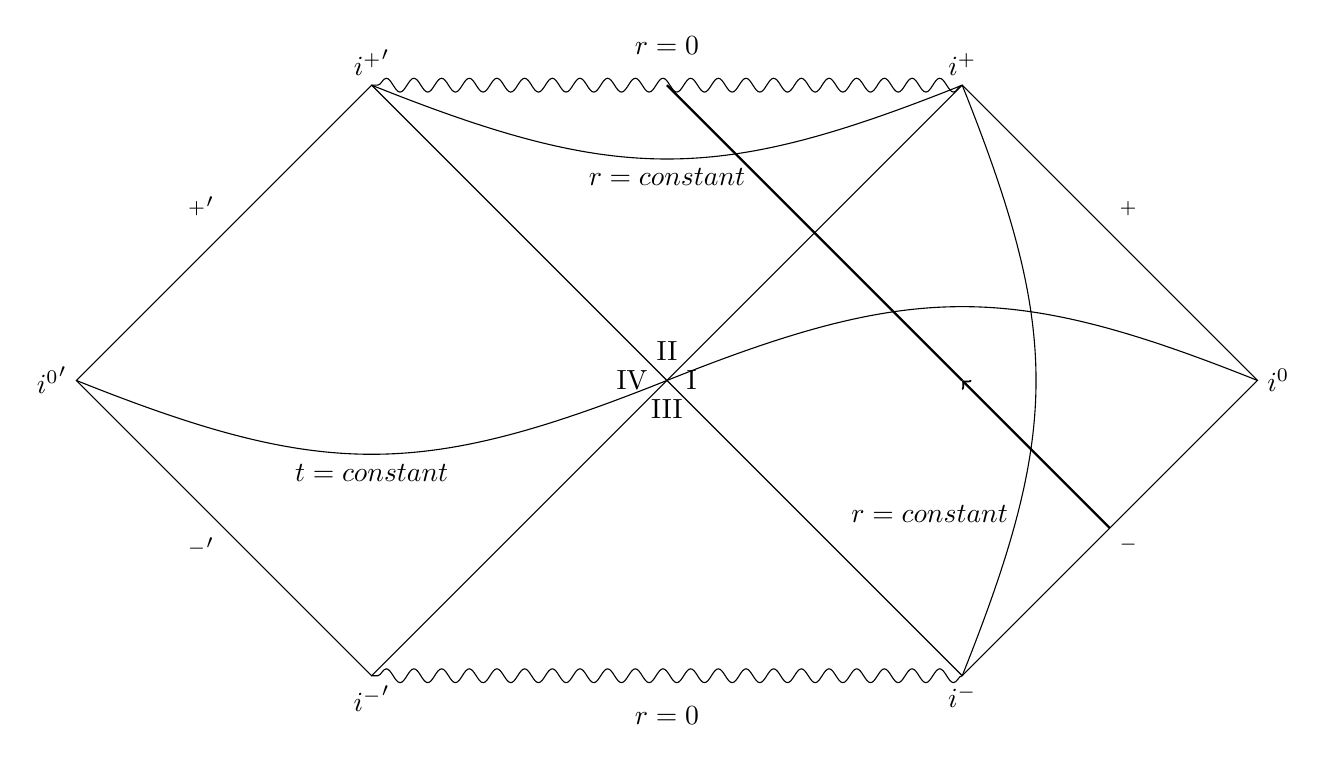
\begin{tikzpicture}[scale=1.25]
        \draw (3,3) -- (6,0) -- (3,-3) -- (-3,3) -- (-6,0) -- (-3,-3) -- cycle;
        \draw[decorate,decoration=snake] (3,3) -- (-3,3);
        \draw[decorate,decoration=snake] (3,-3) -- (-3,-3);

        \draw (0.1,0) node[right] {I};
        \draw (0,0.1) node[above] {II};
        \draw (0,-0.1) node[below] {III};
        \draw (-0.1,0) node[left] {IV};

        \node[right] at (6,0) {\(i^0\)};
        \node[above] at (3,3) {\(i^+\)};
        \node[above] at (-3,3) {\({i^+}'\)};
        \node[left] at (-6,0) {\({i^0}'\)};
        \node[below] at (3,-3) {\(i^-\)};
        \node[below] at (-3,-3) {\({i^-}'\)};

        \node[above right] at (4.5,1.5) {\(\scri^+\)};
        \node[above left] at (-4.5,1.5) {\({\scri^+}'\)};
        \node[below left] at (-4.5,-1.5) {\({\scri^-}'\)};
        \node[below right] at (4.5,-1.5) {\(\scri^-\)};

        \draw (6,0) .. controls (3.5,1) and (2.5,1) .. (0,0);
        \draw (-6,0) .. controls (-3.5,-1) and (-2.5,-1) .. (0,0) 
            node[midway,below] {\(t=\text{constant}\)};

        \draw (3,3) .. controls (4,0.5) and (4,-0.5) .. (3,-3)
            node [near end, left] {\(r=\text{constant}\)};
        \draw (-3,3) .. controls (-0.5,2) and (0.5,2) .. (3,3)
            node [midway,below] {\(r=\text{constant}\)};
        
        \draw[thick,->] (4.5,-1.5) -- (3,0);
        \draw[thick] (3,0) -- (0,3);

        \node at (0,3.4) {\(r=0\)};
        \node at (0,-3.4) {\(r=0\)};
    \end{tikzpicture}
\end{figure}

We can also draw a Penrose diagram for gravitational collapse:
\begin{figure}[H]
    \centering
    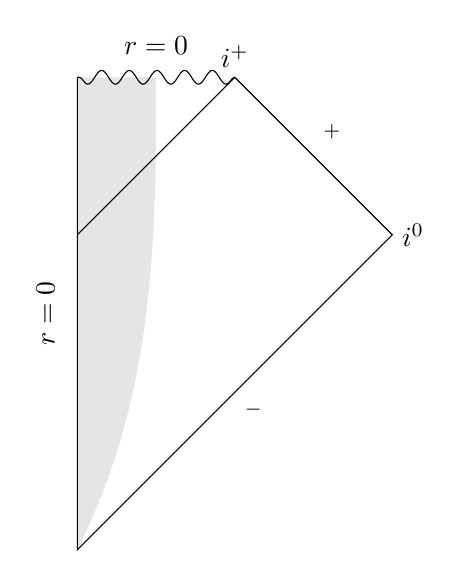
\begin{tikzpicture}[]
        \fill[gray!20] (0,6) -- (0,0) .. controls (1,2) and (1,4) .. (1,6) -- cycle;
        \draw (0,6) -- (0,0) -- (4,4) -- (2,6) -- (0,4);
        \draw[decorate,decoration=snake] (2,6) -- (0,6);
        
        \node at (1,6.4) {\(r=0\)};
        \node[rotate=90] at (-0.4,3) {\(r=0\)};
        
        \node[right] at (4,4) {\(i^0\)};
        \node[above] at (2,6) {\(i^+\)};

        \node[above right] at (3,5) {\(\scri^+\)};
        \node[below right] at (2,2) {\(\scri^-\)};
    \end{tikzpicture}
\end{figure}

\lecture{12/02/16}
\subsection{Asymptotic flatness}

\begin{defn}
    A time orientable spacetime \((\mathcal{M},g)\) is \emph{asymptotically flat} at null infinity if there exists a \((\overline{\mathcal{M}},\overline{g})\) such that:
    \begin{enumerate}
        \item There exists a positive \(\Omega:\mathcal{M}\to\RR\) such that \((\overline{\mathcal{M}},\overline{g})\) is an extension of \((\mathcal{M},\Omega^2g)\) (where we regard \(\mathcal{M}\) as a subset of \(\overline{\mathcal{M}}\) on which \(\overline{g}=\Omega^2g\)).
        \item We can extend \(\mathcal{M}\) within \(\overline{\mathcal{M}}\) to obtain a manifold with boundary \(\mathcal{M}\cup\partial\mathcal{M}\) (a \emph{manifold with boundary} is just like a manifold, but charts are \(\mathcal{M}\to\RR/2=\{(x^1,\dots,x^n):x^n\le0\}\)).
        \item \(\Omega\) smoothly extends to \(\overline{\mathcal{M}}\) such that \(\left.\Omega\right|_{\partial\mathcal{M}}=0\) and \(\left.\dd{\Omega}\right|_{\partial\mathcal{M}}\ne0\).
        \item We can choose \(\scri^\pm\) such that \(\partial\mathcal{M} = \scri^+\cup\scri^-\), \(\scri^+\cap\scri^- = \varnothing\), and \(\scri^\pm \simeq \RR\times S^2\).
        \item No future or past directed causal curves in \(\mathcal{M}\) intersect \(\scri^-\) or \(\scri^+\) respectively.
        \item \(\scri^\pm\) are ``complete'' (to be defined shortly).
    \end{enumerate}
\end{defn}

\begin{eg}
    Consider the Schwarzschild solution in outgoing Eddington-Finklestein coordinates:
    \begin{equation}
        g = -\left(1-\frac{2M}{r}\right)\dd{u}^2 - 2\dd{u}\dd{r}+r^2\dd{\omega}^2
    \end{equation}
    Setting \(r=\frac{1}{x}\) and carrying out a conformal transformation with \(\Omega = x\), we obtain
    \begin{equation}
        \overline{g} = -x^2(1-2Mx)\dd{u}^2 + 2\dd{u}\dd{x} + \dd{\omega}^2.
    \end{equation}
    We can extend \(\overline{g}\) smoothly across \(\scri^+=\{x=0\}\). \(\scri^+\) is parametrised by \((u,\theta,\phi)\), so \(\scri^+ \simeq \RR\times S^2\).
\end{eg}

It can be shown that under a conformal transformation, the Ricci tensor transforms as 
\begin{equation}
    R_{ab}=\overline{R}_{ab} + 2\Omega^{-1}\overline{\nabla}_a\overline{\nabla}_b\Omega + \overline{g}_{ab}\overline{g}^{cd}\left(\Omega^{-1}\overline{\nabla}_c\overline{\nabla}_d\Omega - 3\Omega^{-2}\partial_c\Omega\partial_d\Omega\right).
\end{equation}
Multiplying by \(\Omega\) gives
\begin{equation}
    \Omega R_{ab} = \underbrace{\Omega\overline{R}_{ab} + 2\overline{\nabla}_a\overline{\nabla}_b\Omega + \overline{g}_{ab}\overline{g}^{cd}\overline{\nabla}_c\overline{\nabla}_d\Omega}_{\text{A}} - \underbrace{3\Omega^{-1}\overline{g}_{ab}\overline{g}^{cd}\partial_c\Omega\partial_d\Omega}_{\text{B}}.
\end{equation}
We assume that \(\Omega R_{ab}\) is 0 at \(\scri^+\) (as would be the case for a sufficiently quickly reached vacuum at infinity) and observe that since A is smooth at \(\scri^+\), then so must B be. Since \(\Omega^{-1}\) diverges at \(\scri^+\), we must thus have \(\left.\overline{g}^{cd}\partial_c\Omega\partial_d\Omega\right|_{\scri^+}=0\). Hence \(\left.\dd{\Omega}\right|_{\scri^+}\) is null. Since \(\scri^+\) is a surface of constant \(\Omega\), we then have that \(\scri^+\) is a null hypersurface in \((\overline{\mathcal{M}},\overline{g})\).

Note that we have some gauge freedom in our choice of conformal factor. We could just as well have chosen \(\Omega'=\omega\Omega\), where \(\omega:\overline{\mathcal{M}}\to\RR\) is some positive function on \(\mathcal{M}\cup\partial\mathcal{M}\). It is possible to choose a gauge such that \(\left.\overline{\nabla}_a\overline{\nabla}_b\Omega\right|_{\scri^+} = 0\) (\(\dagger\)). Assume that we take this gauge and define \(n^a = g^{ab}(\dd{\Omega})_b\). We have \(\left.\overline{\nabla}_an^b\right|_{\scri^+}=0\), so \(B\indices{^b_a}\) -- the expansion and shear of the generators of \(\scri^+\) are zero.

We can define a natural set of coordinates in the neighbourhood of \(\scri^+\) in the following way. Firstly we have spherical coordinates \((\theta,\phi)\) on the spheres at each point of \(\scri^+\), with metric \(\left.\overline{g}_{ab}\right|_{S^2} = \dd{\theta}^2+\sin^2\theta\dd{\phi}^2\). \(n^a\) is tangent to \(\scri^+\), so we can use the distance \(u\) along its integral curves as a third coordinate on \(\scri^+\). Now there is a unique null direction perpendicular to \(\pdv{\theta}\) and \(\pdv{\phi}\) and not tangent to \(\scri^+\), and we can use \(\Omega\) as a coordinate for this direction (since \(\dd{\Omega}\ne0\) at \(\scri^+\)). Thus we have coordinates \((\Omega,u,\theta,\phi)\).

\begin{figure}[H]
    \centering
    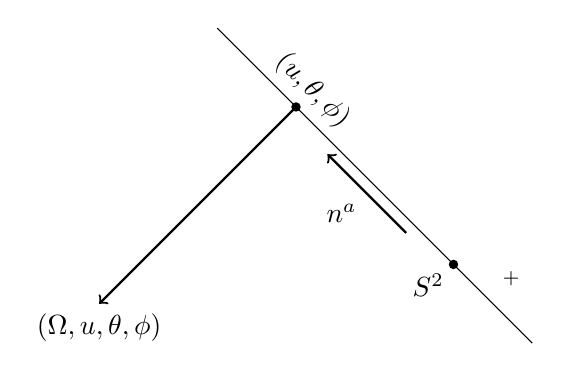
\begin{tikzpicture}
        \draw[thick,<-] (0.5,0.5) -- (3,3) node[at start,below] {\((\Omega,u,\theta,\phi)\)}; 
        \draw (2,4) -- (6,0);
        \fill (3,3) circle (0.06);
        \node[above, rotate=-45] at (3,3) {\((u,\theta,\phi)\)};
        \draw[thick,->] (4.4,1.4) -- (3.4,2.4) node[midway, below left] {\(n^a\)};
        \fill (5,1) circle (0.06) node[below left] {\(S^2\)};
        \node[above right] at (5.5,0.5) {\(\scri^+\)};
    \end{tikzpicture}
\end{figure}

Note that since \(\dd{\Omega}\) and \(n^a\) are null, we have \(\overline{g}_{uu} = \overline{g}_{\Omega\Omega} = 0\). Also, \(\delta^\mu_u=n^\mu = \overline{g}^{\mu\nu}(\dd{\Omega})_\nu = \overline{g}^{\mu\Omega}\). Examining the gauge condition (\(\dagger\)) we can deduce that the spherical part of the metric does not depend on \(u\). Thus we have
\begin{equation}
    \left.\overline{g}\right|_{\Omega=0} = 2\dd{u}\dd{\Omega} + \dd{\theta}^2 + \sin^2\theta\dd{\phi}^2.
\end{equation}
If we define \(r=\frac{1}{\Omega}\), then we obtain
\begin{align}
    g &= \Omega^{-2}\overline{g} = -2\dd{u}\dd{r}+r^2(\dd{\theta}^2 + \sin^2\theta\dd{\phi}^2) + \underbrace{\dots}_{\mathclap{\text{subleading as \(r \to \infty\)}}} \\
      &= -\dd{t}^2 + \dd{x}^2 + \dd{y}^2 + \dd{z}^2.
\end{align}

\begin{defn}
    \(\scri^+\) is \emph{complete} if in the gauge given by (\(\dagger\)), the generators of \(\scri^+\) are complete.
\end{defn}

\subsection{Definition of a black hole}

We have \(\scri^+ \subset \overline{\mathcal{M}}\). Consider the causal past of \(\scri^+\): \(J^-(\scri^+) \subset \overline{\mathcal{M}}\). \(\mathcal{M}\cap J^-(\scri^+)\) is the set of all points that can send a signal to \(\scri^+\).

\begin{defn}
    Let \((\mathcal{M},g)\) be a spacetime that is asymptotically flat at null infinity. We define the following:
    \begin{itemize}
        \item The \emph{black hole region} is \(\mathcal{B}=\mathcal{M}\setminus[\mathcal{M}\cap J^-(\scri^+)]\).
        \item The \emph{future event horizon} is \(\mathcal{H}^+ = \dot{\mathcal{B}} = \mathcal{M}\cap\dot{J}^-(\scri^+)\).
        \item The \emph{white hole region} is \(\mathcal{W}=\mathcal{M}\setminus[\mathcal{M}\cap J^+(\scri^-)]\).
        \item The \emph{past event horizon} is \(\mathcal{H}^- = \dot{\mathcal{W}} = \mathcal{M}\cap\dot{J}^+(\scri^-)\).
    \end{itemize}
\end{defn}
\begin{eg}
    In the Kruskal spacetime, we have:
    \begin{align}
        \mathcal{B} &= \{u\ge0\} & \mathcal{W} &= \{v\le0\} \\
        \mathcal{H}^+ &= \{u=0\} & \mathcal{H}^- &= \{v=0\}
    \end{align}
    \begin{figure}[H]
        \centering
        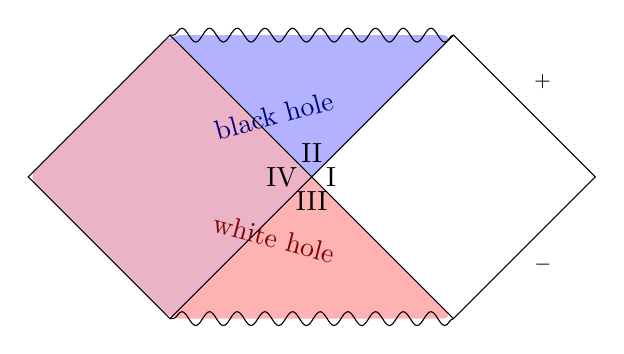
\begin{tikzpicture}[scale=0.6]
            \fill[rounded corners,blue!30] (3,3) -- (-3,3) -- (-6,0) -- (-3,-3) -- cycle;
            \fill[rounded corners,red!30] (3,-3) -- (-3,3) -- (-6,0) -- (-3,-3) -- cycle;
            \fill[rounded corners,purple!30] (0,0) -- (-3,3) -- (-6,0) -- (-3,-3) -- (0,0);

            \draw (3,3) -- (6,0) -- (3,-3) -- (-3,3) -- (-6,0) -- (-3,-3) -- cycle;
            \draw[decorate,decoration=snake] (3,3) -- (-3,3);
            \draw[decorate,decoration=snake] (3,-3) -- (-3,-3);

            \draw (0.1,0) node[right] {I};
            \draw (0,0.1) node[above] {II};
            \draw (0,-0.1) node[below] {III};
            \draw (-0.1,0) node[left] {IV};

            \node[above right] at (4.5,1.5) {\(\scri^+\)};
            \node[below right] at (4.5,-1.5) {\(\scri^-\)};

            \node[blue!50!black,rotate=15] at (-0.8,1.3) {black hole};
            \node[red!50!black,rotate=-15] at (-0.8,-1.3) {white hole};
        \end{tikzpicture}
    \end{figure}
    Note that \(\mathcal{H}^\pm\) are null hypersurfaces and their generators have no future endpoints.
\end{eg}

\begin{defn}
    An asymptotically flat spacetime \((\mathcal{M},g)\) is \emph{strongly asymptotically predictable} if there exists some open set \(\overline{V}\in\overline{\mathcal{M}}\) such that \(\overline{\mathcal{M}\cap J^-(\scri^+)} \subset \overline{V}\), and \((\overline{V},\overline{g})\) is globally hyperbolic.
\end{defn}

\begin{theorem}
    Suppose we have a strongly asymptotically predictable spacetime \((\mathcal{M},g)\) with Cauchy surfaces \(\Sigma_1\), \(\Sigma_2\) for \(\overline{V}\) such that \(\Sigma_2\subset I^+(\Sigma_1)\), and \(B\) a conncected component of \(\mathcal{B}\cap\Sigma_1\). Then \(J^+(B)\cap\Sigma_2\) is contained within a connected component of \(\mathcal{B}\cap\Sigma_2\).
\end{theorem}
\begin{proof}
    Suppose the black hole does split (bifurcate). Then there exist open sets \(O,O'\subset \Sigma_2\) such that \(O\cap O' = \varnothing\), \(J^+(B)\cap\Sigma_2\in O\cup O'\), \(J^+(B)\cap O \ne \varnothing \ne J^+(B)\cap O'\).
    \begin{figure}[H]
        \centering
        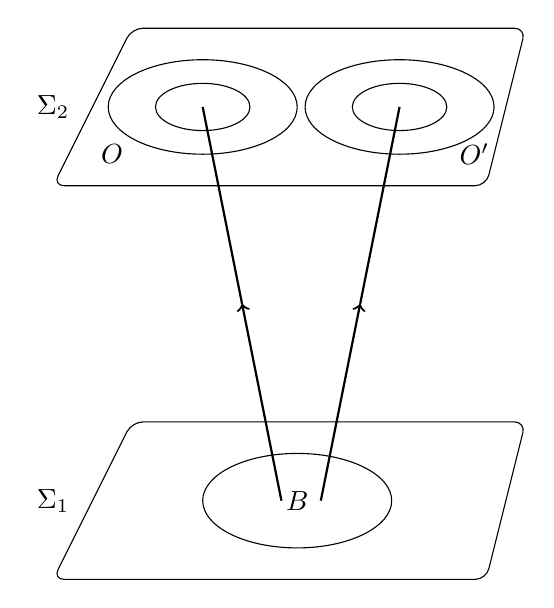
\begin{tikzpicture}
            \draw[rounded corners] (0,0) -- (1,2) -- (6,2) -- (5.5,0) -- cycle;
            \draw[rounded corners] (0,5) -- (1,7) -- (6,7) -- (5.5,5) -- cycle;

            \node at (0,1) {\(\Sigma_1\)};
            \node at (0,6) {\(\Sigma_2\)};

            \draw (3.1,1) node {\(B\)} ellipse (1.2 and 0.6);

            \draw (1.9,6) ellipse (1.2 and 0.6);
            \draw (4.4,6) ellipse (1.2 and 0.6);

            \draw (1.9,6) ellipse (0.6 and 0.3);
            \draw (4.4,6) ellipse (0.6 and 0.3);

            \node at (0.75,5.4) {\(O\)};
            \node at (5.35,5.4) {\(O'\)};

            \draw[thick,->] (2.9,1) -- (2.4,3.5);
            \draw[thick] (2.4,3.5) -- (1.9,6);
            \draw[thick,->] (3.4,1) -- (3.9,3.5);
            \draw[thick] (3.9,3.5) -- (4.4,6);
        \end{tikzpicture}
    \end{figure}
    Note that \(B\cap I^-(O) \ne \varnothing \ne B\cap I^-(O')\), and \(B\subset I^-(O)\cup I^-(O)\). If \(p\) is a point in \(B\) such that \(p\in I^-(O)\) and \(p\in I^-(O')\), then we can divide the future-directed timelike geodesics from \(p\) into 2 sets depending on which of \(O\), \(O'\) they reach. Thus we can divide the timelike vectors at \(p\) into 2 disjoint sets, but this is a contradiction since the future light cone is connected. So there does not exist such a \(p\), so \(B\cap I^-(O)\cap I^-(O')=\varnothing\), and \(B=[B\cap I^-(O)]\cup[B\cap I^-(O')]\) is a disjoint union, contradicting the connectedness of \(B\).
\end{proof}

\subsection{Weak cosmic censorship conjecture}
In the Kruskal spacetime, the white hole singularity is ``naked'', i.e.\ it is visbile to \(\scri^+\). For \(M<0\) Schwarzschild we have the Penrose diagram
\begin{figure}[H]
    \centering
    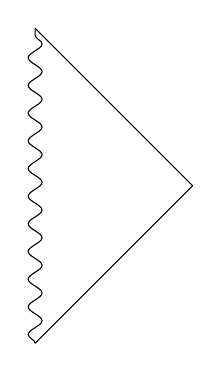
\begin{tikzpicture}
        \draw (0,0) -- (2,2) -- (0,4);
        \draw[decorate,decoration=snake] (0,0) -- (0,4);
    \end{tikzpicture}
\end{figure}
and we see that the \(r=0\) singularity is also naked here.

It is reasonable to ask whether gravitational collapse could lead to a naked singularity. In fact we have the following conjecture (\emph{weak cosmic censorship}):
\begin{quote}
    Suppose \((\Sigma,h_{ab},K^{ab})\) is a geodesically complete, asymptotically flat initial data set, and that matter fields obey hyperbolic equations and the dominant energy condition. Then, generically, the maximal development is asymptotically flat (so \(\scri^+\) is complete) and strongly asymptotically predictable.
\end{quote}

Note that the strong and weak censorship conjectures are logically distinct.

\subsection{Apparent horizon}
\begin{theorem}
    If \((\mathcal{M},g)\) is a strongly asymptotically predictable spacetime satisfying the null energy condition and Einstein's equations that contains a trapped surface \(T\), then \(T\subset\mathcal{B}\).
\end{theorem}
Consider a 1-parameter family of Cauchy surfaces \(\Sigma_t\). When we say the \emph{black hole region at time \(t\)} or the \emph{event horizon at time \(t\)}, we are referring to the sets \(B_t = \mathcal{B}\cap \Sigma_t\) and \(H_t = \mathcal{H}\cap\Sigma_t\) respectively.
\begin{defn}
    The \emph{trapped region} at time \(t\) is \(\tau_t = \{p\in\Sigma_t \st \Exists \text{trapped \(S\) with \(p \in S\subset\Sigma_t\)}\}\). The \emph{apparent horizon} is \(\mathcal{A}_t = \dot{\tau}_t\).
\end{defn}
Note that we have \(\tau_t\in B_t\), and \(\mathcal{A}_t \in B_t\). Also \(\mathcal{A}_t\) is on or inside \(H_t\), and \(\mathcal{A}_t\) is marginally trapped.

\section{Charged Black Holes}
\lecture{15/02/16}
\subsection{The Reissner-Nordstrom solution}
Recall the Einstein-Maxwell action
\begin{equation}
    S = \frac{1}{16\pi}\int\dd[4]{x}\sqrt{-g}(R-F^{ab}F_{ab}) \qq{where} F=\dd{A}.
\end{equation}
This action gives the following equations of motion:
\begin{equation}
    R_{ab}-\frac{1}{2}Rg_{ab} = 2\left(F_{ac}F\indices{_b^c} - \frac{1}{4}F^{cd}F_{cd}g_{ab}\right), \quad \nabla^b F_{ab} = 0
\end{equation}

\begin{theorem}
    The unique spherically symmetric solution with non-constant area-radius function \(r\) is the Reissner-Nordstrom solution, given by
    \begin{equation}
        \dd{s}^2 = -\left(1-\frac{2M}{r} + \frac{e^2}{r^2}\right)\dd{t}^2 + \left(1-\frac{2M}{r}+\frac{e^2}{r^2}\right)^{-1}\dd{r}^2 + r^2\dd{\Omega}^2
    \end{equation}
    and
    \begin{equation}
        A = -\frac{Q}{r}\dd{t}-P\cos\theta\dd{\phi}
    \end{equation}
    where \(e=\sqrt{Q^2+P^2}\).
\end{theorem}
The Reissner-Nordstrom solution has three parameters. We identify them as the mass \(M\), electric charge \(Q\), and magnetic charge \(P\) of the black hole. It is static with a timelike KVF \(k=\pdv{t}\), and it is asymptotically flat at null infinity.

To make the metric easier to write down, we define \(\Delta = r^2-2Mr + e^2 = (r-r_+)(r-r_-)\) where \(r_\pm=M\pm\sqrt{M^2-e^2}\). Then
\begin{equation}
    \dd{s}^2 = - \frac{\Delta}{r^2}\dd{t}^2 + \frac{r^2}{\Delta}\dd{r}^2 + r^2\dd{\Omega}^2.
\end{equation}
Consider \(M^2<e^2\). Then \(\Delta > 0\) for all \(r>0\), and we have a naked curvature singularity at \(r=0\). Thus we will ignore this case and assume from now on that \(M>e\) (confer \(M<0\) Schwarzschild).

\subsection{Eddington-Finklestein coordinates}
We define \(r_*\) by \(\dd{r_*} = \frac{r^2}{\Delta}\dd{r}\). If we want we can solve this to obtain
\begin{equation}
    r_* = r + \frac{1}{2\kappa_+}\log\left|\frac{r-r_+}{r_+}\right| + \frac{1}{2\kappa_-}\log\left|\frac{r-r_-}{r_-}\right| + \text{constant}
\end{equation}
where \(\kappa_\pm = \frac{r_\pm-r_\mp}{2r_\pm^2}\). Let \(u = t-r_*\) and \(v = t+r_*\). Then we can write the metric in ingoing E-F coordinates \((v,r,\theta,\phi)\) as
\begin{equation}
    \dd{s}^2 = -\frac{\Delta}{r^2}\dd{v}^2 + 2\dd{v}\dd{r} + r^2\dd{\Omega}^2.
\end{equation}
This is smooth for all \(r>0\), and \(\det g \ne 0\), so we can extend spacetime to the region \(0<r<r_+\). There is a curvature singularity at \(r=0\). Since \(\dd{r}\) is null when \(g^{rr} = \frac{\Delta}{r^2} = 0\), we have that \(r=r_\pm\) are null hypersurfaces. It can be shown that \(r\) decreases along any future-directed causal curve in \(r_-<r<r_+\). ?Hence we have a black hole region \(r\le r_+\) with event horizon \(\mathcal{H}^+\) given by \(r=r_+\).

We can carry out a similar argument in \((u,r,\theta,\phi)\) to show that there is a white hole region with \(r<r_+\).

\subsection{Kruskal-like coordinates}
Now let \(U^\pm=-e^{-\kappa_\pm u}\) and \(V^\pm = \pm e^{\kappa_\pm v}\). In \(r<r_+\) we have coordinates \((U^+,V^+,\theta,\phi)\) and the metric takes the form
\begin{equation}
    \dd{s}^2 = -\frac{r_+r_-}{\kappa_+^2r^2}e^{-2\kappa_+r}\left(\frac{r-r_-}{r_-}\right)^{1+\frac{\kappa_+}{|\kappa_-|}}\dd{U^+}\dd{V^+} + r^2\dd{\Omega}^2
\end{equation}
where \(r(U^+,V^+)\) is defined by 
\begin{equation}
    -U^+V^+ = e^{2\kappa_+ r}\left(\frac{r-r_+}{r_+}\right)\left(\frac{r_-}{r-r_-}\right)^{\frac{\kappa_+}{|\kappa_-|}}.
\end{equation}
Initially \(U^+<0\) and \(V^+>0\), but we can analytically continue to \(U^+\ge 0\) or \(V^+\le 0\).
\begin{figure}[H]
    \centering
    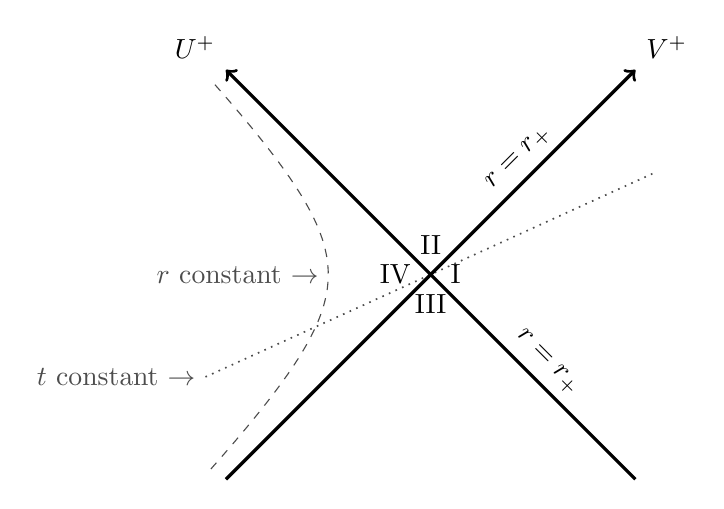
\begin{tikzpicture}[scale=1.3]
        \begin{scope}[black!70]
            \draw[domain=-1.9:1.9,smooth,variable=\x,dashed] plot({-sqrt(1+\x*\x))},{\x});
            \node[left] at (-1,0) {\(r\) constant \(\rightarrow\)};

            \draw[dotted, semithick] (-2.2,-1) -- (2.2,1) node[left, at start] {\(t\) constant \(\rightarrow\)};
        \end{scope}

        \draw (0.1,0) node[right] {I};
        \draw (0,0.1) node[above] {II};
        \draw (0,-0.1) node[below] {III};
        \draw (-0.1,0) node[left] {IV};

        \draw[very thick,->] (-2,-2) -- (2,2) node[above right] {\(V^+\)} node[near end, above, sloped] {\(r=r_+\)};
        \draw[very thick,->] (2,-2) -- (-2,2) node[above left] {\(U^+\)} node[near start, above, sloped] {\(r=r_+\)};
    \end{tikzpicture}
\end{figure}
Note \(k^a=0\) at \(U^+=V^+=0\). Ingoing radial null geodesics have \(r\to r_-\) (\(U^+V^+\to-\infty\)) in finite affine parameter.

Unlike the Schwarzschild solution, we can continue to extend the spacetime. In region II, let \(t = v-r_*\) and \(u=t-r_* = v-2r_*\). We use coordinates \((U^-,V^-,\theta,\phi)\) where \(U^-,V^-<0\). The metric is
\begin{equation}
    \dd{s}^2 = -\frac{r_+r_-}{\kappa_-^2r^2}e^{-2|\kappa_-|r}\left(\frac{r_+-r}{r_+}\right)^{1+\frac{|\kappa_-|}{\kappa_+}}\dd{U^-}\dd{V^-} + r^2\dd{\Omega}^2
\end{equation}where \(r(U^-,V^-)\) is defined by 
\begin{equation}
    -U^+V^+ = e^{2|\kappa_-| r}\left(\frac{r-r_-}{r_-}\right)\left(\frac{r_+}{r_+-r}\right)^{\frac{|\kappa_-|}{\kappa_+}}.
\end{equation}
\lecture{17/02/16}
We analytically continue to \(U^-,V^-\ge0\) to find new regions V, VI and III\({}'\).
\begin{figure}[H]
    \centering
    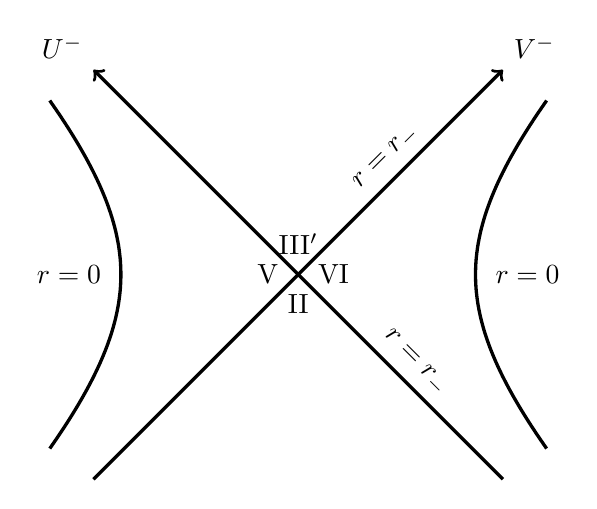
\begin{tikzpicture}[scale=1.3]
        \draw (0.1,0) node[right] {VI};
        \draw (0,0.1) node[above] {III\({}'\)};
        \draw (0,-0.1) node[below] {II};
        \draw (-0.1,0) node[left] {V};

        \draw[very thick,->] (-2,-2) -- (2,2) node[above right] {\(V^-\)} node[near end, above, sloped] {\(r=r_-\)};
        \draw[very thick,->] (2,-2) -- (-2,2) node[above left] {\(U^-\)} node[near start, above, sloped] {\(r=r_-\)};

        \begin{scope}[rotate=90]
            \draw[domain=-1.7:1.7,smooth,variable=\x,very thick] plot({\x},{sqrt(3+\x*\x))});
            \node[left] at (0,{sqrt(3)+0.1}) {\(r=0\)};
            \draw[domain=-1.7:1.7,smooth,variable=\x,very thick] plot({\x},{-sqrt(3+\x*\x))});
            \node[right] at (0,{-sqrt(3)-0.1}) {\(r=0\)};
        \end{scope}
    \end{tikzpicture}
\end{figure}
Note that III\({}'\) is isometric to III, so we can use coordinates \(({U^+}',{V^+}')\) an extend out to new regions I\({}'\), II\({}'\) and IV\({}'\).
\begin{figure}[H]
    \centering
    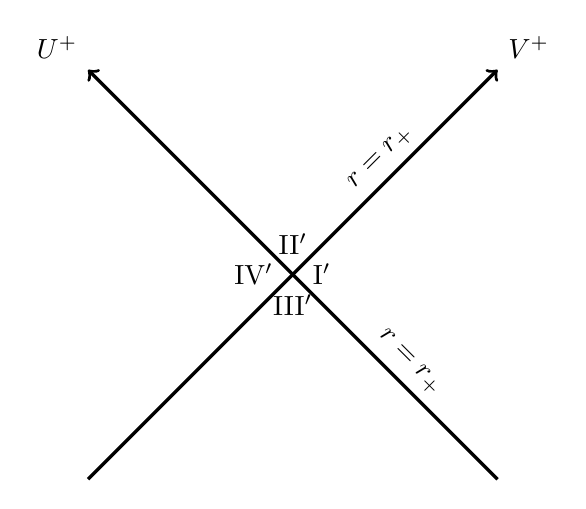
\begin{tikzpicture}[scale=1.3]
        \draw (0.1,0) node[right] {I\({}'\)};
        \draw (0,0.1) node[above] {II\({}'\)};
        \draw (0,-0.1) node[below] {III\({}'\)};
        \draw (-0.1,0) node[left] {IV\({}'\)};

        \draw[very thick,->] (-2,-2) -- (2,2) node[above right] {\(V^+\)} node[near end, above, sloped] {\(r=r_+\)};
        \draw[very thick,->] (2,-2) -- (-2,2) node[above left] {\(U^+\)} node[near start, above, sloped] {\(r=r_+\)};
    \end{tikzpicture}
\end{figure}
We can repeat this process indefinitely. We can also draw a Penrose diagram of the extended spacetime:
\begin{figure}[H]
    \centering
    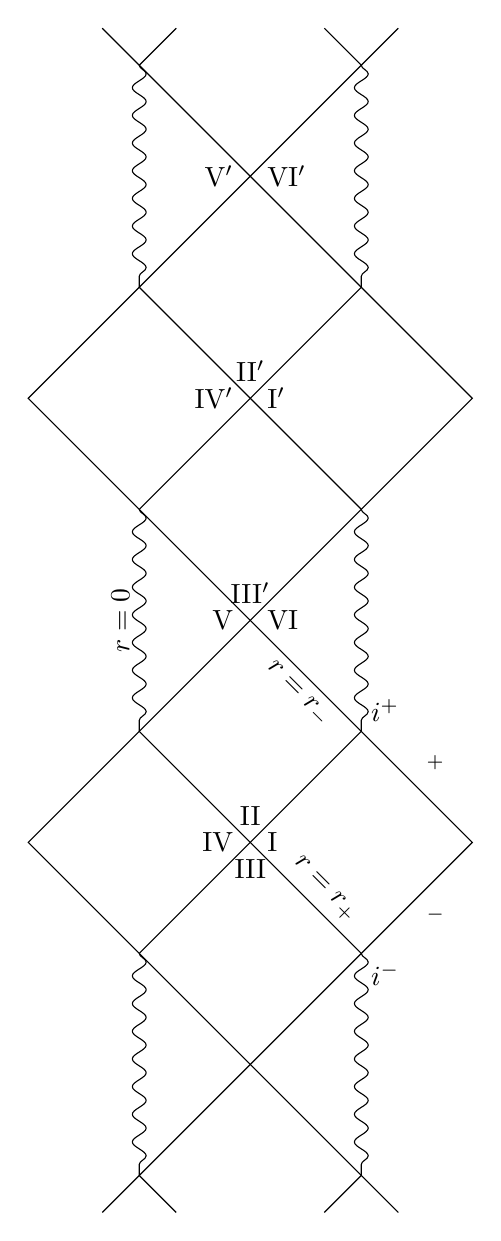
\begin{tikzpicture}[scale=0.94]
        \draw (2,8) -- (-3,3) -- (3,-3) -- (-2,-8);
        \draw (-2,8) -- (3,3) -- (-3,-3) -- (2,-8);
        \draw (1.5,1.5) -- (-1.5,4.5);
        \draw (-1.5,1.5) -- (1.5,4.5);
        \draw (1.5,-1.5) -- (-1.5,-4.5);
        \draw (-1.5,-1.5) -- (1.5,-4.5);
        \draw (1.5,7.5) -- (1,8);
        \draw (-1.5,7.5) -- (-1,8);
        \draw (1.5,-7.5) -- (1,-8);
        \draw (-1.5,-7.5) -- (-1,-8);
        \draw[decorate,decoration=snake] (1.5,7.5) -- (1.5,4.5);
        \draw[decorate,decoration=snake] (-1.5,7.5) -- (-1.5,4.5);
        \draw[decorate,decoration=snake] (1.5,1.5) -- (1.5,-1.5);
        \draw[decorate,decoration=snake] (-1.5,1.5) -- (-1.5,-1.5);
        \draw[decorate,decoration=snake] (1.5,-4.5) -- (1.5,-7.5);
        \draw[decorate,decoration=snake] (-1.5,-4.5) -- (-1.5,-7.5);

        \begin{scope}[shift={(0,6)}]
            \draw (0.1,0) node[right] {VI\({}'\)};
            \draw (-0.1,0) node[left] {V\({}'\)};
        \end{scope}
        \begin{scope}[shift={(0,3)}]
            \draw (0.1,0) node[right] {I\({}'\)};
            \draw (0,0.1) node[above] {II\({}'\)};
            \draw (-0.1,0) node[left] {IV\({}'\)};
        \end{scope}
        \begin{scope}
            \draw (0.1,0) node[right] {VI};
            \draw (0,0.1) node[above] {III\({}'\)};
            \draw (-0.1,0) node[left] {V};
        \end{scope}
        \begin{scope}[shift={(0,-3)}]
            \draw (0.1,0) node[right] {I};
            \draw (0,0.1) node[above] {II};
            \draw (0,-0.1) node[below] {III};
            \draw (-0.1,0) node[left] {IV};
        \end{scope}

        \node[above,rotate=-45] at (0.82,-3.82) {\(r=r_+\)};
        \node[below,rotate=-45] at (0.82,-0.82) {\(r=r_-\)};
        \node[above,rotate=90] at (-1.5,0) {\(r=0\)};
        \node[above right] at (2.25,-2.25) {\(\scri^+\)};
        \node[below right] at (2.25,-3.75) {\(\scri^-\)};
        \node[above right] at (1.5,-1.5) {\(i^+\)};
        \node[below right] at (1.5,-4.5) {\(i^-\)};
    \end{tikzpicture}
\end{figure}

\subsection{Extreme Reissner-Nordstrom}
\begin{wrapfigure}{l}{0.5\linewidth}
    \centering
    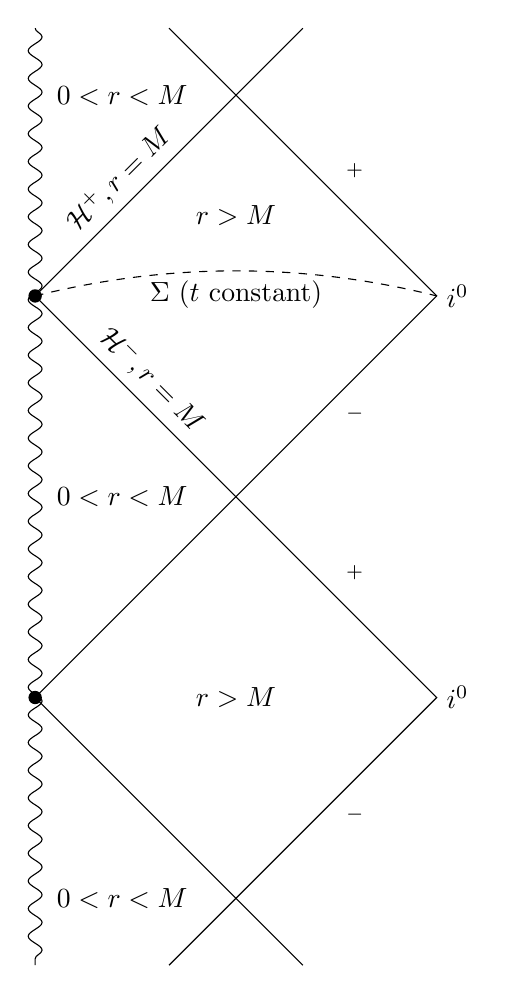
\begin{tikzpicture}[scale=0.85]
        \draw (4,7) -- (0,3) -- (6,-3) -- (2,-7);
        \draw (2,7) -- (6,3) -- (0,-3) -- (4,-7);
        \draw[decorate,decoration=snake] (0,7) -- (0,-7);
        \fill (0,3) circle (0.1);
        \fill (0,-3) circle (0.1);

        \node at (1.3,6) {\(0 < r < M\)};
        \node at (1.3,0) {\(0 < r < M\)};
        \node at (1.3,-6) {\(0 < r < M\)};

        \node[right] at (6,3) {\(i^0\)};
        \node[right] at (6,-3) {\(i^0\)};

        \node[above right] at (4.5,4.5) {\(\scri^+\)};
        \node[above right] at (4.5,-1.5) {\(\scri^+\)};

        \node[below right] at (4.5,1.5) {\(\scri^-\)};
        \node[below right] at (4.5,-4.5) {\(\scri^-\)};
        
        \node[rotate=-45, above] at (1.5,1.5) {\(\mathcal{H}^-, r=M\)};
        \node[rotate=45, above] at (1.5,4.5) {\(\mathcal{H}^+, r=M\)};

        \draw[dashed] (0,3) .. controls (2,3.5) and (4,3.5) .. (6,3) node[midway, below] {\(\Sigma\) (\(t\) constant)};

        \node at (3,4.2) {\(r>M\)};
        \node at (3,-3) {\(r>M\)};
    \end{tikzpicture}
\end{wrapfigure}
The Reissner-Nordstrom solution with \(M=e\) is known as \emph{extreme} RN. In this case \(r_+=r_-=M\) and the metric takes the simple form
\begin{equation}
    \dd{s}^2 = -\left(1-\frac{M}{r}\right)^2\dd{t}^2 + \left(1-\frac{M}{r}\right)^{-2}\dd{r}^2 + r^2\dd{\Omega}^2.
\end{equation}
We can introduce Eddington-Finklestein coordinates in \(r>M\) with \(\dd{r_*} = \frac{\dd{r}}{(1-M/r)^2}\) and \(v=t+r_*\) to obtain
\begin{equation}
    \dd{s}^2 = -\left(1-\frac{M}{r}\right)^2\dd{v}^2 + 2\dd{v}\dd{r} + r^2\dd{\Omega}^2.
\end{equation}

Extreme RN has the following Penrose diagram as shown to the left.

We have \(\mathcal{H}^\pm = H^\pm(\Sigma)\). The proper length of a line from \(r=r_0>M\) to \(r=M\) with \(t,\theta,\phi\) constant diverges:
\begin{equation}
    \int^{r_0}_M \frac{\dd{r}}{1-M/r}
\end{equation}
If we set \(r=M(1+\lambda)\) where \(\lambda\) is small, we obtain
\begin{equation}
    \dd{s}^2 \approx \underbrace{- \lambda^2\dd{t}^2 + M^2 \frac{\dd{\lambda^2}}{\lambda^2}}_{\text{AdS}_2} + \underbrace{M^2 \dd{\Omega}^2}_{S^2}.
\end{equation}
The spacetime looks like an infinite throat as we approach \(r=M\):
\begin{figure}[H]
    \centering
    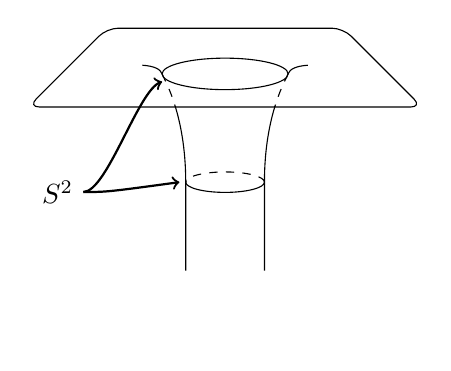
\begin{tikzpicture}
        \draw[rounded corners, shift={(0,0.08)}] (0,3) -- (5,3) -- (4,4) -- (1,4) -- cycle;

        \draw (2.5,3.5) ellipse (0.8 and 0.2);
        \begin{scope}[shift={(0,2.125)},yscale=0.26]
            \draw (3,0) arc (0:-180:0.5);
            \draw[dashed] (3,0) arc (0:180:0.5);
        \end{scope}
        
        \begin{scope}
            \clip[shift={(0,0.08)}] (0,3) rectangle (5,0);
            \draw (3.3,3.5) .. controls (3.28,3.44) and (3,3) .. (3,2.125) -- (3,1);
            \draw (1.7,3.5) .. controls (1.72,3.44) and (2,3) .. (2,2.125) -- (2,1);
        \end{scope}
        \begin{scope}[dashed]
            \clip[shift={(0,0.08)}] (0,3) rectangle (5,4);
            \draw (3.3,3.5) .. controls (3.28,3.44) and (3,3) .. (3,2.125)
                            .. controls (3,1.25) and (3.28,0.71) .. (3.3,0.65);
            \draw (1.7,3.5) .. controls (1.72,3.44) and (2,3) .. (2,2.125)
                            .. controls (2,1.25) and (1.72,0.71) .. (1.7,0.65);
        \end{scope}

        \draw (3.3,3.5) .. controls (3.32,3.56) and (3.4,3.6) .. (3.55,3.61);
        \draw (1.7,3.5) .. controls (1.68,3.56) and (1.6,3.6) .. (1.45,3.61);

        \draw[->, thick] (0.7,2) node[left] {\(S^2\)} .. controls (1,2) and (1.4,3.3) .. (1.7,3.4);
        \draw[->, thick] (0.7,2) .. controls (1,2) .. (1.92,2.125);
    \end{tikzpicture}
\end{figure}

\subsection{Majumdar-Papapetrou solutions}
We introduce a new radial coordinate \(\rho = r-M\), and assume that the magnetic charge vanishes, \(P=0\). Then the metric takes the form
\begin{equation}
    \dd{s}^2 = -H^{-2}\dd{t}^2 + H^2(\dd{\rho}^2 + \rho^2\dd{\Omega}^2)
\end{equation}
where \(H=1+\frac{M}{\rho}\). This is a special case of the Majumdar-Papapetrou solution
\begin{equation}
    \dd{s}^2 = -H(\vb{x})^{-2}\dd{t}^2 + H(\vb{x})^2 (\dd{x}^2 + \dd{y}^2 + \dd{z}^2), \quad A = H^{-1}\dd{t},
\end{equation}
where \(\vb{x} = (x,y,z)\) and \(H\) is harmonic, \(\nabla^2H=0\). The fact that the equation for \(H\) is linear allows a large family of exact solutions to exist.

An interesting case arises when we set \(H = 1 + \sum^N_{i=1}\frac{M_i}{\vb{x}-\vb{x_i}}\). This leads to a static solution with \(N\) extreme RN black holes. The physical interpretation of this is that since \(M_i=Q_i\) there is an exact balance of electrostatic repulsion and gravitational attraction.

\section{Rotating Black Holes}
\lecture{19/02/16}
We need to slightly modify our definitions of stationary and static.
\begin{defn}
    An asymptotically flat spacetime is \emph{stationary} if there exists a KVF \(k^a\) that is timelike in a neighbourhood of \(\scri^\pm\), and \emph{static} if \(k^a\) is also hypersurface orthogonal.
\end{defn}
It is conventional to normalise such that \(k^2\to-1\) at \(\scri^\pm\).
\begin{defn}
    An asymptotically flat spacetime is \emph{stationary and axisymmetric} if:
    \begin{itemize}
        \item It is stationary.
        \item There exists a KVF \(m^a\) that is spacelike near \(\scri^\pm\).
        \item \(m^a\) generates a 1-parameter group of isometries isomorphic to U(1).
        \item \([k,m]=0\).
    \end{itemize}
\end{defn}
We can choose coordinates such that \(k=\pdv{t}\), \(m=\pdv{\phi}\), \(\phi \sim \phi+2\pi\).
\begin{theorem}
    If \((\mathcal{M},g)\) is a static, asymptotically flat, vacuum spacetime that contains a black hole and is regular on and outside \(\mathcal{H}^+\), then \((\mathcal{M},g)\) is isometric to Schwarzschild spacetime.
\end{theorem}
\begin{theorem}
    If \((\mathcal{M},g)\) is a stationary, non-static, asymptotically flat spacetime that is an analytic solution of the Einstein-Maxwell equations and is regular on and outside \(\mathcal{H}^+\), then \((\mathcal{M},g)\) is stationary and axisymmetric.
\end{theorem}
\begin{theorem}
    If \((\mathcal{M},g)\) is a stationary, axisymmetric, asymptotically flat, vacuum spacetime that is regular on and outside connected \(\mathcal{H}^+\), then \((\mathcal{M},g)\) belongs to the Kerr family of solutions.
\end{theorem}

\subsection{The Kerr-Newman solution}

In Boyer-Lindquist coordinates, the Kerr-Newman solution is as follows:
\begin{align}
    \dd{s}^2 &= - \frac{\Delta-a^2\sin^2\theta}{\Sigma}\dd{t}^2 - 2a\sin^2\theta\frac{r^2+a^2-\Delta}{\Sigma}\dd{t}\dd{\phi} \\
             &\qquad + \frac{(r^2+a^2)^2 - \Delta a^2\sin^2\theta}{\Sigma}\sin^2\theta\dd{\phi}^2 + \frac{\Sigma}{\Delta}\dd{r}^2 + \Sigma\dd{\theta}^2 \\
    A &= - \frac{1}{\Sigma}\left[Qr(\dd{t}-a\sin^2\theta\dd{\phi}) + P\cos\theta(a\dd{t}-(r^2+a^2)\dd{\phi})\right] \\
    \text{where } \Sigma &= r^2 + a^2\cos^2\theta,\quad \Delta = r^2-2Mr + a^2 + e^2,\quad e=\sqrt{Q^2+P^2}
\end{align}
This solution is stationary and axisymmetric with KVFs \(k=\pdv{t}\) and \(m=\pdv{\phi}\). It also permits a discrete isometry \(t\to-t,\phi\to-\phi\). It has four parameters: the mass \(M\), electric charge \(Q\), magnetic charge \(P\), and angular momentum \(J=aM\) (these names will be justified in the next section). Under \(\phi\to-\phi\), we have \(a\to-a\), so w.l.o.g.\ we can assume that \(a\ge0\).

\subsection{The Kerr solution}
The Kerr solution is the Kerr-Newman solution with \(Q=P=e=0\). In this case we have \(\Delta = (r-r_+)(r-r_-)\), where \(r_\pm = M\pm\sqrt{M^2-a^2}\). If \(M^2<a^2\) we get a naked singularity, so we will assume \(M>|a|\). The metric is singular at \(\theta=0,\pi\) in the ordinary spherical way. We also have singularities at \(\Delta=0\) and at \(\Sigma=0\). These are just coordinate singularities. To show this, define new coordinates \(v\) and \(\chi\) by
\begin{equation}
    \dd{v} = \dd{t}+\frac{r^2+a^2}{\Delta}\dd{r} \qq{and} \dd{\chi}=\dd{\phi} + \frac{a}{\Delta}\dd{r} (\chi\sim\chi+2\pi).
\end{equation}
In these coordinates we have \(k=\pdv{v}\) and \(m=\pdv{\chi}\). \emph{Kerr coordinates} are \((v,r,\theta,\chi)\), and the metric becomes
\begin{align}
    \dd{s}^2 &= - \frac{\Delta-a^2\sin^2\theta}{\Sigma}\dd{v}^2 + 2\dd{v}\dd{r}-2a^2\sin^2\theta\frac{r^2+a^2-\Delta}{\Sigma}\dd{v}\dd{\chi} \\
             &\qquad -2a\sin^2\theta\dd{\chi}\dd{r} + \frac{(r^2+a^2)^2-\Delta a^2\sin^2\theta}{\Sigma}\sin^2\theta\dd{\chi}^2+\Sigma\dd{\theta}^2.
\end{align}
This metric can be analytically extended into \(0<r<r_+\).
\begin{lemma}
    \(r=r_+\) is a null hypersurface with normal \(xi^a=k^a + \Omega_H m^a\) where \(\Omega_H = \frac{a}{r^2+a^2}\).
\end{lemma}
(This can be proven by showing that \(\left.\xi_\mu\dd{x}^\mu\right|_{r=r_+} \propto \dd{r}\), so \(\xi_a \perp \{r=r_+\}\) and \(\left.\xi_\mu\xi^\mu\right|_{r=r_+} = 0\).)

\(r\le r_+\) is the spacetime's black hole region \(\mathcal{B}\), and \(r=r_+\) is its event horizon \(\mathcal{H}^+\).

\lecture{22/02/16}
In Boyer-Lindquist coordinates, \(\xi=\pdv{t}+\Omega_H\pdv{\phi}\), and we have \(\xi^\mu\partial_\mu(\phi-\Omega_H t)=0\), so \(\phi= \Omega_H t + \text{constant}\) on orbits of \(\xi^a\). Thus the generators of \(\mathcal{H}^+\) rotate with angular velocity \(\Omega_H\) with respect to a stationary observer at \(\infty\). We say that \(\Omega_H\) is the angular velocity of the black hole.

\subsection{Maximal analytic extension}
Kerr coordinates are analagous to the ingoing E-F coordinates used for the RN black hole. We can similarly find outgoing coordinates to find a white hole region, and then construct a Kruskal like extension containg the regions I, II, III, IV. Similar to RN, we can extend II to new regions V, VI, III\({}'\), etc. One key difference is that \(r=0\) becomes a ``ring'' singularity, leading to a new flat region of space.

The Kerr solution has no spherical symmetry, so we cannot draw a Penrose diagram. Instead we will just refer to submanifolds. One submanifold is the ``axis'' given by \(\theta=0 \text{ or } \pi\). This is two dimensional, since we fix \(\theta\), and \(\phi\) is meaningless on the axis. We can construct a Penrose-like diagram for the axis:

\begin{figure}[H]
    \centering
    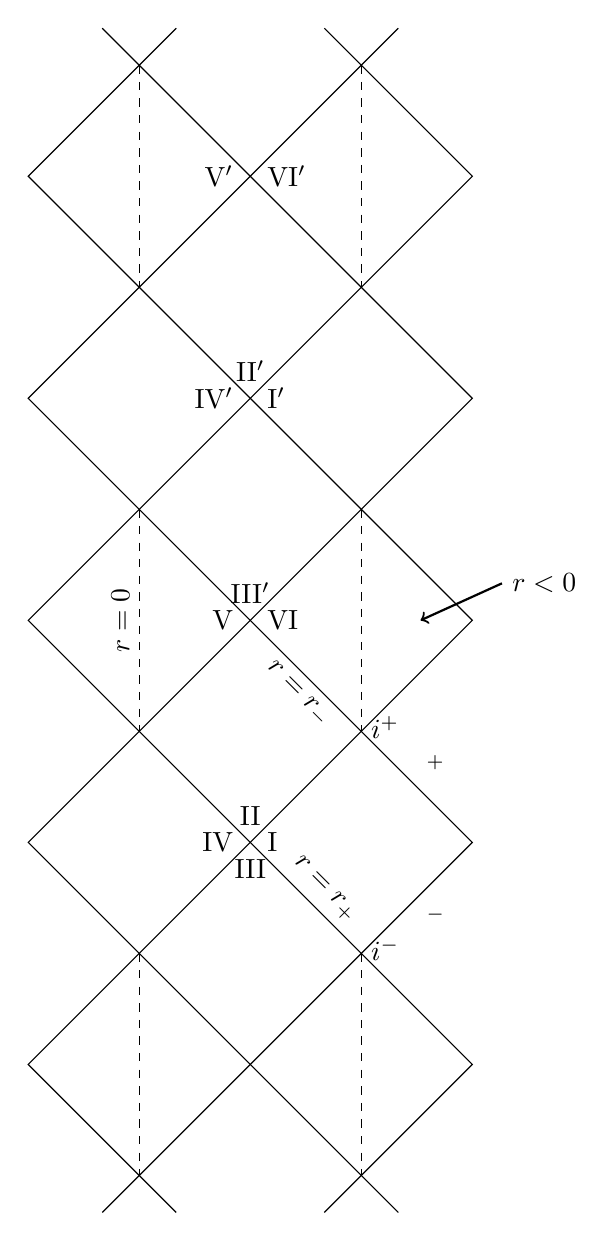
\begin{tikzpicture}[scale=0.94]
        \draw (2,8) -- (-3,3) -- (3,-3) -- (-2,-8);
        \draw (-2,8) -- (3,3) -- (-3,-3) -- (2,-8);
        \draw (1,8) -- (3,6) -- (-3,0) -- (3,-6) -- (1,-8);
        \draw (-1,8) -- (-3,6) -- (3,0) -- (-3,-6) -- (-1,-8);
        \draw[dashed] (1.5,7.5) -- (1.5,4.5);
        \draw[dashed] (-1.5,7.5) -- (-1.5,4.5);
        \draw[dashed] (1.5,1.5) -- (1.5,-1.5);
        \draw[dashed] (-1.5,1.5) -- (-1.5,-1.5);
        \draw[dashed] (1.5,-4.5) -- (1.5,-7.5);
        \draw[dashed] (-1.5,-4.5) -- (-1.5,-7.5);

        \begin{scope}[shift={(0,6)}]
            \draw (0.1,0) node[right] {VI\({}'\)};
            \draw (-0.1,0) node[left] {V\({}'\)};
        \end{scope}
        \begin{scope}[shift={(0,3)}]
            \draw (0.1,0) node[right] {I\({}'\)};
            \draw (0,0.1) node[above] {II\({}'\)};
            \draw (-0.1,0) node[left] {IV\({}'\)};
        \end{scope}
        \begin{scope}
            \draw (0.1,0) node[right] {VI};
            \draw (0,0.1) node[above] {III\({}'\)};
            \draw (-0.1,0) node[left] {V};
        \end{scope}
        \begin{scope}[shift={(0,-3)}]
            \draw (0.1,0) node[right] {I};
            \draw (0,0.1) node[above] {II};
            \draw (0,-0.1) node[below] {III};
            \draw (-0.1,0) node[left] {IV};
        \end{scope}

        \node[above,rotate=-45] at (0.82,-3.82) {\(r=r_+\)};
        \node[below,rotate=-45] at (0.82,-0.82) {\(r=r_-\)};
        \node[above,rotate=90] at (-1.5,0) {\(r=0\)};
        \node[above right] at (2.25,-2.25) {\(\scri^+\)};
        \node[below right] at (2.25,-3.75) {\(\scri^-\)};
        \node[right] at (1.5,-1.45) {\(i^+\)};
        \node[right] at (1.5,-4.45) {\(i^-\)};
        
        \draw[<-,thick] (2.3,0) -- (3.4,0.5) node[right]{\(r<0\)};
    \end{tikzpicture}
\end{figure}

Note that the Kerr solution just describes the final state of a rotating black hole; it has nothing to do with collapse.

If \(M=a\), we obtain \emph{extreme} Kerr, similar to extreme RN.

\subsection{Ergosphere/Penrose process}
We have
\begin{equation}
    k^2 = g_{tt} = - \left(1-\frac{2Mr}{r^2+a^2\cos^2\theta}\right).
\end{equation}
Therefore \(k\) is timelike in region I when \(r^2-2Mr+a^2\cos^2\theta>0\), i.e.\ when \(r > M + \sqrt{M^2-a^2\cos^2\theta}\) (this is the root in region I).

There is a region outside the event horizon in which \(k\) is spacelike, and this is known as the \emph{ergosphere}:
\begin{equation}
    M+\sqrt{M^2-a^2} = r_+ < r < M + \sqrt{M^2-a^2\cos^2\theta}
\end{equation}
The boundary of the ergosphere is called the \emph{ergosurface}.

\begin{figure}[H]
    \centering
    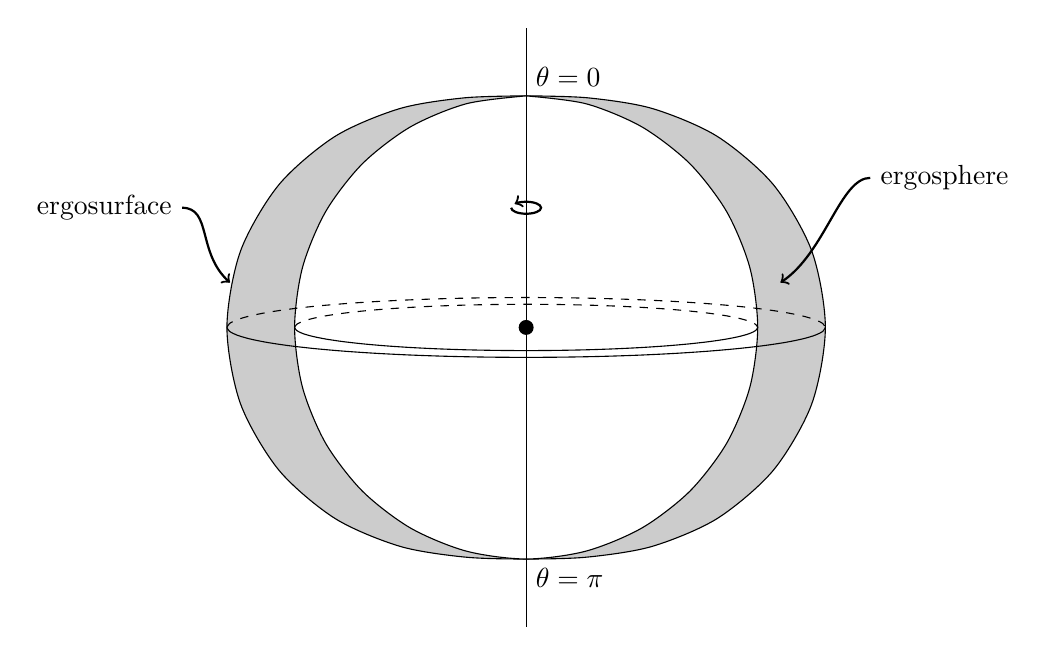
\begin{tikzpicture}[scale=1.9]
        \begin{scope}[rotate=90]
            \draw[domain=0:360,smooth,variable=\x,fill=black!20] plot({(1 + sqrt(1-0.7*cos(\x)*cos(\x)))*cos(\x)},{(1 + sqrt(1-0.7*cos(\x)*cos(\x)))*sin(\x)});
            \draw[domain=0:360,smooth,variable=\x,fill=white] plot({(1 + sqrt(1-0.7))*cos(\x)},{(1 + sqrt(1-0.7))*sin(\x)});
            \draw[domain=90:270,smooth,variable=\x] plot({0.1*(1 + sqrt(1-0.7))*cos(\x)},{(1 + sqrt(1-0.7))*sin(\x)});
            \draw[domain=90:-90,smooth,variable=\x,dashed] plot({0.1*(1 + sqrt(1-0.7))*cos(\x)},{(1 + sqrt(1-0.7))*sin(\x)});
            \draw[domain=90:270,smooth,variable=\x] plot({0.1*2*cos(\x)},{2*sin(\x)});
            \draw[domain=90:-90,smooth,variable=\x,dashed] plot({0.1*2*cos(\x)},{2*sin(\x)});
        \end{scope}
        \fill (0,0) circle (0.05);
        \draw (0,2) -- (0,-2);
        \node[above right] at (0,{1+sqrt(0.3)}) {\(\theta=0\)};
        \node[below right] at (0,{-1-sqrt(0.3)}) {\(\theta=\pi\)};
        \draw[->,thick,yscale=0.4] (-0.1,2) arc (180:500:0.1);

        \draw[<-,thick] (-1.98,0.3) .. controls (-2.2,0.5) and (-2.1,0.8) .. (-2.3,0.8) node[left] {ergosurface};
        \draw[<-,thick] (1.7,0.3) .. controls (2,0.5) and (2.1,1) .. (2.3,1) node[right] {ergosphere};
    \end{tikzpicture}
\end{figure}
Note that stationary observers follow timelike geodesics parallel to \(k\), and these can't exist in the ergosphere.

Consider now a particle with 4-momentum \(P^a = \mu u^a\), where \(\mu\) is the particle's rest mass. Then the energy of the particle with respect to an observer at infinity is given by \(E=-k\vdot P\). Suppose the particle decays inside the ergoregion into two particles with momenta \(P_1\), \(P_2\) respectively.
\begin{figure}[H]
    \centering
    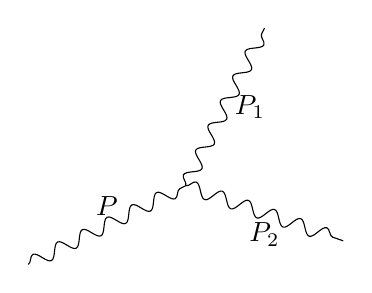
\begin{tikzpicture}
        \draw[decorate,decoration=snake] (0,0) -- (2,1) node[midway,above] {\(P\)};
        \draw[decorate,decoration=snake] (2,1) -- (3,3) node[midway,right] {\(P_1\)};
        \draw[decorate,decoration=snake] (2,1) -- (4,0.3) node[midway,below] {\(P_2\)};
    \end{tikzpicture}
\end{figure}
We have \(E = E_1 + E_2\) where \(E_i=-k\vdot P_i\). Since \(k\) is spacelike, we can have \(E_1<0\). Then \(E_2=E+|E_1|>E\). Particle 1 must fall into the black hole, but particle 2 can escape to infinity. Hence a particle leaves the ergoregion with more energy than when it entered -- this is the \emph{Penrose process}. Since \(E_1<0\), the mass of the black hole decreases.

There is a bound on the amount of energy that can be extracted. Since \(P\) and \(\xi\) are both causal, we have \(-P\vdot\xi\ge0\), so \(-P\vdot(k+\Omega_H m)\ge 0\). Thus \(E-\Omega_HL\ge0\), where \(L=m\vdot P\) is the conserved angular momentum, so \(L\le E/\Omega_H\). After the black hole settles, we have \(\delta M=E\) and \(\delta J = L\), so
\begin{equation}
    \delta J \le \frac{\delta M}{\Omega_H} = \frac{2M(M^2+\sqrt{M^4-J^2})}{J}\delta M.
\end{equation}
It can be shown that this is equivalent to \(\delta M_{\text{irr}} = 0\), where \(M_{\text{irr}} = \left[\frac{1}{2}\left(M^2+\sqrt{M^4+J^2}\right)\right]^{\frac{1}{2}}\) is the ``irreducible mass''. We have
\begin{equation}
    M^2 = M_{\text{irr}}^2 + \frac{J^2}{4M_{\text{irr}}^2} \ge M_{\text{irr}}^2 \ge \text{initial } M_{\text{irr}}^2,
\end{equation}
so the mass can not decrease below the RHS.

It can be shown that \(A=16\pi M_{\text{irr}}^2\) is the area of the event horizon (i.e.\ the area of the intersection of \(\mathcal{H}^+\) with a partial Cauchy surface), so \(\delta A \ge0\) (this is a special case of the second law of black hole mechanics).

\section{Mass, Charge, and Angular Momentum}
\subsection{Charges in curved spacetime}
Consdier a general orientable manifold \((\mathcal{M},g)\) of \(n\) dimensions. We have the volume form \(\epsilon\), satisfying
\begin{equation}
    \epsilon^{a_1\dots a_p c_{p+1} \dots c_n}\epsilon_{b_1\dots b_p c_{p+1} \dots c_n}
    = \pm p!(n-p)! \delta^{a_1}_{[b_1} \dots \delta^{a_p}_{b_p]},
\end{equation}
where \(+\) corresponds to a Riemannian signature, and \(-\) corresponds to a Lorentzian signature.
\begin{defn}
    The \emph{Hodge dual} of a \(p\)-form \(X\) is an \((n-p)\)-form \(\star X\) defined by
    \begin{equation}
        (\star X)_{a_1\dots a_{n-p}} = \frac{1}{p!}\epsilon_{a_1\dots a_{n-p} b_1\dots b_p} X^{b_1\dots b_p}.
    \end{equation}
\end{defn}
It is simple to see that \(\star(\star X) = \pm (-)^{p(n-p)}X\). We also have 
\begin{equation}
    (\star \dd{\star X})_{a_1\dots a_{p-1}} = \pm (-)^{p(n-p)} \nabla^b X_{a_1\dots a_{p-1} b}.
\end{equation}
In Euclidean 3D space, we have:
\begin{align}
    \Delta f &= \dd{f} \\
    \div X &= \star\dd{\star X} \\
    \curl X &= \star\dd{X}
\end{align}

\lecture{24/02/16}
Recall the Maxwell equations
\begin{equation}
    \nabla^aF_{ab} = -4\pi j_b \qq{and} \nabla_{[a}F_{bc]} = 0,
\end{equation}
where \(j\) is the current density 4-vector. In terms of forms we have
\begin{equation}
    \dd{\star F} = -4\pi \star j \qq{and} \dd{F} = 0.
\end{equation}

\begin{defn}
    Let \(\Sigma\) be a spacelike hypersurface. The electric charge \(Q\) on \(\Sigma\) is given by
    \begin{equation}
        Q = -\int_\Sigma \star j = \frac{1}{4\pi}\int_\sigma \dd{\star F} = \frac{1}{4\pi} \int_{\partial\Sigma}\star F.
    \end{equation}
\end{defn}

\begin{eg}
    Consider Minkowski space with spherical coordinates \((t,r,\theta,\phi)\), with orientation given by the volume form \(\epsilon = r^2\sin\theta \dd{t}\wedge\dd{r}\wedge\dd{\theta}\wedge\dd{\phi}\). Let \(\Sigma=\{t=0\}\), with orientation \(\dd{r}\wedge\dd{\theta}\wedge\dd{\phi}\), and \(\Sigma_R = \{t=0,r\le R\}\) with the same orientation. We have \(\partial \sigma_R = \{t=0,r=R\}\) with orientation \(\dd{\theta}\wedge\dd{\phi}\). Consider \(A=-\frac{q}{r}\dd{t}\). We have \(F=\dd{A} = -\frac{q}{r^2}\dd{t}\wedge\dd{r}\). Thus \((\star F)_{\theta\phi} = r^2\sin^2\theta F^{tr} = q\sin\theta\), so
    \begin{equation}
        Q(\Sigma_R) = \frac{1}{4\pi}\int_{S^2_R}\star F = \frac{1}{4\pi}\dd{\theta}\dd{\phi} q\sin\theta = q.
    \end{equation}
\end{eg}

\begin{defn}
    Let \((\Sigma, h_{ab}, K_{ab})\) be an asymptotically flat end, \(S_r^2 = \{x^ix^i=r^2\}\). Then the \emph{electric charge} Q and \emph{magnetic charge} P of the spacetime are given by
    \begin{align}
        Q &= \frac{1}{4\pi} \lim_{r\to\infty} \int_{S_r^2} \star F \\
        P &= \frac{1}{4\pi} \lim_{r\to\infty} \int_{S_r^2} F
    \end{align}
\end{defn}
Exercise: show this agrees with \(Q\) and \(P\) in the Kerr-Newman solution.

\subsection{Komar integrals}
Let \((\mathcal{M},g)\) be a stationary spacetime. There exists a conserved energy-momentum current \(J_a = -T_{ab}k^b\), \(\dd{\star j} = 0\). Hence we can define the total energy of matter on a spacelike hypersurface \(\Sigma\) as
\begin{equation}
    E[\Sigma] = -\int_\Sigma \star J.
\end{equation}
This quantity is conserved. Suppose \(\Sigma\) and \(\Sigma'\) bound a region \(R\) of spacetime.
\begin{figure}[H]
    \centering
    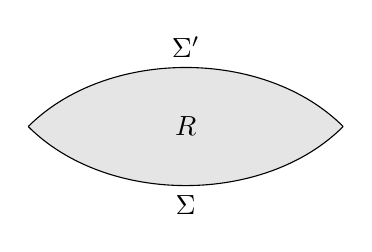
\begin{tikzpicture}
        \fill[black!10] (2,0) .. controls (1,1) and (-1,1) .. (-2,0)
                              .. controls (-1,-1) and (1,-1) .. (2,0);

        \draw (2,0) .. controls (1,1) and (-1,1) .. (-2,0) node[midway,above] {\(\Sigma'\)};
        \draw (2,0) .. controls (1,-1) and (-1,-1) .. (-2,0) node[midway,below] {\(\Sigma\)};
        \node at (0,0) {\(R\)};
    \end{tikzpicture}
\end{figure}
Then we have
\begin{equation}
    E[\Sigma']-E[\Sigma] = - \int_{\partial R} \star J = -\int_R \dd{\star J} = 0.
\end{equation}

\begin{lemma}
    A KVF \(k^a\) obeys \(\nabla_a\nabla_bk^c = R\indices{^c_{bad}}k^d\).
\end{lemma}

Hence we have
\begin{align}
    (\star\dd{\star\dd{k}})_c &= -\nabla^b(\dd{k})_{cb} \\
                              &= -\nabla^b(\nabla_ck_b-\nabla_bk_c) \\
                              &= 2\nabla^b\nabla_bk_c \\
                              &= -2R_{cd} k^d \\
                              &= 8\pi J'_c,
\end{align}
where \(J'_a = -2\left(T_{ab} - \frac{1}{2} T g_{ab}\right) k^b\). Thus \(\dd{\star\dd{k}} = 8\pi \star J\), and
\begin{equation}
    -\int_\Sigma\star J' = -\frac{1}{8\pi}\int_\Sigma \dd{\star\dd{k}} = -\frac{1}{8\pi}\int_{\partial\Sigma} \star \dd{k}.
    \label{emperhaps}
    \tag{\(*\)}
\end{equation}
Exercise: consider a static, spherically symmetric perfect fluid star, and let \(\Sigma = \{t=\text{constant},r\le r_0\}\) where \(r_0 > R = \text{star radius}\). Show that the RHS of \eqref{emperhaps} is the parameter \(M\) in the Schwarzschild solution. Show that the LHS of \eqref{emperhaps} is the total energy of matter in the star in the Newtonian limit (\(p \ll \rho, |\Phi| \ll 1, |\Psi| \ll 1\)).

\begin{defn}
    Let \((\Sigma, h_{ab}, K_{ab})\) be an asymptotically flat end in a stationary spacetime. The \emph{Komar mass} is
    \begin{equation}
        M_{\text{Komar}} = -\frac{1}{8\pi}\lim_{r\to\infty}\int_{S_r^2}\star\dd{k}.
    \end{equation}
    If we have axisymmetry, then the \emph{Komar angular momentum} is
    \begin{equation}
        J_{\text{Komar}} = \frac{1}{16\pi}\lim_{r\to\infty}\int_{S_r^2}\star\dd{m}.
    \end{equation}
\end{defn}
It can be shown that for the Kerr-Newman solution, we have \(M_{\text{Komar}} = M\) and \(J_{\text{Komar}} = J\).

\subsection{Hamiltonian formulation of GR}
Set \(16\pi G=1\), and assume global hyperbolicity, so that we can write
\begin{equation}
    \dd{s}^2 = -N^2\dd{t} + h_{ij}(\dd{x}^i + N^i\dd{t})(\dd{x}^j + N^j\dd{t}).
\end{equation}
We have the following action in the 3+1 formulation:
\begin{equation}
    S = \int\dd{t}\dd[3]{x} \mathcal{L} = \int \dd{t}\dd[3]{x}N\sqrt{H}\left({}^{(3)}R - K_{ij}K^{ij} + K^2\right)
\end{equation}
\({}^{(3)}R\) is the Ricci scalar of \(h_{ij}\), and \(K\) is the trace of \(K_{ij}\) the extrinsic curvature associated with \(t=0\), given by
\begin{equation}
    K_{ij} = \frac{1}{2N}(\dot{h}_{ij} - D_iN_j-D_jN_i),
\end{equation}
where \(D\) is the covariant derivative with respect to \(h_{ij}\). \(ijk\) indices are raised and lowered with \(h\).

Note that \(S\) is a function of \(N\), \(N^i\) and \(h_{ij}\) only -- it is independent of \(\partial_t N\) and \(\partial_t N^i\). If we vary \(N\) we obtain the Hamiltonian constraint, and if we vary \(N^i\) we obtain the momentum constraint.

The momentum conjugate to \(h\) is given by
\begin{equation}
    \pi^{ij} = \fdv{S}{\dot{h}_{ij}} = \sqrt{h}(K^{ij}-Kh^{ij}).
\end{equation}
The Hamiltonian is thus
\begin{equation}
    H = \int \dd[3]{x}(\pi^{ij}\dot{h}_{ij} - \mathcal{L}) = \int \dd[3]{x} \sqrt{h}[N\mathcal{H} + N^i\mathcal{H}_i],
\end{equation}
where
\begin{equation}
    \mathcal{H} = -{}^{(3)}R + h^{-1}\pi^{ij}\pi_{ij} - \frac{1}{2}h^{-1}\pi^2, \qquad \pi=h^{ij}\pi_{ij}
\end{equation}
and
\begin{equation}
    \mathcal{H}_i = -2h_{ik}D_j\left(h^{-\frac{1}{2}}\pi^{jk}\right).
\end{equation}
\(N\) and \(N_i\) play the role of Lagrange multipliers, so on a solution \(\mathcal{H}=\mathcal{H}_i=0\). The equations of motion are 
\begin{equation}
    \dot{h}_{ij} = \fdv{H}{\pi^{ij}},\quad \dot{\pi}_{ij} = - \fdv{H}{h^{ij}}.
\end{equation}
Using this Hamiltonian we'd like to be able to define an energy, but there is a problem: on any solution, \(H=0\).

\lecture{26/02/16}
To fix this, we will need to introduce a boundary term into the Hamiltonian. We assume that the \(t = \text{constant}\) is an asymptotically flat end, so we can write:
\begin{align}
    h_{ij} &= \delta_{ij} + O\left(\frac{1}{r}\right) & \pi_{ij} = O\left(\frac{1}{r^2}\right) \\
    \delta h_{ij} &= O\left(\frac{1}{r}\right) & \delta\pi_{ij} = O\left(\frac{1}{r^2}\right)
\end{align}
Comparing with the expression for the metric in terms of \(N\) and \(N^i\), we see that we must have \(N=1+O\left(\frac{1}{r}\right)\) and \(N^i\to0\) as \(r\to \infty\). Under these assumptions, we find that the variation of the Hamiltonian takes the form
\begin{equation}
    \delta H = \int\dd[3]{x}(\dots)\delta h_{ij} - \underbrace{\delta E_{\text{ADM}}}_{\mathclap{\text{surface term}}}
\end{equation}
where
\begin{equation}
    E_{\text{ADM}} = \lim_{r\to\infty} \int_{S^2_r} \dd{A} n_i (\partial_j h_{ij} - \partial_i h_{jj}).
\end{equation}
\(\dd{A}\) is the area element on \(S^2_r\) and \(n_i\) is the outward unit normal to \(S^2_r\). We can thus replace the Hamiltonian \(H\) by \(H' = H + E_{\text{ADM}}\). Since they differ by a surface term, the equations of motion give the same result, but now we have no runaway boundary terms when varying \(h_{ij}\). Thus \(H'\) is the true Hamiltonian of GR.

\subsection{ADM energy}
Since \(H = 0\) on a solution, the energy of the spacetime must be given by \(E_{\text{ADM}}\). Return to \(G=1\) units and we have:
\begin{defn}
    The \emph{Arnowitt-Deser-Misner energy} of an asymptoticall flat end is
    \begin{equation}
        E_{\text{ADM}} = \frac{1}{16\pi}\lim_{r\to\infty}\int_{S^2_r}\dd{A}n_i(\partial_j h_{ij} - \partial_i h_{jj}).
    \end{equation}
\end{defn}

In a stationary spacetime, if the constant \(t\) surface is orthogonal to \(k^a\) as \(r\to\infty\), then it can be shown that \(E_{\text{ADM}} = M_{\text{Komar}}\).

Similarly, we have:
\begin{defn}
    The \emph{ADM 3-momentum} of an asymptotically flat end is
    \begin{equation}
        P_i = \frac{1}{8\pi}\lim_{r\to\infty}\int_{S^2_r} \dd{A}(K_{ij}n_j-Kn_i).
    \end{equation}
\end{defn}

\begin{theorem}
    Let \((\Sigma, h_{ab}, K_{ab})\) be a geodesically complete asymptotically flat end obeying the DEC. Then \(E_{\text{ADM}} \ge \sqrt{P_iP_i}\), with equality iff \((\Sigma,h_{ab},K_{ab})\) is a surface in Minkowski spacetime.
\end{theorem}

\begin{defn}
    The \emph{ADM mass} of an asymptotically flat end is
    \begin{equation}
        M_{\text{ADM}} = \sqrt{E_{\text{ADM}} - P_iP_i}.
    \end{equation}
\end{defn}

\section{Black Hole Mechanics}
\subsection{Killing horizons and surface gravity}
\begin{defn}
    A null hypersurface \(\mathcal{N}\) is a \emph{Killing horizon} if there exists a KVF \(\xi^a\) defined in a neighbourhood of \(\mathcal{N}\) such that \(\xi^a\) is normal to \(\mathcal{N}\).
\end{defn}
\begin{theorem}
    In a stationary, analytic, asymptotically flat, vacuum black hole solution, \(\mathcal{H}^+\) is a Killing horizon.
\end{theorem}
For example, in Kerr \(\{r=r_+\}\) is a Killing horizon with normal KVF \(\xi^a = k^a+\Omega_H m^a\).

It can be shown that if \(\xi^a\) is not parallel to \(k^a\), then \((\mathcal{M},g)\) is stationary and axisymmetric. We normalise so that \(k^2\to-1\) at \(\infty\), and write \(\xi^a = k^a + \Omega_H m^a\), where \(m^a\) is the generator of axisymmetry. Since \(\left.\xi\vdot\xi\right|_{\mathcal{N}} = 0\), we have that \(\dd{\xi^a\xi_a}\) is orthogonal to \(\mathcal{N}\). Therefore there exists a \(\kappa\) such that
\begin{equation}
    \left.\nabla_a(\xi_b\xi^b)\right|_{\mathcal{N}} = -2\kappa\xi_a.
\end{equation}
\(\kappa\) is called the \emph{surface gravity} of \(\mathcal{N}\). Since \(\xi_a\) is a KVF, we have \(\nabla_a(\xi_b\xi^b) = 2\xi_b\nabla_a\xi^b = -2\xi^b\nabla_b\xi_a\), so we can write the above as
\begin{equation}
    \left.\xi^b\nabla_b\xi^a\right|_{\mathcal{N}} = \kappa\xi_a.
\end{equation}
Let \(n^a\) be tangent to the affinely parametrised generators of \(\mathcal{N}\). Then \(\xi^a = fn^a\) on \(\mathcal{N}\) and we have
\begin{equation}
    \xi^b\nabla_b\xi^a = fn^b\nabla_b(fn^a) = f^2\underbrace{n^b\nabla n^a}_{=0} + f n^a n^b\nabla_b f = \xi^a\xi^b\partial_b\log|f|,
\end{equation}
so \(\kappa = \xi^a\partial_a\log|f|\).
\begin{eg}
    Consider a Reissner-Nordstrom black hole.
    \begin{equation}
        \dd{s}^2 = -\frac{\Delta}{r^2} \dd{v}^2 + 2\dd{v}\dd{r} + r^2\dd{\Omega}^2
    \end{equation}
    where \(\Delta = (r-r_+)(r-r_-)\), \(r_\pm = M \pm \sqrt{M^2-e^2}\). We have \(k=\pdv{v}\) and \(\left.k_a\right|_{r=r_\pm}=(\dd{r})_a\). Thus \(k_a\) is orthogonal to the null hypersurfaces \(r=r_\pm\), so these are Killing horizons. We have
    \begin{align}
        \dd{(k^bk_b)} &= \dd{\left(-\frac{\nabla}{r^2}\right)} \\
                      &= \left(-\frac{\nabla'}{r^2} + \frac{2\nabla}{r^3}\right)\dd{r} \\
        \implies \left.\dd{(k^bk_b)}\right|_{r=r_\pm} &= - \left(\frac{r_\pm-r_\mp}{r_\pm^2}\right)k_a
    \end{align}
    and therefore the surface gravities at \(r_\pm\) are \(\kappa = \frac{r_\pm-r_\mp}{2r_\pm^2}\).
    
    If we set \(e=0\) we obtain Schwarzschild with \(r_+ = 2M\), \(r_- = 0\) and \(\kappa = \frac{1}{4M}\).

    If we set \(e=M\), we obtain extreme RN with \(r_+ = r_- = M\) and \(\kappa = 0\).
\end{eg}

Exercise: in the Kruskal spacetime, show that \(\mathcal{H}^\pm\) are Killing horizons \(\mathcal{N}^\pm\) of \(k^a\) with surface gravities \(\pm\frac{1}{4M}\). This is an example of a \emph{bifurcate} Killing horizon. \(\mathcal{N}^\pm\) are both Killing with respect to \(\xi^a\), and they are orthogonal, so on \(B = \mathcal{N}^+\cap\mathcal{N}^-\), \(\xi\) must vanish. Any \(X^a\) tangent to \(B\) must also be tangent to both of \(\mathcal{N}^\pm\), so \(X^a\) is spacelike, and \(B\) is a spacelike 2-surface.

\subsection{Interpretation of the surface gravity}
The main reason that \(\kappa\) is important is because the Hawking temperature (see later) is \(\frac{\hbar\kappa}{2\pi}\). However there is another interpretation. In a static, asymptotically flat spacetime, \(\kappa\) is the force per unit rest mass at infinity needed to hold a particle at rest on the horizon.

\subsection{Zeroth law of BH mechanics}
\lecture{29/02/16}

\begin{lemma}
    Consider a null geodesic congruence containing the generators of a Killing horizon \(\mathcal{N}\). Then \(\theta = \hat{\sigma} = \hat{\omega} = 0\) on \(\mathcal{N}\).
\end{lemma}
\begin{proof}
    We already have \(\hat{\omega}=0\) since the generators are hypersurface orthogonal.

    Let \(\xi^a\) be a KVF normal to \(\mathcal{N}\), and \(U^a\) be tangent to the affinely parameterised generators of \(\mathcal{N}\). We can write \(\xi^a = hU^a\) on \(\mathcal{N}\). Thus \(U^a = h^{-1}\xi^a + fV^a\) for some \(V^a\) and \(f\) that vanishes on \(\mathcal{M}\). Then we have
    \begin{equation}
        B_{ab} = \nabla_bU_a = (\partial_bh^{-1})\xi_a + h^{-1}\nabla_b\xi_a + (\partial_bf)V_a + f\nabla_bV_a.
    \end{equation}
    Evaluating on \(\mathcal{N}\), using Killing's equation, and symmetrising, we obtain
    \begin{equation}
        \left.B_{(ab)}\right|_\mathcal{N} = \left(\xi_{(a}\partial_{b)}h^{-1} + V_{(a)}\partial_{b)}f\right)_\mathcal{N}.
    \end{equation}
    \(\xi_a,\partial_af\) are parallel to \(U_a\) on \(\mathcal{N}\), so after projecting onto \(T_\perp\), we get
    \begin{equation}
        \left.\hat{B}_{(ab)}\right|_\mathcal{N} = 0,
    \end{equation}
    so \(\theta\) and \(\hat{\sigma}\) vanish.
\end{proof}

\begin{theorem}[zeroth law]
    \(\kappa\) is constant on the future event horizon of a stationary black hole spacetime obeying the dominant energy condition.
\end{theorem}
\begin{proof}
    We have that \(\mathcal{H}^+\) is a Killing horizon with respect to some KVF \(\xi^a\). From the above lemma, \(\theta=\hat{\omega}=\hat{\sigma}=0\) along generators of \(\mathcal{H}^+\), so by Raychaudhuri's equation we have
    \begin{equation}
        0 = \left.R_{ab}\xi^a\xi^b\right|_{\mathcal{H}^+} = \left.8\pi T_{ab}\xi^a\xi^b\right|_{\mathcal{H}^+},
    \end{equation}
    using the fact that \(\xi\) is null in the second equality. Thus \(\left.J\vdot\xi\right|_{\mathcal{H}^+}=0\) where \(J_a=-T_{ab}\xi^b\). Since \(\xi^a\) is future-directed and causal, the DEC implies that so is \(J^a\) (unless \(J^a=0\)). Hence we must have \(J^a\) parallel to \(\xi^a\) on \(\mathcal{H}^+\). Thus
    \begin{equation}
        0 = \left.\xi_{[a}J_{b]}\right|_{\mathcal{H}^+} = -\left.\xi_{[a}T_{b]c}\xi^c\right|_{\mathcal{H}^+} = -\frac{1}{8\pi}\left.\xi_{[a}R_{b]c}\xi^c\right|_{\mathcal{H}^+}.
    \end{equation}
    It can be shown that this implies
    \begin{equation}
        0 = \frac{1}{8\pi}\xi_{[a}\partial_{b]}\kappa,
    \end{equation}
    so \(\partial_a{\kappa}\) is proportional to \(\xi_a\), so \(t\vdot\partial\kappa=0\) for any vector field \(t^a\) tangent to \(\mathcal{H}^+\), and therefore \(\kappa\) is constant on \(\mathcal{H}^+\) (assuming \(\mathcal{H}^+\) is connected).
\end{proof}

\subsection{First law of BH mechanics}
For a Kerr black hole, if we make small perturbations to \(M\) and \(a\), then it is possible to show that
\begin{equation}
    \frac{\kappa}{8\pi}\delta A = \delta M - \Omega_H \delta J.
    \tag{\(*\)}
    \label{firstlaw}
\end{equation}
In fact this holds under more more general perturbations. Take a spatial hypersurface \(\Sigma\) with \(\Sigma \perp k^a\) near to \(i^0\). Make a small perturbation to the initial data on \(\Sigma\), satisfying the constraint equations to \(1^{\text{st}}\) order. Then \eqref{firstlaw} is satisfied, where \(\delta A\) is the change in area of the bifurcation surface \(A\), \(\delta M\) is the change in ADM mass, \(\partial J\) is the change in ADM angular momentum (defined analogously to ADM mass). (For Einstein-Maxwell theory, we get an extra term \(\Phi_H \delta Q\) on the RHS, where \(\Phi_H\) is the potential difference between the eveny horizon and infinity.)

There is another version of this law. Suppose we start with a Kerr spacetime and add an energy-momentum tensor \(T_{ab}=O(\epsilon)\). Then we can define \(J^c = -T\indices{^a_b}k^b\) and \(L^a = T\indices{^a_b}m^b\). We find that \(\nabla_a J^a\) and \(\nabla_a L^a\) are \(O(\epsilon^2)\), so these are conserved to first order.

Let \(\mathcal{N}\) be the portion of \(\mathcal{H}^+\) to the future of \(B\), and consider the case where some matter crosses \(\mathcal{N}\). The energy crossing \(\mathcal{N}\) is
\begin{equation}
    \delta M = -\int_{\mathcal{N}} *J
\end{equation}
and the angular momentum is
\begin{equation}
    \delta J = -\int_{\mathcal{N}} *J.
\end{equation}
Pick coordinates \((y_1,y_2)\) on \(B\), and let \(\lambda\) be the affine parameter distance along generators of \(\mathcal{N}\) from \(B\) and \(r\) the affine parameter along null geodesics orthogonal to \(\mathcal{N}\). The metric takes the form \(\left.\dd{s}^2\right|_{\mathcal{N}} = 2\dd{r}\dd{\lambda}+h_{ij}\dd{y^i}\dd{y^j}\) and hence the volume form is \(\left.\eta\right|_{\mathcal{N}} = \sqrt{h}\dd{\lambda}\wedge\dd{r}\wedge\dd{y^1}\wedge\dd{y^2}\). The orientation of \(\mathcal{N}\) to use in evaluating the integrals is the one used in Stokes' theorem, viewing \(\mathcal{N}\) as the boundary of the region \(r>0\). This is \(\dd{\lambda}\wedge\dd{y^1}\wedge\dd{y^2}\). On \(\mathcal{N}\) we then have
\begin{equation}
    (*J)_{\lambda 12} = \sqrt{h}J^r = \sqrt{h}J_\lambda = \sqrt{h}U\vdot J
\end{equation}
where \(U = \pdv{\lambda}\). Hence
\begin{equation}
    \delta M = -\int_{\mathcal{N}}\dd{\lambda}\dd[2]{y} \sqrt{h}U\vdot J
\end{equation}
and
\begin{equation}
    \delta J = -\int_{\mathcal{N}}\dd{\lambda}\dd[2]{y} \sqrt{h}U\vdot L.
\end{equation}
To order \(\epsilon\), we can replace \(h\) by \(g\) in these expressions. Thus we can use the fact that \(N\) is a Killing horizon with KVF \(\xi^a=k^a+\Omega_H m^a\). Hence \(\left.\xi\right|_{\mathcal{N}}=fU^a\), and
\begin{equation}
    \xi\vdot\dd{\log|f|}=\kappa \implies U\vdot\dd{f}=\kappa \implies \pdv{f}{\lambda}=\kappa. 
\end{equation}
Thus \(f=\kappa\lambda + f_0(y)\). Since \(\left.\xi^a\right|_B=0\), we have \(f_0=0\), so \(\left.xi^a\right|_{\mathcal{N}}=\kappa\lambda U^a\). Hence
\begin{align}
    \partial M &= \int_{\mathcal{N}} \dd{\lambda}\dd[2]{y}\sqrt{h}T_{ab}U^ak^b \\
               &= \int_{\mathcal{N}} \dd{\lambda}\dd[2]{y}\sqrt{h}T_{ab}U^a(\xi^b-\Omega_H m^b) \\
               &= 
    \kappa\int_{\mathcal{N}} \dd{\lambda}\dd[2]{y}\lambda\sqrt{h}\underbrace{T_{ab}U^aU^b}_{\mathclap{=\frac{1}{8\pi}R_{ab}U^aU^b}}
    - \Omega_H\underbrace{\int_{\mathcal{N}} \dd{\lambda}\dd[2]{y}\sqrt{h}T_{ab}U^a m^b}_{=-\delta J}
\end{align}
\begin{equation}
    \implies \delta M - \Omega_H \delta J = \frac{\kappa}{8\pi} \int_{\mathcal{N}}\dd{\lambda}\dd[2]{y}\sqrt{h}\lambda R_{ab}U^aU^b.
\end{equation}
Using Raychaudhuri's equation
\begin{equation}
    \dv{\theta}{\lambda} = \underbrace{\dots}_{O(\epsilon^2)} - R_{ab}U^aU^b
\end{equation}
we have
\begin{align}
    \delta M-\Omega_H\delta J &= - \frac{\kappa}{8\pi} \int\dd[2]{y}\int_0^\infty\dd{\lambda}\sqrt{h}\lambda\dv{\theta}{\lambda}\\
                              &= - \frac{\kappa}{8\pi} \int\dd[2]{y}\left\{ [\sqrt{h}\lambda\theta]^\infty_0 - \int^\infty_0\dd{\lambda}\left(\sqrt{h}+\lambda\dv{\sqrt{h}}{\lambda}\right)\theta\right\}
\end{align}
Recall that \(\dv{\sqrt{h}}{\lambda} = \theta\sqrt{h} = O(\epsilon)\), so the \(\lambda \dv{\sqrt{h}}{\lambda}\theta\) term is \(O(\epsilon^2)\) and can be ignored. We assume that the spacetime settles down to some stationary final state, so that \(\sqrt{h}\to\) some finite limit as \(\lambda \to \infty\). Then 
\begin{equation}
    \int^\infty_0\sqrt{h}\theta\dd{\lambda} = \int_0^\infty \dv{\sqrt{h}}{\lambda} \dd{\lambda} = [\sqrt{h}]_0^\infty = \delta\sqrt{h}
\end{equation}
is finite. Thus \(\theta\) must be \(o(1/\lambda)\), so the boundary term \([\sqrt{h}\lambda\theta]^\infty_0=0\) also. Finally we have
\begin{equation}
    \delta M - \Omega_H \delta J = \frac{\kappa}{8\pi}\int_B\delta\sqrt{H}\dd[2]{y} = \frac{\kappa}{8\pi} \delta A,
\end{equation}
where \(\delta A\) is the change in the area of the horizon between early and late times.

\subsection{Second law of BH mechanics}
\lecture{02/03/16}
\begin{theorem}[second law]
    Let \((\mathcal{M},g)\) be a strongly asymptotically predictable spacetime that obeys Einstein's equations and the NEC. Let \(U\in\mathcal{M}\) be a globally hyperbolic region with \(\overline{J^-(\scri^+)}\subset U\), \(\Sigma_1,\Sigma_2\) be spacelike Cauchy surfaces for \(U\) such that \(\Sigma_2 \subset J^+(\Sigma_1)\), and \(H_i = \Sigma_i \cap \mathcal{H}^+\). Then \(\operatorname{area}(H_2)\ge\operatorname{area}(H_1)\).
\end{theorem}

\begin{figure}[H]
    \centering
    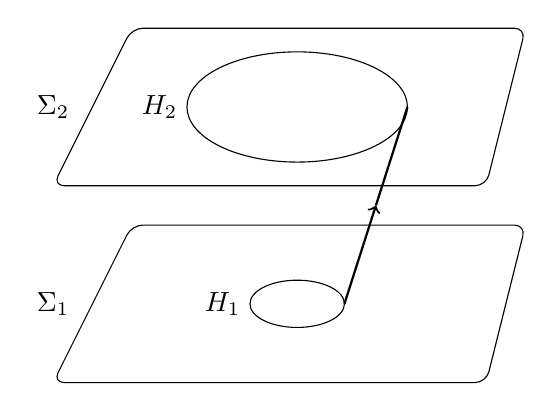
\begin{tikzpicture}
            \draw[rounded corners] (0,0) -- (1,2) -- (6,2) -- (5.5,0) -- cycle;
            \draw[rounded corners] (0,2.5) -- (1,4.5) -- (6,4.5) -- (5.5,2.5) -- cycle;

            \node at (0,1) {\(\Sigma_1\)};
            \node at (0,3.5) {\(\Sigma_2\)};

            \draw (3.1,1) ellipse (0.6 and 0.3);

            \draw (3.1,3.5) ellipse (1.4 and 0.7);

            \draw[thick,->] (3.7,1) -- (4.1,2.25);
            \draw[thick] (4.1,2.25) -- (4.5,3.5);
        
            \node[left] at (2.5,1) {\(H_1\)};
            \node[left] at (1.7,3.5) {\(H_2\)};
    \end{tikzpicture}
\end{figure}
\begin{proof}
    Assume that the inextendible generators of \(\mathcal{H}^+\) are future-complete (we say \(\mathcal{H}\) is \emph{non-singular}. Suppose \(\theta < 0\) at some \(p \in \mathcal{H}^+\). By continuity, \(\theta < 0\) at some \(q \in \mathcal{H}^+\) in the near future of \(p\) along a geodesic \(\gamma\), and therefore there is a point \(r\) conjugate to \(p\) along \(\gamma\). Therefore we can deform \(\gamma\) into a timelike curve from \(p\) to \(r\), but \(\mathcal{H}^+\) is achronal, so this is a contradiction, and thus \(\theta \ge 0\) on \(\mathcal{H}^+\).

    Let \(p\in H_1\). The generator of \(\mathcal{H}^+\) through \(p\) cannot leave \(\mathcal{H}^+\), since generators don't have future endpoints, so it must intersect \(H_2\) (as \(\Sigma_2\) is a Cauchy surface). This defines a map \(\phi:H_1\to H_2\). We have \(\operatorname{area}(H_2)>\operatorname{area}(\phi(H_1))\) since \(\phi(H_1)\subset H_2\). Since \(\theta \ge 0\), we have \(\operatorname{area}(\phi(H_1))\ge\operatorname{area}(H_1)\).
\end{proof}

\begin{eg}
    In the spherical collapse of a star into a black hole, the radius of \(\mathcal{H}^+\) can only increase.
\end{eg}
\begin{eg}
    Consider the merger of 2 black holes of areas \(A_1\) and \(A_2\) that are initially Schwarzschild and well-seperated, and settle down to a Schwarzschild final state with area \(A_3\)

    The second law tells us that \(A_3 \ge A_1 + A_2\). In particular this means
    \begin{equation}
        16\pi M_3^2 \ge 16\pi(M_1^2 + M_2^2)
    \end{equation}
    and so we have a lower bound on the mass of the final black hole \(M_3 \ge \sqrt{M_1^2 + M_2^2}\). The energy radiated in the merger is \(M_1 + M_2 - M_3\), so we have an upper bound on the efficiency of the merger
    \begin{equation}
        \frac{M_1+M_2-M_3}{M_1+M_2} \le 1 - \frac{\sqrt{M_1^2+M_2^2}}{M_1+M_2} \le 1 - \frac{1}{\sqrt{2}}.
    \end{equation}
\end{eg}

Consider initial data \((\Sigma,h_{ab},K_{ab})\) that is asymptotically flat with a trapped surface behind an apparent horizon of area \(A_{\text{app}}\), and let \(E_i\) be the ADM energy of this data. Weak cosmic censorship says this should settle down to a stationary black hole at late time, and the uniqueness theorems say it should be a Kerr black hole; let the mass of this black hole be \(M_f\) and its angular momentum be \(J_f\). By the second law, \(A_{\text{app}} \le A_i\), and we have 
\begin{equation}
    A_i\le A_{\text{Kerr}} = 8\pi \left(M_f^2 + \sqrt{M_f^4-J_f^2}\right) \le 16\pi M_f^2 \le 16\pi E_i^2,
\end{equation}
where the last inequality holds because energy can only be carried away (by gravitational waves) in this process. Hence we have the \emph{Penrose inequality}:
\begin{equation}
    E_i \ge \sqrt{\frac{A_{\text{app}}}{16\pi}}
\end{equation}

\section{QFT in Curved Spacetime}
Consider a black hole in its rest frame i.e.\ with ADM energy \(E=M\). The first law of black hole mechanics
\begin{equation}
    \dd{E} = \frac{\kappa}{8\pi} \dd{A} + \Omega_H\dd{J}
\end{equation}
looks a lot like the first law of thermodynamics
\begin{equation}
    \dd{E} = T\dd{S} + \mu\dd{J}.
\end{equation}
This suggests a correspondence
\begin{equation}
    \begin{array}{rcl}
        \text{thermodynamics} & \leftrightarrow & \text{BH mechanics} \\
        T &\leftrightarrow& \lambda\kappa\\
        S &\leftrightarrow& \frac{A}{8\pi\lambda}\\
        \mu &\leftrightarrow& \Omega_H
    \end{array}
\end{equation}
for some constant \(\lambda\). The zeroth laws say that \(T\) and \(\kappa\) are constant in equilibrium. The second laws say that \(S\) and \(A\) cannot decrease.

This seems to suggest that black holes are thermal objects, but classical general relativity forbids the radiation that we would exect such objects to have. If however we take quantum mechanics into account, we will see that black holes \emph{do} radiate, with temperature \(T_H=\frac{\hbar\kappa}{2\pi}\) (so \(\lambda = \frac{\hbar}{2\pi}\)).

\subsection{Free scalar field}
We assume that the spacetime \((\mathcal{M},g)\) is globally hyperbolic, with metric given by
\begin{equation}
    \dd{s}^2 = -N\dd{t}^2 + h_{ij}(\dd{X}^i+N^i\dd{t})(\dd{X}^j+N^j\dd{t}).
\end{equation}
Let \(\Sigma_t\) denote the Cauchy surfaces given by \(t\) constant, and \(n_a\) be their normal. We have \(n_a = -N(\dd{t})_a\) and \(\sqrt{-g} = N\sqrt{h}\). The action for the free scalar field is
\begin{equation}
    S = \int_\mathcal{M} \dd{T}\dd[3]{x}\sqrt{-g}\left(-\frac{1}{2}g^{ab}\partial_a\phi\partial_b\phi-\frac{1}{2}m^2\phi^2\right).
\end{equation}
Varying \(\phi\) gives the Klein-Gordon equation
\begin{equation}
    g^{ab}\nabla_a\nabla_b\phi - m^2\phi = 0,
\end{equation}
and its conjugate momentum is given by
\begin{align}
    \pi(x) = \fdv{S}{(\partial_t\phi(x))}
    &= -\sqrt{-g}g^{t\mu}\partial_\mu\phi \\
    &= -N\sqrt{h}(\dd{t})_\nu g^{\nu\mu}\partial_\mu\phi \\
    &= \sqrt{h}n^\mu\partial_\mu\phi.
\end{align}
To quantise, we promote \(\phi(x)\) and \(\pi(x)\) to operators and impose the canonical commutation relations
\begin{equation}
    [\phi(t,\vb{x}),\pi(t,\vb{x}')] = i\delta^3(\vb{x}-\vb{x}'),
\end{equation}
\begin{equation}
    [\phi(t,\vb{x}),\phi(t,\vb{x}')] = [\pi(t,\vb{x}),\pi(t,\vb{x}')] = 0.
\end{equation}

In the classical picture we define \(S\) to be the set of complex solutions of the Klein-Gordon equation. Note that these solutions are specified uniquely by \(\phi,\partial\phi\) on \(\Sigma_0\). Let \(\alpha,\beta\in S\). We define a bilinear form on \(S\) by
\begin{equation}
    (\alpha,\beta) = -\int_{\Sigma_0}\dd[3]{x}\sqrt{h}n_aj^a(\alpha,\beta) \qq{where} j(\alpha,\beta) = -i (\overline{\alpha}\dd{\beta}-\beta\dd{\overline{\alpha}}).
\end{equation}
Note that \(\nabla^aj_a=-i(\overline{\alpha}\nabla^2\beta-\beta\nabla^2\overline{\alpha}) = -im^2(\overline{\alpha}\beta-\beta\overline{\alpha}) = 0\), so the integral is independent of the choice of Cauchy surface.

This bilinear form has the following properties:
\begin{itemize}
    \item It is \emph{Hermitian}: \((\alpha,\beta)=\overline{(\beta,\alpha)}\).
    \item It is non-degenerate: \((\alpha,\beta) = 0 \Forall \beta \implies \alpha=0\).
    \item \((\alpha,\beta) = - (\overline{\beta},\overline{\alpha})\).
\end{itemize}
Note that it is not positive definite (as for example the last property above implies \((\alpha,\alpha) = - (\overline{\alpha},\overline{\alpha})\)).

In Minkowski space, \((\cdot,\cdot)\) is positive definite for \(S_p=\{\text{positive frequency solutions}\}\). A basis for \(S_p\), labelled by momentum \(\vb{p}\), is given by
\begin{equation}
    \psi_{\vb{p}} = \frac{1}{(2\pi)^{\frac{3}{2}}(2p^0)^{\frac{1}{2}}}e^{ip\vdot x},
\end{equation}
where \(p^0 = \sqrt{\vb{p}^2+m^2}\). If \(k=\pdv{t}\), then \(\mathcal{L}_k\psi_{\vb{p}}=-ip^0\psi_{\vb{p}}\), so its eigenvalue is negative imaginary, which is what we mean by positive frequency. Similarly, \(\overline{\psi_{\vb{p}}}\) has negative frequency, and we denote the space of these solutions by \(\overline{S_p}\). Note that \(S_p\) and \(\overline{S_p}\) are orthogonal, and we have \(S=S_p\oplus\overline{S_p}\).

In a curved spacetime, there is no a priori concept of positive frequency. We will make a choice of decomposition such that the following holds:
\begin{equation}
    S = \underbrace{S_p}_{\mathclap{\substack{\text{positive frequency}\\(\cdot,\cdot)>0}}}
    \oplus
    \overbrace{\overline{S_p}}^{\mathclap{\substack{\text{negative frequency}\\(\cdot,\cdot)<0}}}
\end{equation}
In a general spacetime there are many ways to do this.

\lecture{04/03/16}
We define positive frequency creation and annihilation operators for a mode \(f\in S_p\) by \(a(f) = (f,\phi)\) and \(\herm{a}(f) = -(\overline{f},\phi)\) (this is consistent because \(\phi=\herm{\phi}\)). For example, in Minkowski space \(f=\psi_{\vb{p}}\) for some \(\vb{p}\), and \(a(f) = a_{\vb{p}}\). When we promote these to operators, the canonical commutation relations imply
\begin{equation}
    [a(f),\herm{a(g)}] = (f,g) \qq{and} [a(f),a(g)]=[\herm{a(f)},\herm{a(g)}] = 0.
\end{equation}

We define a vacuum state \(\ket{0}\) by \(a(f)\ket{0}=0\) for all \(f\in S_p\), normalised so that \(\braket{0}{0}=1\). Given a basis \(\{\psi_i\}\) for \(S_p\), we write \(a_i=a(\psi_i)\). An \(N\)-particle state is then given by
\begin{equation}
    a_{i_1}^\dagger a_{i_2}^\dagger \dots a_{i_N}^\dagger \ket{0}.
\end{equation}
The Hilbert space of the theory is spanned by \(\ket{0}\), 1-particle states, 2-particle states, and so on. This space has positive definite inner product, for example
\begin{align}
    \norm{a^\dagger(f)\ket{0}}^2 &= \mel{0}{a(f)a^\dagger(f)}{0} \\
                                 &= \mel{0}{[a(f),a^\dagger(f)]}{0} \\
                                 &= (f,f)\braket{0}{0} \\
                                 &= (f,f) > 0.
\end{align}

Now suppose we choose a different decomposition \(S = S_p' \oplus \overline{S_p'}\). Let \(f'\in S_p'\) and write \(f' = f + \overline{g}\), where \(f,g\in S_p\). Then \(a(f') = (f,\phi) + (\overline{g},\phi) = a(f)-a(g)^\dagger\), and we have \(a(f')\ket{0}\ne0\), i.e.\ \(\ket{0}\) is not the vacuum with respect to \(S_p'\). Thus we can see that the concept of a particle is ambiguous in general when considering QFT in a curved spacetime.

Consider a stationary spacetime with future-directed timelike KVF \(k^a\). This gives a map \(\mathcal{L}_k:S\to S\) that is antiHermitian with respect to \((\cdot,\cdot)\), so its eigenvalues are imaginary. We write \(\mathcal{L}_ku=-i\omega u\) and define positive frequency by \(\omega>0\), which implies \((u,u)>0\). In this case there \emph{is} a preferred definition of particles, as we can just write \(S_p = \{\text{positive frequency modes}\}\).

\subsection{Bogoliubov transformations}
Let \(\{\psi_i\}\) be an orthonormal basis for \(S_p\), so that
\begin{equation}
    (\psi_i,\psi_j) = \delta_{ij} \qq{and} (\psi_i,\overline{\psi_j})=0,
\end{equation}
and define \(a_i=a(\psi_i)\). We cam decompose any state \(\phi\) in terms of this basis
\begin{equation}
    \phi = \sum_i \left(a_i\psi_i + a_i^\dagger\overline{\psi_i}\right),
\end{equation}
and the commutation relations become
\begin{equation}
    [a_i,a_j]=\delta_{ij},\quad[a_i,a_j]=[a_i^\dagger,a_j^\dagger]=0.
\end{equation}
Now let \(S_p'\) be another choice, with orthonormal basis \(\{\psi_i'\}\). The \emph{Bogoliubov transformation} defines this change of basis by two matrices \(A\) and \(B\):
\begin{align}
    \psi_i' &= \sum_j \left(A_{ij}\psi_j + B_{ij}\overline{\psi_j}\right) \\
    \overline{\psi_j'} &= \sum_j \left(\overline{B_{ij}}\psi_j + \overline{A_{ij}}\overline{\psi_j}\right)
\end{align}

Let \(a_i' = a(\psi_i')\). Exercise: show that 
\begin{equation}
    a_i'=\sum_j\left(\overline{A_{ij}}a_j-\overline{B_{ij}}a_j^\dagger\right).
\end{equation}
Using the commutation relations above, we can then deduce
\begin{equation}
    \sum_k \left(\overline{A_{ik}}A_{jk} - \overline{B_{ik}}B_{jk}\right) = \delta_{ij} \qq{i.e.} AA^\dagger - BB^\dagger = \identity
\end{equation}
and
\begin{equation}
    \sum_k \left(A_{ik}B_{jk} - B_{ik}A_{jk}\right) = 0 \qq{i.e.} AB^\intercal - BA^\intercal = 0.
\end{equation}

\subsection{Particle production in a non-stationary spacetime}
Consider a globally hyperbolic spacetime \((\mathcal{M},g)\) that is stationary only at late and early times, and write \(\mathcal{M}=\mathcal{M}_+\cup\mathcal{M}_0\cup\mathcal{M}_-\), where \(\mathcal{M}_+\) is late times and stationary, and \(\mathcal{M}_-\) is early times and stationary.

\begin{wrapfigure}{l}{0.4\linewidth}
    \centering
    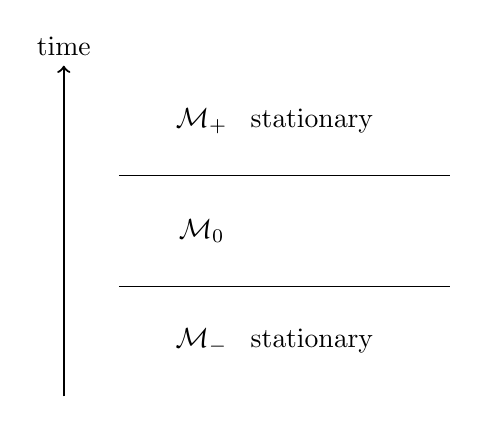
\begin{tikzpicture}[scale=0.7]
        \draw[thick,->] (0,0) -- (0,6) node[above] {time};
        \draw (1,2) -- (7,2);
        \draw (1,4) -- (7,4);
        \node at (2.5,1) {\(\mathcal{M}_-\)};
        \node at (2.5,3) {\(\mathcal{M}_0\)};
        \node at (2.5,5) {\(\mathcal{M}_+\)};
        \node at (4.5,1) {stationary};
        \node at (4.5,5) {stationary};
    \end{tikzpicture}
\end{wrapfigure}
Since \((\mathcal{M}_\pm,g)\) are stationary, there exist for each of them preferred choices of \(S_p^\pm\). Since the spacetime is globally hyperbolic, we can extend these to two choices for the entire spacetime. 

Let \(u_i^\pm\) be orthonormal bases for \(S_p^\pm\), and write \(a_i^\pm=a(u_i^\pm)\). As before, we can write
\begin{equation}
    u_i^\dagger = \sum_j \left(A_{ij}u_j^- + B_{ij}\overline{u_j^-}\right)
\end{equation}
and 
\begin{equation}
    a_i^\dagger = \sum_j \left(\overline{A_{ij}}a_j^- - \overline{B_{ij}}{a_j^-}^\dagger\right).
\end{equation}

Assume there are no particles in \(\mathcal{M}_-\). More concretely, we define the vacua with respect to \(S_p^\pm\) by \(a_i^\pm\ket{0\pm}=0 \Forall i\). Also assume that no particles are present at early times, so that the state is \(\ket{0-}\). The number operator for the \(i^\text{th}\) late time mode is \(N_i^+ = {a_i^+}^\dagger a_i^+\), and its expectation value is
\begin{align}
    \mel{0-}{N_i^+}{0-} &= \mel{0-}{{a_i^+}^\dagger a_i^+}{0-} \\
                        &= \sum_{jk} \mel{0-}{a_k^-(-B_{jk})(-\overline{B_{ij}}){a_j^-}^\dagger}{0-} \\
                        &= \sum_{jk}B_{ij}\overline{B_{ij}} \underbrace{\mel{0-}{a_k^-{a_j^-}^\dagger}{0-}}_{=\delta_{jk}} \\
                        &= \sum_j B_{ij}\overline{B_{ij}} = (BB^\dagger)_{ii}.
\end{align}
Therefore the total expected number of particles is \(\tr(BB^\dagger) = \tr(B^\dagger B)\) (and this is zero iff \(B=0\) i.e.\ iff \(S^+_p=S^-_p\)).

\subsection{Rindler spacetime}
Consider spacetime geometry near the horizon fo a Schwarzschild black hole. We define a new coordinate \(x\) by
\begin{equation}
    r = 2M + \frac{x^2}{8M}
\end{equation}
and expand near \(x=0\). The metric becomes
\begin{equation}
    \dd{s}^2 = -\kappa^2x^2\dd{t}^2 + \dd{x}^2 + (2M)^2 \dd{\Omega}^2 + \dots
\end{equation}
where \(\kappa=\frac{1}{4M}\) is the surface gravity. Ignoring the subleading terms and fixing the spherical coordinates, we obtain \emph{Rindler spacetime} (\(x>0\)):
\begin{equation}
    \dd{s}^2 = -\kappa^2x^2\dd{t}^2 + \dd{x}^2
\end{equation}

Let \(U=-xe^{-\kappa t}>0\) and \(V=xe^{\kappa t}>0\). Then we can write the metric as
\begin{equation}
    \dd{s}^2 = -\dd{U}\dd{V} = -\dd{T}^2 + \dd{X}^2
\end{equation}
where \(U = T-X\) and \(V = T+X\). With these coordinates we can draw a Kruskal diagram:

\begin{figure}[H]
    \centering
    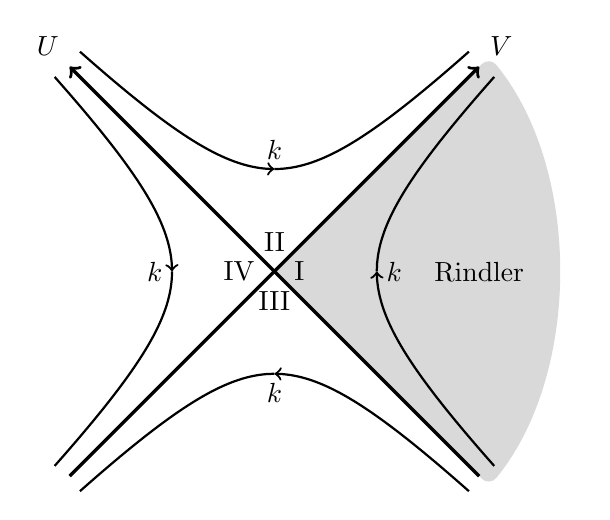
\begin{tikzpicture}[scale=1.3]
        \fill[gray!30, rounded corners] (0,0) -- (2.1,2.1) .. controls (3,1) and (3,-1) .. (2.1,-2.1) -- (0,0);
        \node at (2,0) {Rindler};

        \foreach \k in {0,1,2,3}
        {
            \begin{scope}[rotate={90*\k}]
                \draw[domain={pow(-1,\k)*-1.9}:0,smooth,variable=\x,thick] plot({-sqrt(1+\x*\x))},{\x});
                \draw[domain=0:{pow(-1,\k)*1.9},smooth,variable=\x,<-,thick] plot({-sqrt(1+\x*\x))},{\x});
            \end{scope}
        }
        \node[left] at (-1,0) {\(k\)};
        \node[above] at (0,1) {\(k\)};
        \node[right] at (1,0) {\(k\)};
        \node[below] at (0,-1) {\(k\)};

        \draw (0.1,0) node[right] {I};
        \draw (0,0.1) node[above] {II};
        \draw (0,-0.1) node[below] {III};
        \draw (-0.1,0) node[left] {IV};

        \draw[very thick,->] (-2,-2) -- (2,2) node[above right] {\(V\)};
        \draw[very thick,->] (2,-2) -- (-2,2) node[above left] {\(U\)};
    \end{tikzpicture}
\end{figure}
\(\{U=0\}\cup\{V=0\}\) is a bifurcate Killing horizon of \(k=\pdv{t}\), with surface gravity \(\pm\kappa\). 

We have \(k=\kappa\left(V\pdv{V}-U\pdv{U}\right)\). Consider a ``Rindler observer'' on an orbit of \(k\) (lines of constant \(x\)). The proper acceleration of the observer is given by
\begin{equation}
    A_a = \frac{1}{x}(\dd{x})_a \implies |A| = \frac{1}{x}.
\end{equation}
We use \(k\) to define positive frequency (this differs from the usual Minkowskian definition that uses \(\pdv{T}\)).

\lecture{07/03/16}
Consider a massless scalar field. The Klein-Gordon equation reads
\begin{equation}
    \left(-\pdv[2]{T} + \pdv[2]{X}\right)\phi = \left(-\kappa^2x^2\pdv[2]{t} + \pdv[2]{x}\right)\phi = 0.
\end{equation}
A basis of positive frequency Minkowski modes is given by
\begin{equation}
    u_p(T,X) = c_pe^{-i(\omega T - px)} \qq{where} \sigma = |p|.
\end{equation}
Alternatively, a positive frequency Rindler eigenmode satisfies
\begin{equation}
    \mathcal{L}_k\phi = -i\sigma\phi
\end{equation}
for some \(\sigma>0\). From this, we deduce \(\phi \propto e^{-i\sigma t}\), and solving the K-G equation gives \(\phi \propto e^{-i\sigma t} x^{iP}\), where \(P = \pm \frac{\sigma}{\kappa}\). Hence a basis of positive frequency Rindler modes is given by
\begin{equation}
    u_p^R(T,X) = c_pe^{-i(\sigma t - p \log x)} \qq{where} \sigma = \kappa |p|.
\end{equation}

Let \(N_p\) be the number operator for a Rindler observer, and \(\ket{0}\) the Minkowski vacuum. It can be shown that
\begin{equation}
    \mel{0}{N_p}{0} = \frac{1}{e^{\frac{2\pi\sigma}{\kappa}}-1}.
\end{equation}
A Rindler observer has 4-velocity \(\frac{1}{\kappa x}\pdv{t}=\frac{A}{\kappa}\pdv{t}\), so it measures frequency \(\hat{\sigma} = \frac{A}{\kappa}\sigma\), and we notice that the number of particles follows a Planck spectrum at the Unruh temperature
\begin{equation}
    T_U = \frac{A}{2\pi}.
\end{equation}

\subsection{Wave equation in Schwarzschild solution}
Decompose the field in terms of spherical harmonics:
\begin{equation}
    \phi  = \sum^\infty_{l=0}\sum^{l}_{m=-l}\frac{1}{r}\varphi_{lm}(t,r)Y_{lm}(\theta,\phi)
\end{equation}
The (massless) K-G equation \(\nabla^a\nabla_a\phi=0\) implies
\begin{equation}
    \left[\pdv[2]{t}-\pdv[2]{r_*}+V_l(r_*)\right]\varphi_{lm}=0
\end{equation}
where
\begin{equation}
    V_l(r_*) = \left(1-\frac{2M}{r}\right)\left(\frac{l(l+1)}{r^2} + \frac{2M}{r^3}\right).
\end{equation}

\begin{figure}[H]
    \centering
    \begin{tikzpicture}
        \draw[domain=-3:3,smooth,variable=\x] plot({\x},{2*exp(-(\x-0.4)*(\x-0.4))+0.1});
        \draw[thick,->] (0,-0.5) -- (0,2.5) node[right] {\(V_l\)};
        \draw[thick,->] (-3,0) -- (3,0) node[right] {\(r_*\)};

        \draw[thick,->] (2.6,1.3) -- (3.1,1.3) node[right] {\(\scri^+\)};
        \draw[thick,->] (-2.6,1.3) -- (-3.1,1.3) node[left] {\(\mathcal{H}^+\)};
    \end{tikzpicture}
\end{figure}

Consider a field with arbitrary initial data at \(t=t_0\). For late and early times (large \(|t|\)), the potential vanishes, so the field will decompose into outgoing and ingoing parts:
\begin{equation}
    \varphi_{lm} \approx f_\pm(u) + g_\pm(v) \qq{for} t\to \pm\infty
\end{equation}
\(f_\pm\) and \(g_\pm\) are localised wavepackets, i.e. they vanish for \(|u|\to\infty\) and \(|v|\to\infty\) respectively. Thus we have \(\left.\varphi_{lm}\right|_{\scri^+} = f_+(u)\) and \(\left.\varphi_{lm}\right|_{\mathcal{H}^+}=g_+(v)\), and \(\varphi_{lm}\) is uniquely determined by its behaviour on \(\scri^+\cup\mathcal{H}^+\). 

We define \emph{out} and \emph{down} modes as solutions vanishing on \(\mathcal{H}^+\) and \(\scri^+\) respectively. We can write any solution \(\varphi_{lm}\) as an out modes \(+\) down modes, and the inner product between the two vanishes.

Similarly, define \emph{in} and \emph{up} modes as solutions vanishing on \(\mathcal{H}^-\) and \(\scri^-\) respectively. Any solution can be written as in modes \(+\) down modes, and again their inner products vanish.

\begin{figure}[H]
    \centering
    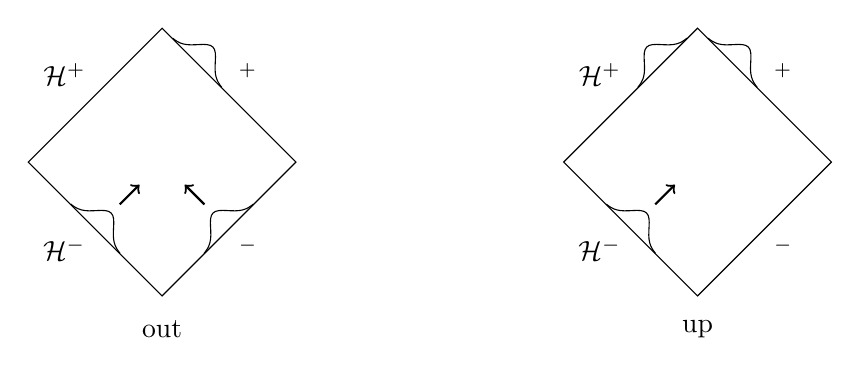
\begin{tikzpicture}[scale=1.7]
        \begin{scope}[shift={(0,0)}]
            \draw (0,0) -- (1,-1) -- (2,0) -- (1,1) -- cycle;
            \node[above left] at (0.5,0.5) {\(\mathcal{H}^+\)};
            \node[below left] at (0.5,-0.5) {\(\mathcal{H}^-\)};
            \node[below right] at (1.5,-0.5) {\(\scri^-\)};
            \node[above right] at (1.5,0.5) {\(\scri^+\)};
            \node at (1,-1.25) {out};

            \begin{scope}[shift={(0.5,-0.5)},scale=0.13,rotate=-45]
                \draw[domain=-2:2,smooth,variable=\x] plot({\x},{1.3*exp(-\x*\x)});
                \draw[thick,->] (0,2) -- (0,3.6);
            \end{scope}
            \begin{scope}[shift={(1.5,-0.5)},scale=0.13,rotate=45]
                \draw[domain=-2:2,smooth,variable=\x] plot({\x},{1.3*exp(-\x*\x)});
                \draw[thick,->] (0,2) -- (0,3.6);
            \end{scope}
            \begin{scope}[shift={(1.26,0.74)},scale=0.13,rotate=-45]
                \draw[domain=-2:2,smooth,variable=\x] plot({\x},{1.3*exp(-\x*\x)});
            \end{scope}
        \end{scope}

        \begin{scope}[shift={(4,0)}]
            \draw (0,0) -- (1,-1) -- (2,0) -- (1,1) -- cycle;
            \node[above left] at (0.5,0.5) {\(\mathcal{H}^+\)};
            \node[below left] at (0.5,-0.5) {\(\mathcal{H}^-\)};
            \node[below right] at (1.5,-0.5) {\(\scri^-\)};
            \node[above right] at (1.5,0.5) {\(\scri^+\)};
            \node at (1,-1.25) {up};

            \begin{scope}[shift={(0.5,-0.5)},scale=0.13,rotate=-45]
                \draw[domain=-2:2,smooth,variable=\x] plot({\x},{1.3*exp(-\x*\x)});
                \draw[thick,->] (0,2) -- (0,3.6);
            \end{scope}
            \begin{scope}[shift={(1.26,0.74)},scale=0.13,rotate=-45]
                \draw[domain=-2:2,smooth,variable=\x] plot({\x},{1.3*exp(-\x*\x)});
            \end{scope}
            \begin{scope}[shift={(0.74,0.74)},scale=0.13,rotate=45]
                \draw[domain=-2:2,smooth,variable=\x] plot({\x},{1.3*exp(-\x*\x)});
            \end{scope}
        \end{scope}
    \end{tikzpicture}
\end{figure}
Consider \(\phi\propto e^{-i\omega t}\), \(\phi_{\omega l m} = \frac{1}{r} e^{-i\omega t}R_{\omega l m}(r)Y_{lm}(\theta,\phi)\), \(\omega>0\). We say that \(\phi\) is ``positive frequency'' if we can write it as a superposition of \(\phi_{\omega l m}\). If we substitute \(\varphi_{lm} = e^{-i\omega t}R_{\omega l m}\) into the wave equation, we obtain
\begin{equation}
    \left[-\pdv[2]{r_*} + V_l(r_*)\right] R_{\omega l m} = \omega^2 R_{\omega l m}.
\end{equation}
Since the potential vanishes for \(|r_*| \to \infty\), we have asymptotically \(R_{\omega l m} \sim e^{\pm i \omega r_*}\). Therefore
\begin{equation}
    \phi_{\omega l m} \propto e^{-i\omega(t\mp r_*)} = 
    \begin{cases}
        e^{-i\omega u} & \text{outgoing}\\
        e^{-i\omega v} & \text{ingoing}
    \end{cases}.
\end{equation}

\subsection{Hawking radiation}
Consider a collapsing star. This is time dependent, so we expect some particle production. Surprisingly, this particle production persists to late times.

Since \(\mathcal{H}^- = \varnothing\), there are no up modes. Let \(\{f_i\}\) be a basis for in modes with positive frequency near \(\scri^-\), \(\{p_i\}\) be a basis for out modes with positive frequency near \(\scri^+\), and \(\{q_i,\overline{q_i}\}\) be a basis of down modes. Thus we have two different bases for \(S\): \(\{f_i,\overline{f_i}\}\) and \(\{p_i,\overline{p_i},q_i,\overline{q_i}\}\). We assume that both bases are orthonormal.

\begin{wrapfigure}{l}{0.5\linewidth}
    \centering
    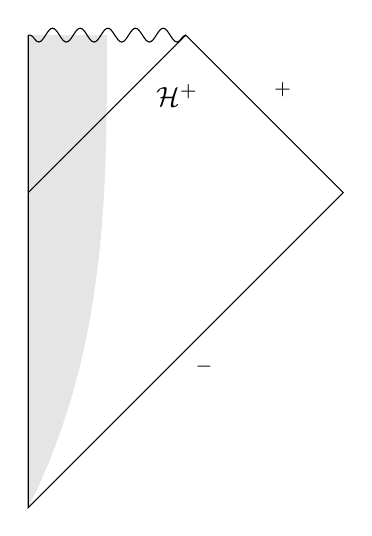
\begin{tikzpicture}[]
        \fill[gray!20] (0,6) -- (0,0) .. controls (1,2) and (1,4) .. (1,6) -- cycle;
        \draw (0,6) -- (0,0) -- (4,4) -- (2,6) -- (0,4);
        \draw[decorate,decoration=snake] (2,6) -- (0,6);
        
        \node[above right] at (3,5) {\(\scri^+\)};
        \node[below right] at (2,2) {\(\scri^-\)};
        \node[below right] at (1.5,5.5) {\(\mathcal{H}^+\)};
    \end{tikzpicture}
\end{wrapfigure}
Let \(a_i = (f_i,\phi)\) and \(b_i = (p_i,\phi)\) be annihilators for the in and out modes respectively. We can expand
\begin{equation}
    p_i = \sum_j\left(A_{ij}f_j + B_{ij}\overline{f_j}\right),
\end{equation}
and as before we obtain
\begin{equation}
    b_i = \sum_j\left(\overline{A_{ij}}a_j - B{ij}a_j^\dagger\right).
\end{equation}
Assume that the state is the ``in'' vacuum \(\ket{0}\), i.e.\ \(a_i \ket{0}=0\) for all \(i\). The expected number of particles in the \(i^\text{th}\) out mode is
\begin{equation}
    \mel{0}{b_i^\dagger b_i}{0} = (BB^\dagger)_{ii}.
\end{equation}

\lecture{09/03/16}
In order to calculate this, we will need to determine the Bologiubov coefficients \(B_{ij}\).

\begin{wrapfigure}{r}{0.4\linewidth}
    \centering
    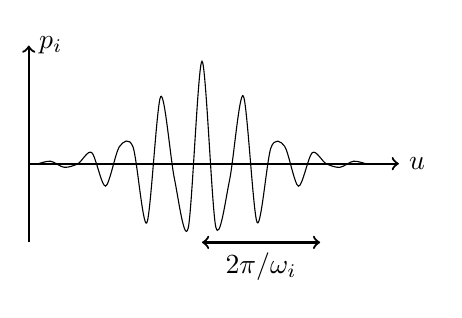
\begin{tikzpicture}
        \draw[domain=-2.1:2.1,smooth,step=0.05cm,variable=\x] plot({\x},{1.3*cos(2800*\x)*exp(-\x*\x)});
        \draw[thick,->] (-2.2,0) -- (2.5,0) node[right] {\(u\)};
        \draw[thick,->] (-2.2,-1) -- (-2.2,1.5) node[right] {\(p_i\)};
        \draw[thick,<->] (0,-1) -- (1.5,-1) node[midway,below] {\(2\pi/\omega_i\)};
    \end{tikzpicture}
\end{wrapfigure}
We choose the \(p_i\) such that \(\left.p_i\right|_{\scri^+}\) are wavepackets with frequencies near \(\omega_i > 0\), and \(f_i\) such that \(\left.f_i\right|_{\scri^-}\) are wavepackets with the save \(v\)-dependence as the \(u\)-dependence of \(\left.p_i\right|_{\scri^+}\).

For the moment, just consider Kruskal spacetime, and imagine propagating the wavepacket \(p_i\) backwards in time. Part of the wavepacket would be reflected to \(\scri^-\), and part would be transmitted to \(\mathcal{H}^-\). Thus we can write \(p_i = p_i^{(1)} + p_i^{(2)}\), where \(p_i^{(1)}\) is an in mode and \(p_i^{(2)}\) is an up mode.

\begin{figure}[H]
    \centering
    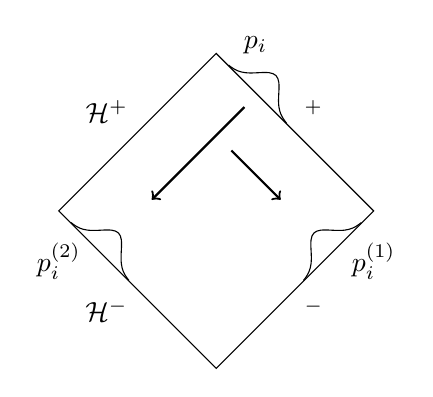
\begin{tikzpicture}[scale=2]
        \draw (0,0) -- (1,-1) -- (2,0) -- (1,1) -- cycle;
        \node[above left] at (0.5,0.5) {\(\mathcal{H}^+\)};
        \node[below left] at (0.5,-0.5) {\(\mathcal{H}^-\)};
        \node[below right] at (1.5,-0.5) {\(\scri^-\)};
        \node[above right] at (1.5,0.5) {\(\scri^+\)};

        \begin{scope}[shift={(0.26,-0.26)},scale=0.13,rotate=-45]
            \draw[domain=-2:2,smooth,variable=\x] plot({\x},{1.3*exp(-\x*\x)});
            \draw[thick,->] (0,10) -- (0,3.6);
        \end{scope}
        \begin{scope}[shift={(1.74,-0.26)},scale=0.13,rotate=45]
            \draw[domain=-2:2,smooth,variable=\x] plot({\x},{1.3*exp(-\x*\x)});
            \draw[thick,->] (0,7) -- (0,3.6);
        \end{scope}
        \begin{scope}[shift={(1.26,0.74)},scale=0.13,rotate=-45]
            \draw[domain=-2:2,smooth,variable=\x] plot({\x},{1.3*exp(-\x*\x)});
        \end{scope}

        \node at (1.25,1.05) {\(p_i\)};
        \node at (0,-0.32) {\(p_i^{(2)}\)};
        \node at (2,-0.32) {\(p_i^{(1)}\)};
    \end{tikzpicture}
\end{figure}

The \emph{reflection coefficient} is \(R_i=\sqrt{(p_i^{(1)},p_i^{(1)})}\), and the \emph{transmission coefficient} is \(T_i=\sqrt{(p_i^{(2)},p_i^{(2)})}\). Since \((p_i,p_i)=1\), we have \(R_i^2+T_i^2=1\) (since the in and up modes are orthogonal). Time reversal symmetry implies that \(R_i\) is the fraction of \(f_i\) reflected to \(\scri^+\), and \(T_i\) is the fraction of \(f^i\) crossing \(\mathcal{H}^+\).

\begin{figure}[H]
    \centering
    \begin{tikzpicture}[]
        \fill[gray!20] (0,6) -- (0,0) .. controls (1,2) and (1,4) .. (1,6) -- cycle;
        \draw (0,6) -- (0,0) -- (4,4) -- (2,6) -- (0,4);
        \draw[decorate,decoration=snake] (2,6) -- (0,6);
        
        \begin{scope}[shift={(2.5,5.5)},scale=0.25,rotate=-45]
            \draw[domain=-2:2,smooth,variable=\x] plot({\x},{1.3*exp(-\x*\x)});
        \end{scope}
        \begin{scope}[shift={(3.5,3.5)},scale=0.25,rotate=45]
            \draw[domain=-2:2,smooth,variable=\x] plot({\x},{1.3*exp(-\x*\x)});
        \end{scope}
        \begin{scope}[shift={(1.5,1.5)},scale=0.25,rotate=45]
            \draw[domain=-2:2,smooth,variable=\x] plot({\x},{1.3*exp(-\x*\x)});
        \end{scope}
        \draw[dashed] (2.5,5.5) -- (0,3) -- (1.5,1.5);
        \draw[dashed] (3.5,3.5) -- (2,5);
        \node[below right] at (3.5,3.5) {\(p_i^{(1)}\)};
        \node[below right] at (1.5,1.5) {\(p_i^{(2)}\)};
        \node[above right] at (2.8,5.8) {\(p_i\)};
    \end{tikzpicture}
\end{figure}
Now return to the collapsing matter spacetime.
We are interested in \(p_i\) localised at late retarded time. Because of this \(p_i^{(1)}\) is localised at late advanced time \disapprove, so scattering happens outside ths collapsing matter, and \(p_i^{(1)}\) is the same as for the Kruskal spacetime. \(p_i^{(1)}\) does not experience the non-stationary geometry and so is positive frequency on \(\scri^-\). As above, \((p_i^{(1)},p_i^{(2)}) = R_i^2\). Thus in the Bogoliubov transformation
\begin{equation}
    p_i^{(1,2)} = \sum_j\left(A_{ij}^{(1,2)}f_j + B_{ij}^{(1,2)}\overline{f_j}\right),
\end{equation}
we have \(B_{ij}^(1)=0\). Let \(A_{ij} = A_{ij}^{(1)} + A_{ij}^{(2)}\) and \(B_{ij} = B_{ij}^{(2)}\). Since \((p_i^{(1)},p_i^{(2)}) = 0\) and \((p_i,p_i)=1\), we have \((p_i^{(2)},p_i{(2)})=1-R_i^2=T_i^2\).

Note that \(\mathcal{H}^+\) is at \(u=\infty\), so for a wavepacket on \(\scri^+\) at late retarded times there are infinitely many oscillations close to \(\mathcal{H}^+\), and hence an observer crossing the horizon measures a very large frequency.
\begin{figure}[H]
    \centering
    \begin{tikzpicture}[scale=1.5]
        \fill[gray!20] (0,6) -- (0,0) .. controls (1,2) and (1,4) .. (1,6) -- cycle;
        \draw (0,6) -- (0,0) -- (4,4) -- (2,6) -- (0,4);
        \draw[decorate,decoration=snake] (2,6) -- (0,6);
        
        \begin{scope}[shift={(2.5,5.5)},scale=0.25,rotate=-45]
            \draw[domain=-2:2,smooth,variable=\x] plot({\x},{1.3*exp(-\x*\x)});
        \end{scope}
        \begin{scope}[shift={(1.5,1.5)},scale=0.25,rotate=45]
            \draw[domain=-2:2,smooth,variable=\x] plot({\x},{1.3*exp(-\x*\x)});
        \end{scope}
        \foreach \i in {1,2,3,4,5,6,7,8,9}
        {
            \draw ({1.75+0.75/sqrt(\i)},{6.25-0.75/sqrt(\i)}) -- (0,{4.5-1.5/sqrt(\i)}) -- ({2.25-0.75/sqrt(\i)},{2.25-0.75/sqrt(\i});
        }
        \draw (0,4) -- (2,2);
        \fill (2,2) circle (0.06) node[below right] {\(v=0\)};
        \fill (1.5,1.5) circle (0.06) node[below right] {\(v_0<0\)}; 
    \end{tikzpicture} 
\end{figure}

As there is a large frequency, we can use the approximation of geometric optics, and set 
\begin{equation}
    \phi(x)=A(x) = e^{i\lambda S(x)},
\end{equation}
where \(\lambda\gg1\) and \(S(x)\) is the phase. \(\nabla^2\phi=0\) implies \((\nabla S)^2=0\), so \(S=\text{constant}\) are null hypersurfaces.

Consider then the null geodesic congruence containing the generators of \(\mathcal{H}^+\) and surfaces of constant \(S\). As previously, let \(U\) be the tangent vector field to the geodesics in the congruence, and let \(N\) be a null vector field such that \(N\vdot U=-1\) and \(U\vdot\nabla N^a=0\). Write \(S^a = \alpha U^a + \hat{S}^a + \beta N^a\) where \(\alpha U^a + \hat{S}^a\) is the part orthogonal to \(U^a\) and tangent to \(\mathcal{H}^+\), and \(beta N^a\) points off of \(\mathcal{H}^+\) towards generators of surfaces \(S=\text{constant}\).

\begin{wrapfigure}{l}{0.5\linewidth}
    \centering
    \begin{tikzpicture}[scale=1.3]
        \draw (0,0) -- (3,3) node[above] {\(\mathcal{H}^+\)};
        \draw[->,thick] (0.68,0.68) -- (0.7,0.7) node[left] {\(\gamma\)};
        \draw (0.7,-0.7) -- (3.7,2.3);
        \draw[->,thick] (1.38,-0.02) -- (1.4,0) node[below] {\(\gamma'\)};

        \draw[->,very thick] (1.5,1.5) -- (0.5,2.5) node[above left] {\(N^a\)};
        \draw[->,very thick] (1.5,1.5) -- (2.5,2.5) node[above left] {\(U^a\)};
        \draw[->,very thick] (1.5,1.5) -- (2.2,0.8) node[above right, midway] {\(-\epsilon N^a\)};
    \end{tikzpicture}
\end{wrapfigure}
Let \(\gamma\) be a generator of \(\mathcal{H}^+\), and \(\gamma'\) a generator of a constant \(S\) surface close to \(\mathcal{H}^+\). By spherical symmetry, we can choose \(N^\theta = N^\phi=0\). Outside the matter, \(\pdv{V}\) is tangent to the affinely parametrised generators of \(\mathcal{H}^+\), so we can choose \(U^a=\left(\pdv{V}\right)^a\). \(N^2=0,U\vdot N=-1\) then give \(N=C\pdv{U}\), where \(C>0\) is a constant given by \(g_{UV}\).

\(\gamma\) has \(U=0\), so \(\gamma'\) has \(U=-\epsilon C\) for some small \(\epsilon\) (since we are considering late time modes and are outside matter). We have \(u = - \frac{1}{\kappa}\log(-U)\), and therefore \(\gamma'\) is a null geodesic with
\begin{equation}
    u = - \frac{1}{\kappa}\log(\epsilon C).
\end{equation}

Let \(F(u)\) denote the phase of the wavepacket \(p_i\) on \(\scri^+\). Then the phase \emph{everywhere} on \(\gamma'\) is 
\begin{equation}
    S=F\left(-\frac{1}{\kappa}\log(\epsilon C)\right).
\end{equation}

Near \(\scri^-\), \(\gamma\) and \(\gamma'\) are ingoing radial null geodesics, so \(U^a\propto\left(\pdv{u}\right)^a\) in \((u,v)\) coordinates. Near \(\scri^-\), the metric is
\begin{equation}
    \dd{s}^2\approx -\dd{u}\dd{v} + \frac{1}{4} (u-v)\dd{\Omega}^2.
\end{equation}
Spherical symmetry, \(N^2=0\), \(U\vdot N=-1\) together imply that \(\left.N\right|_{\scri^-}=D^{-1}\pdv{v}\), where \(D>0\) is a constant. From this we have that \(\gamma'\) intersects \(\scri^-\) at \(v=\epsilon D^{-1}\), and thus on \(\scri^-\) at small \(v\) the phase is
\begin{equation}
    S = F\left(-\frac{1}{\kappa}\log(CDv)\right).
\end{equation}
Hence we have
\begin{equation}
    \left.p_i^{(2)}\right|_{\scri^-} \approx
    \begin{cases}
        0 & v > 0 \\
        A(v)\exp\left[iF\left(-\frac{1}{\kappa}\log(CDv)\right)\right] & \text{small \(v<0\)},
    \end{cases}
\end{equation}
where the amplitude \(A(v)\) is some smooth function of \(v\).

\lecture{11/03/16}
At the expense of some rigour, we will now drop the wavepacket treatment and assume that we are dealing with plane waves, so that \(F(u)=-i\omega_i u\). We will write \(p_\omega\) instead of \(p_i\), so that
\begin{equation}
    \left.p_\omega^{(2)}\right|_{\scri^-} \approx
    \begin{cases}
        0 & v > 0 \\
        A_\omega(v)\exp\left[\frac{i\omega}{\kappa}\log(CDv)\right] & \text{small \(v<0\)}.
    \end{cases}
\end{equation}
Similarly, use a basis of in modes labelled by their frequencies
\begin{equation}
    \left.f_\sigma\right|_{\scri^-} = (2\pi N_\sigma)^{-1} e^{-i\sigma v},\quad \sigma > 0.
\end{equation}
Writing \(p_\omega^{(2)}\) in terms of the \(f_\sigma\) is just the same as finding its Fourier transform. We have
\begin{equation}
    \tilde{p}_\omega^{(2)}(\sigma) = A_\omega\int_{-\infty}^0 \dd{v} e^{i\sigma v} \exp\left[\frac{i\omega}{\kappa}\log(-CDv)\right].
\end{equation}
where we have approximated \(A_\omega\) is constant since \(p_\omega^{(2)}\) is non-zero for a small portion of \(v\). The inverse is
\begin{align}
    p_\omega^{(2)}(v) &= \int^\infty_{-\infty} \frac{\dd{\sigma}}{2\pi} e^{-i\sigma v} \tilde{p}_\omega^{(2)}(\sigma) \\
                      &= 
    \underbrace{\int_0^\infty \dd{\sigma} N_\sigma \tilde{p}_\omega^{(2)}(\sigma)f_\sigma(v)}_{\text{positive frequency}}
    +
    \underbrace{\int_0^\infty \dd{\sigma} \overline{N_\sigma} \tilde{p}_\omega^{(2)}(-\sigma)\overline{f_\sigma(v)}}_{\text{negative frequency}}.
\end{align}
Hence we can write down some Bogoliubov coefficients:
\begin{equation}
    A^{(2)}_{\omega\sigma} = N_\sigma\tilde{p}_\omega^{(2)}(\sigma),\quad
    B_{\omega\sigma} = \overline{N_\sigma}\tilde{p}_\omega^{(2)}(-\sigma)\quad
    (\omega,\sigma > 0)
\end{equation}
In order to evaluate the Fourier transform we will complete the contour of integration in the complex plane. We choose the branch of \(\log\) to be the one given by \(\log|z| + i\arg z\), where \(\arg z \in \left(-\frac{\pi}{2},\frac{3\pi}{2}\right)\).

Consider \(\tilde{p}_\omega^{(2)}(-\sigma)\) for \(\sigma > 0\). We close the contour in the \(v\)-plane in the following way:
\begin{figure}[H]
    \centering
    \begin{tikzpicture}
        \fill (0,0) circle (0.06);
        \draw[decorate,decoration=snake] (0,0) -- (0,2.5);
        \draw (0.15,0) -- (2.5,0) arc (0:-180:2.5) -- (-0.15,0) arc (-180:0:0.15);

        \draw[thick,->] (1.24,0) -- (1.25,0);
        \draw[thick,->] (-1.26,0) -- (-1.25,0);
        \draw[thick,->] (0.01,-2.5) -- (-0.01,-2.5);

        \draw[thick,<->,rotate=-20] (0,-0.2) -- (0,-2.45) node[midway,right] {\(R\to\infty\)}; 
    \end{tikzpicture}
\end{figure}
By Jordan's lemma, the contribution of the large semi-circular part of the contour vanishes. Hence
\begin{align}
    \tilde{p}_\omega^{(2)}(-\sigma) &= -A_\omega\int_0^\infty \dd{v} e^{-i\sigma v}\exp\left[\frac{i\omega}{\kappa}\log(-CDv)\right] \\
                                    &= -A_\omega\int_0^\infty \dd{v} e^{-i\sigma v}\exp\left[\frac{i\omega}{\kappa}\left(\log(CDv)+i\pi\right)\right] \\
                                    &= -A_\omega e^{-\frac{\pi\omega}{\kappa}} \int^0_{-\infty} \dd{v} e^{i\sigma v} \exp\left[\frac{i\omega}{\kappa}\log(-CDv)\right] \quad (v\to-v) \\
                                    &= -e^{-\frac{\pi\omega}{\kappa}} \tilde{p}_\omega^{(2)}(\sigma).
\end{align}
Therefore \(|B_{\omega\sigma}| = e^{-\frac{\pi\omega}{\kappa}} |A^{(2)}_{\omega\sigma}|\). Returning to wavepackets, the corresponding result is
\begin{equation}
    |B_{ij}| = e^{-\frac{\pi\omega_i}{\kappa}} |A^{(2)}_{ij}|.
\end{equation}
Note that 
\begin{equation}
    T_i^2 = (p_i^{(2)},p_i^{(2)}) = \sum_j\left(|A^{(2)}_{ij}|^2 - |B_{ij}|^2\right) = \left(e^{\frac{2\pi\omega_i}{\kappa}}-1\right)\sum_j|B_{ij}|^2,
\end{equation}
and \(\sum_j|B_{ij}|^2=(BB^\dagger)_{ii}=\mel{0}{b_i^\dagger b_i}{0}\), so we have
\begin{equation}
    \mel{0}{b_i^\dagger b_i}{0} = \frac{\Gamma_i}{e^{\frac{2\pi\omega_i}{\kappa}}-1},
\end{equation}
where \(\Gamma_i=T_i^2\) is the \emph{absorption cross-section} for the mode \(f_i\). This is exactly a blackbody spectrum at the black hole's \emph{Hawking temperature}
\begin{equation}
    T_H = \frac{\kappa}{2\pi}.
\end{equation}
Note that \(T_H\approx 6\times10^{-8}\times\frac{M_{\astrosun}}{M}\,\text{K}\), and the CMB is at a temperature of \(2.7\,\text{K}\), so the effect of this \emph{Hawking radiation} is cosmologically negligible.

\subsection{Black hole thermodynamics}
Hawking radiation implies that a black hole is a thermodynamic object at temperature \(T_H\). The zeroth law of BH mechanics is just the application of the zeroth law of thermodynamics to the black hole. Writing the first law as
\begin{equation}
    \dd{E} = T_H \dd{S_{BH}} + \omega_H\dd{J},
\end{equation}
we see that the entropy associated with the black hole is
\begin{equation}
    S_{BH} = \frac{A}{4} = \frac{c^3A}{4G\hbar}.
\end{equation}
Note that \(S_{BH}\) can decrease quantum mechanically. We therefore make a generalisation of the second law to saying that \(S_{BH}+S_{\text{matter}}\) is non-decreasing (this holds in Hawking radiation). 

Note that if most of the energy in the universe was in the form of black holes, the total entropy in the universe would be far higher than it currently is -- the universe seems to be in a special low entropy state.

Statistical mechanics gives that the number of quantum microstates of the black hole as \(N\sim \exp^{S_{BH}}\). A replication of this result is a major goal of quantum gravity research.

\subsection{Black hole evaporation}
The energy of Hawking radiation must come from the black hole itself. Stefan's law for energy loss from a blackbody gives
\begin{equation}
    \dv{E}{t} \approx - \alpha A T^4
\end{equation}
where \(\alpha\) is a dimensionless constant, and we approximate \(\gamma_i\) by treating the black hole as a perfectly absorbing sphere of area \(A\). Plugging in \(E=M\), \(A\propto M^2\) and \(T=T_H\propto\frac{1}{M}\) gives
\begin{equation}
    \dv{M}{t}\propto -\frac{1}{M^2}.
\end{equation}
Hence we have \(M\to0\) in a finite time \(\tau \sim M^3 \sim 10^{71}(\frac{M}{M_{\astrosun}})^3\,\text{seconds}\).

Black hole evaporation gives rise to the so-called \emph{information paradox}. Consider the following sequence of events. A star is initially in a pure quantum state. It collapses to a black hole, and then evaporates. The final state is completely composed of thermal radiation which must be a mixed state. So we have gone from a pure state to a mixed state, but this is impossible in quantum mechanics!

Information about the initial state is lost, and the only information that remains is the energy, angular momentum and charge of the black hole.

\end{document}

